%Thesis Main Page used with thesis.sty (Dorothea Brosius, September 2007) based on the
%University of Maryland Electronic Thesis and Dissertation (ETD) Style Guide

%Adapted for use at the University of Colorado, Colorado Springs by Suzette Stoutenberg and Jeremy Witmer

\documentclass[11pt]{thesis}
\usepackage[utf8]{inputenc}
\usepackage{lscape}
\usepackage{indentfirst}
\usepackage{latexsym}
\usepackage[titletoc,toc]{appendix}
\usepackage{multirow}
\usepackage{tabls}
\usepackage{wrapfig}
\usepackage{slashbox}
\usepackage{longtable}
\usepackage{amssymb}
\usepackage{amsmath}
\usepackage{algorithm}
\usepackage{algorithmic}
\usepackage{cite}
\usepackage[hyphens]{url}
%\usepackage{hyperref}
% when uncommenting hyperref, uncomment phantom section below
\usepackage{boxedminipage}
\usepackage{listings}
\usepackage{ifpdf}
\usepackage{verbatim}
\usepackage{color}
\usepackage{pdflscape}
\usepackage{booktabs}
\usepackage{tabularx}
\usepackage{caption}
\usepackage{setspace}
\doublespacing

\ifpdf
	\usepackage[pdftex]{graphicx}
\else
	\usepackage{graphicx}
\fi

\ifpdf
	\DeclareGraphicsExtensions{.pdf, .jpg, .tif, .png}
\else
	\DeclareGraphicsExtensions{.eps, .jpg}
\fi

\renewcommand{\topfraction}{0.85}
\renewcommand{\textfraction}{0.1}
\renewcommand{\floatpagefraction}{0.75}

\renewcommand{\baselinestretch}{2}
\setlength{\textwidth}{6in}
\setlength{\textheight}{9in}
\setlength{\topmargin}{-.50in}
%\setlength{\topmargin}{0in}    %use this setting if the printer makes the the top margin 1/2 inch instead of 1 inch
\setlength{\oddsidemargin}{.5in}

\clubpenalty=10000
\widowpenalty=10000

\begin{document}

\pagenumbering{roman}
%Everything on these pages needs to be lower Roman numeral

% Front Page
\title{\bf {\LARGE Using Evolutionary Computing to Develop Game Strategy for a Non-Deterministic Game}}
\author{by \\ Kevin Mukhar \\  B.A., University of Washington, 1983 \\ 
M.S., University of Northern Colorado, 1993 
\\
\\
\\ A thesis submitted to the Graduate Faculty of the \\
University of Colorado at Colorado Springs \\
in partial fulfillment of the \\
requirements for the degree of \\
Master of Science \\
Department of Computer Science \\
2013 }
\date{}

\maketitle

\setcounter{page}{2}

%Copyright Page
\newpage

\pagestyle{plain}

\begin{minipage}[t]{5.0in}
	\vspace{7.0in}
	\bf \copyright \ Copyright By Kevin Mukhar 2013 \\[-1.0pc]
	Some Rights Reserved (See Appendix L) \rm
\end{minipage}



%Signatures Page
\newpage

\begin{center}
	This thesis for the Master of Science degree by \\
	Kevin Mukhar \\
	has been approved for the \\
 	Department of Computer Science \\
	by \\ 
	\vspace{3.0pc}
	\makebox[3in]{\hrulefill} \\[-1.0pc]
	Jugal Kalita, Chair \\
	\vspace{3.0pc}
	\makebox[3in]{\hrulefill} \\[-1.0pc] 
	Sudhanshu Semwal \\
	\vspace{3.0pc}
	\makebox[3in]{\hrulefill} \\[-1.0pc] 
	Rory Lewis \\
\end{center}


\begin{flushright}
	\vspace{2.0pc}
	\makebox[2in]{\hrulefill} \\[-1.0pc]
	Date
\end{flushright}


%Abstract
\newpage

\setlength{\parindent}{0in}
Mukhar, Kevin (M.S., Computer Science) 

Using Evolutionary Computing to
Develop Game Strategy for a Non-Deterministic Game 

Thesis directed by Professor Jugal Kalita

\vspace{28pt}
\setlength{\parindent}{.4in}

Games and game theory are rich fields of study for artificial intelligence (AI)
and evolutionary computation. It is known that games can be used to teach
knowledge and skills. Games can also be used to model real-world situations. If
humans, or other animals, can learn to play games successfully, it is
reasonable to theorize that a computational based AI can also learn to play
games. A great deal of research has been conducted into using AI to solve
deterministic games with complete information. However, less research has
been conducted into non-deterministic games. This thesis investigates the use of
evolutionary computation techniques to evolve game strategies for the
multi-player non-deterministic game Monopoly.

%Dedication Page
\newpage

\parbox{5.0in}{
	\vspace{2.0in}
	\begin{center}
		{\large{\emph{TBD Dedication goes here \\ can break across two lines}}}
	\end{center}
}


%Acknowledgments
\newpage
\begin{center}
	{\large{\bf Acknowledgments}}
\end{center}
\setlength{\parindent}{.4in}

I wish to thank Dr. Jugal Kalita for his guidance throughout the project.

I also wish to thank the following individuals who played numerous games
of Monopoly against the AI players to test whether the players had evolved to a
human level of competition:

Anne M.

Barbara M.

Kristen J.

Christine M.

Hillary L.

Shirley M.

Beth H.

Marin J.

Evan J.

Greg B.

Luis A.-M.

Tom H. %This is all title pages, acknowledgments, copyright, etc.

\newpage
%\small\normalsize
\tableofcontents %(required, lower-case Roman)

%\newpage
\setlength{\parskip}{1em}
\clearpage
%\phantomsection
%\addcontentsline{toc}{chapter}{List of Tables}
\listoftables %(if present,
% lower-case Roman)

%\newpage
\clearpage
%\phantomsection
%\addcontentsline{toc}{chapter}{List of Figures}
\listoffigures %(if present,
% lower-case Roman)

\newpage
\setlength{\parskip}{0em}
\small\normalsize
\setcounter{tocdepth}{2}

\pagenumbering{arabic}
\setcounter{page}{1}

\setlength{\parindent}{.4in}

\lstset{
  breaklines=true,
  language=XML,
  frame=ltrb,
  framesep=5pt,
  basicstyle=\normalsize
}

\clearpage
\chapter{Introduction}\label{chap:intro}
Games can be used to study many different real world problems. In the
classic monograph by John Von Neumann and Oskar Morgenstern, \emph{Theory of
Games and Economic Behavior}, it was applied to economics and economic behavior
\cite{neumann1944theory}.

Early work by mathematicians studying card and dice games led to the development
of statistics and probability \cite{hald1990history,rudas2008handbook}. Games
can be studied from a sociological point of view, looking at how social behavior
and human interactions affect and are affected by game play
\cite{fararo1992meaning}. As mentioned previously, games can be studied as a
model of economics and decision making \cite{neumann1944theory}. A great deal of
artificial intelligence research deals with developing AI game players and
finding optimum game strategies \cite{russell2010artificial}.

\section{Objective}

Early research into AI and games tended to focus on developing algorithms for
searching the space of legal moves. This research led to such techniques as the
Min-Max algorithm~\cite{neumann1944theory} and the A* search
algorithm~\cite{Hart_Nilsson_Raphael_1968,Hart:1972:LFB:1056777.1056779}. The
Min-Max algorithm was originally developed by Von Neumann as a way to develop
the best move in a 2-person zero-sum game with complete information. Although
originally developed for a 2-person game, the min-max theorem has been extended
to cover any number of players. The A* algorithm is a method to find the least
cost path in traversing a search space or graph.

With the development of genetic algorithms and evolutionary computation,
re\-search\-ers in this area have investigated many games in attempts to show
that optimal strategies for games can be evolved. Much of that research has
focused on two player deterministic games like The Prisoner's
Dilemma~\cite{Flood1958} and Tic-Tac-Toe. Evolutionary computation techniques
have been used with good success for these types of
problems~\cite{DBLP:conf/cig/QuekG07,Fogel1993}.

There are other classes of games, however, such as multi-player
non-deterministic games where the search space is potentially quite large and
the cost function could have multiple local and global
optima~\cite{condon1992complexity,condon1993algorithms,Walker:gamebe:2011}. Any
game that relies on some form of non-determinism (i.e., rolling dice, shuffling
cards, etc.) falls into this category. Evolutionary computation could be an
effective approach to these types of problems because it provides the capability
to traverse a large search space and find optimal
strategies~\cite{Quek_GAPoker,Foster1990219,eriksson2001evolution}.

This paper documents experiments that investigated using evolutionary
computation to evolve game strategies for a non-deterministic game. In general,
the experiments studied whether genetic algorithms can be used to develop
strategies for a non-deterministic games or a game with incomplete knowledge.

\section{Organization of Thesis}

The thesis investigated evolutionary computing as a means to develop game
playing strategies. Since the primary subject matter of this thesis is genetic
algorithms, we start in Chapter \ref{chap:geneticAlgorithms} with a brief
overview of genetic algorithms.

Chapter \ref{chap:background} provides a survey of some previous research into
evolutionary computation and games that will be applied in this thesis. We will
look at both practical and theoretical research that applied evolutionary
computing to various games.

The game known as Monopoly was chosen as the subject of this research. Chapter
\ref{chap:monopoly} provides details about Monopoly, focusing on the rules of
the game.

The details of how a genetic algorithm will be used in this research is provided
in Chapter \ref{chap:algorithm}. We look at various formats for the genome,
along with different options for measuring genome fitness, and the process for
propagating a population.

Using the parameters in \ref{chap:algorithm}, populations of players are created
and then played in simulated Monopoly tournaments. The populations are evolved
and then they compete again with the goal of generating better players. The
results of the evolutionary process are detailed in Chapter \ref{chap:results}.

Chapter \ref{chap:conclusion} concludes the thesis by sumarizing and discussing
the results.

\clearpage
\chapter{Genetic Algorithms}\label{chap:geneticAlgorithms}

Genetic algorithms are used to model optimization problems and to find solutions
to those problems using techniques borrowed from natural
evolution~\cite{Holland1992,goldberg1989genetic,fogel2000evolutionary}. In
nature, populations of individuals exist in some environment. Individuals that
are more fit in their environment are more likely to survive to pass on their
genes to new individuals, leading to the overall population being more fit.

Likewise in genetic algorithms there are populations of solutions. Those
solutions that are more fit in the solution space are more likely to pass their
genes to a new population either through reproduction, recombination, or
mutation. Over time, the population tends to have more fit solutions.

Genetic algorithms can be used to find approximate solutions to problems that
are considered to be intractable.

We begin with a very brief summary of the complexity class
NP~\cite{alsuwaiyel1999algorithms,Cormen:2009:IAT:1614191} and list some
examples of those types of problems. There are various ways to tackle NP
problems such as approximation, the Monte Carlo method, and
heuristics~\cite{russell2010artificial}. None of those methods can guarantee an
exact solution, just a ``good enough'' solution.

Another way to get an approximate solution is to use a genetic algorithm. A
genetic algorithm is similar to the Monte Carlo method, in that a set of
solutions is created randomly. But unlike randomization, we do not continue to
generate more random solutions in the hopes of stumbling on a better solution.
The development of better solutions in a genetic algorithm is guided by
selection pressures which eliminate poor solutions and evolve good solutions
into better solutions.

After looking at the basic genetic algorithm, we briefly discuss various ways to
modify the standard genetic algorithm to expand its ability to find solutions to
problems. These enhancements allow genetic algorithms to be applied to a large
set of problems.

\section{NP Problems}

In complexity theory, there are a number of classes that are used to categorize
problems~\cite{alsuwaiyel1999algorithms,Cormen:2009:IAT:1614191}. The simplest
of those classes is the class P: those problems which can be deterministically
solved in polynomial time. Using big O notation, we write
\begin{equation*}
P \in O(n^{k})
\end{equation*}
where \(n\) is the size of the problem, \(k\) is some constant, and the
notation \(O()\) refers to the asymptotic time complexity of the problem.

A very brief subset of problems that are in the P complexity class are listed
below~\cite{greenlaw1991compendium}.

\begin{itemize}
\item{Linear programming - Maximize a linear function subject to linear
inequality constraints.} 
\item{Context Free Grammar Membership - Given a context-free grammar and a
string, can that string be generated by that grammar?}
\item {2-Player Game - Given a 2-player game, is the starting position \(s\) a
winnning position for player \(P_1\)?}
%\item {Prime membership - Given some number \(n\), is \(n\) a prime number?}
\end{itemize}

However, there are some problems which (so far) do not have a solution that can
be deterministically computed in polynomial time. In \emph{Algorithms: Design
Techniques and Analysis}~\cite{alsuwaiyel1999algorithms}, NP problems are
defined as ``\ldots those decision problems for which there exists a
nondeterministic algorithm that runs in polynomial time.'' Cormen et al, provide
this simple definition of NP: ``The class NP consists of those problems that are
`verifiable' in polynomial time~\cite{Cormen:2009:IAT:1614191}.'' By combining
those definitions we can say there are some problems for which no deterministic
algorithm has yet been found which can produce an exact or optimal solution in
polynomial time. However, there may be nondeterministic algorithms which can
produce a solution in polynomial time. If a solution to such a problem is
produced by a nondeterministic algorithm, and the solution can be verified by a
deterministic algorithm in polynomial time, then the problem is a member of the
class NP\footnote{NP problems can be further classified into additional
classes such as NP-Hard and NP-Complete. However, for the purposes of this
chapter the two classes P and NP are sufficient. Interested readers can find
more information in any reference on algorithms, including the references cited
above, \emph{Algorithms: Design Techniques and Analysis} by M. H.
Alsuwaiyel~\cite{alsuwaiyel1999algorithms} and \emph{Introduction to Algorithms}
by Cormen et al~\cite{Cormen:2009:IAT:1614191}.}.

A very brief list of some problems that are in the NP complexity class are
below~\cite{garey1979computers}.

\begin{itemize}
\item{Integer factorization decision problem - given integers \(n\) and \(k\),
is there a factor \(f\) with \(1 < f < k\) and \(f\) dividing \(n\)?}
\item{Graph isomorphism - given two different graphs, can they be drawn
identically?}
\item{Traveling salesman decision problem - is there a route of given length
\(k\) that goes through all the nodes in a certain network?}
\end{itemize}

In attempting to solve some of these NP problems, researchers have developed a
number of nondeterministic techniques that can be used to find ``good enough''
answers. That is, techniques that can find some solution relatively quickly,
where the solution approaches the optimal solution within a few percentage
points. This ``good enough'' solution may even be the optimal solution, although
there is no guarantee that it is optimal. Some of these techniques are
approximation, the Monte Carlo method, and
heuristics~\cite{Cormen:2009:IAT:1614191,russell2010artificial}.

\begin{itemize}
  \item {Approximation - Use an algorithm that runs in polynomial time that is
  able to find solutions that are within a factor of \(\rho (n)\) of the cost of
  the optimal solution.}
  \item {Monte Carlo - Solutions are generated randomly. After some amount of
  time, the best solution so far is chosen as the result.}
  \item {Heuristics - Use a rule of thumb that guides the algorithm to a
  solution that is close to the optimal solution.}
\end{itemize}

Approximation and heuristics can find solutions, but because they may not
explore the entire the search space it is possible that they may never produce
highly optimal solutions. The Monte Carlo method can explore large regions of
the search space, but because of its random nature it may require the
generation of a large amount of solutions before it finds one that is close to
optimal.

Genetic algorithms combine the random nature of the Monte Carlo method to
explore large regions of the search space with guidance that is analogous to
heuristics to find near optimal solutions with relatively low time cost.

\section{Basic Genetic Algorithms}

Genetic algorithms~\cite{Holland1992, goldberg1989genetic,
fogel2000evolutionary, haupt2004practical} tend to be good at solving
optimization problems where the solution has the following two attributes:

\begin{enumerate}
  \item {The solution can be encoded into some kind of data structure.}
  \item {There is a relatively low cost deterministic method to measure the
  fitness (the ``goodness'') of the solution.}
\end{enumerate}

A genetic algorithm consists of randomly creating solutions to a problem, and
encoding those solutions into a data structure. The quality of those solutions
is assessed, and then new solutions are created by reproducing, combining, or
mutating the current set of solutions into a new set. Higher quality solutions
are reproduced, combined, or mutated with higher probability than lower quality
solutions. Since higher quality solutions are more likely to propagate into the
next generation, over time they come to make up larger proportions of the
population. Combination and mutation introduce variations into the population
which creates solutions which cover unexplored regions of the solution space and
make it more likely that solutions don't get trapped in local minima or maxima.
Over time this tends to produce approximate solutions which are optimal or very
close to optimal.

To use the techniques of a genetic algorithm the solution to the problem needs
to be represented in a data structure that can be manipulated using evolutionary
techniques. This means that it is relatively easy to initialize a population of
data structures that represent possible solutions, relatively easy to measure
the fitness of the solution, and relatively easy to modify the starting
population into a new population. These features map onto the general flow of a
genetic algorithm which is illustrated in Figure~\ref{figure-gaflow}. A brief,
high-level overview of genetic algorithms is given in the sections that follow.
The summary in the remainder of this section is based on the work of
Holland~\cite{Holland1992}, Goldberg~\cite{goldberg1989genetic}, Haupt and
Haupt~\cite{haupt2004practical}, and De Jong~\cite{dejong2006evolutionary}.

\begin{figure}[htp]
\centerline{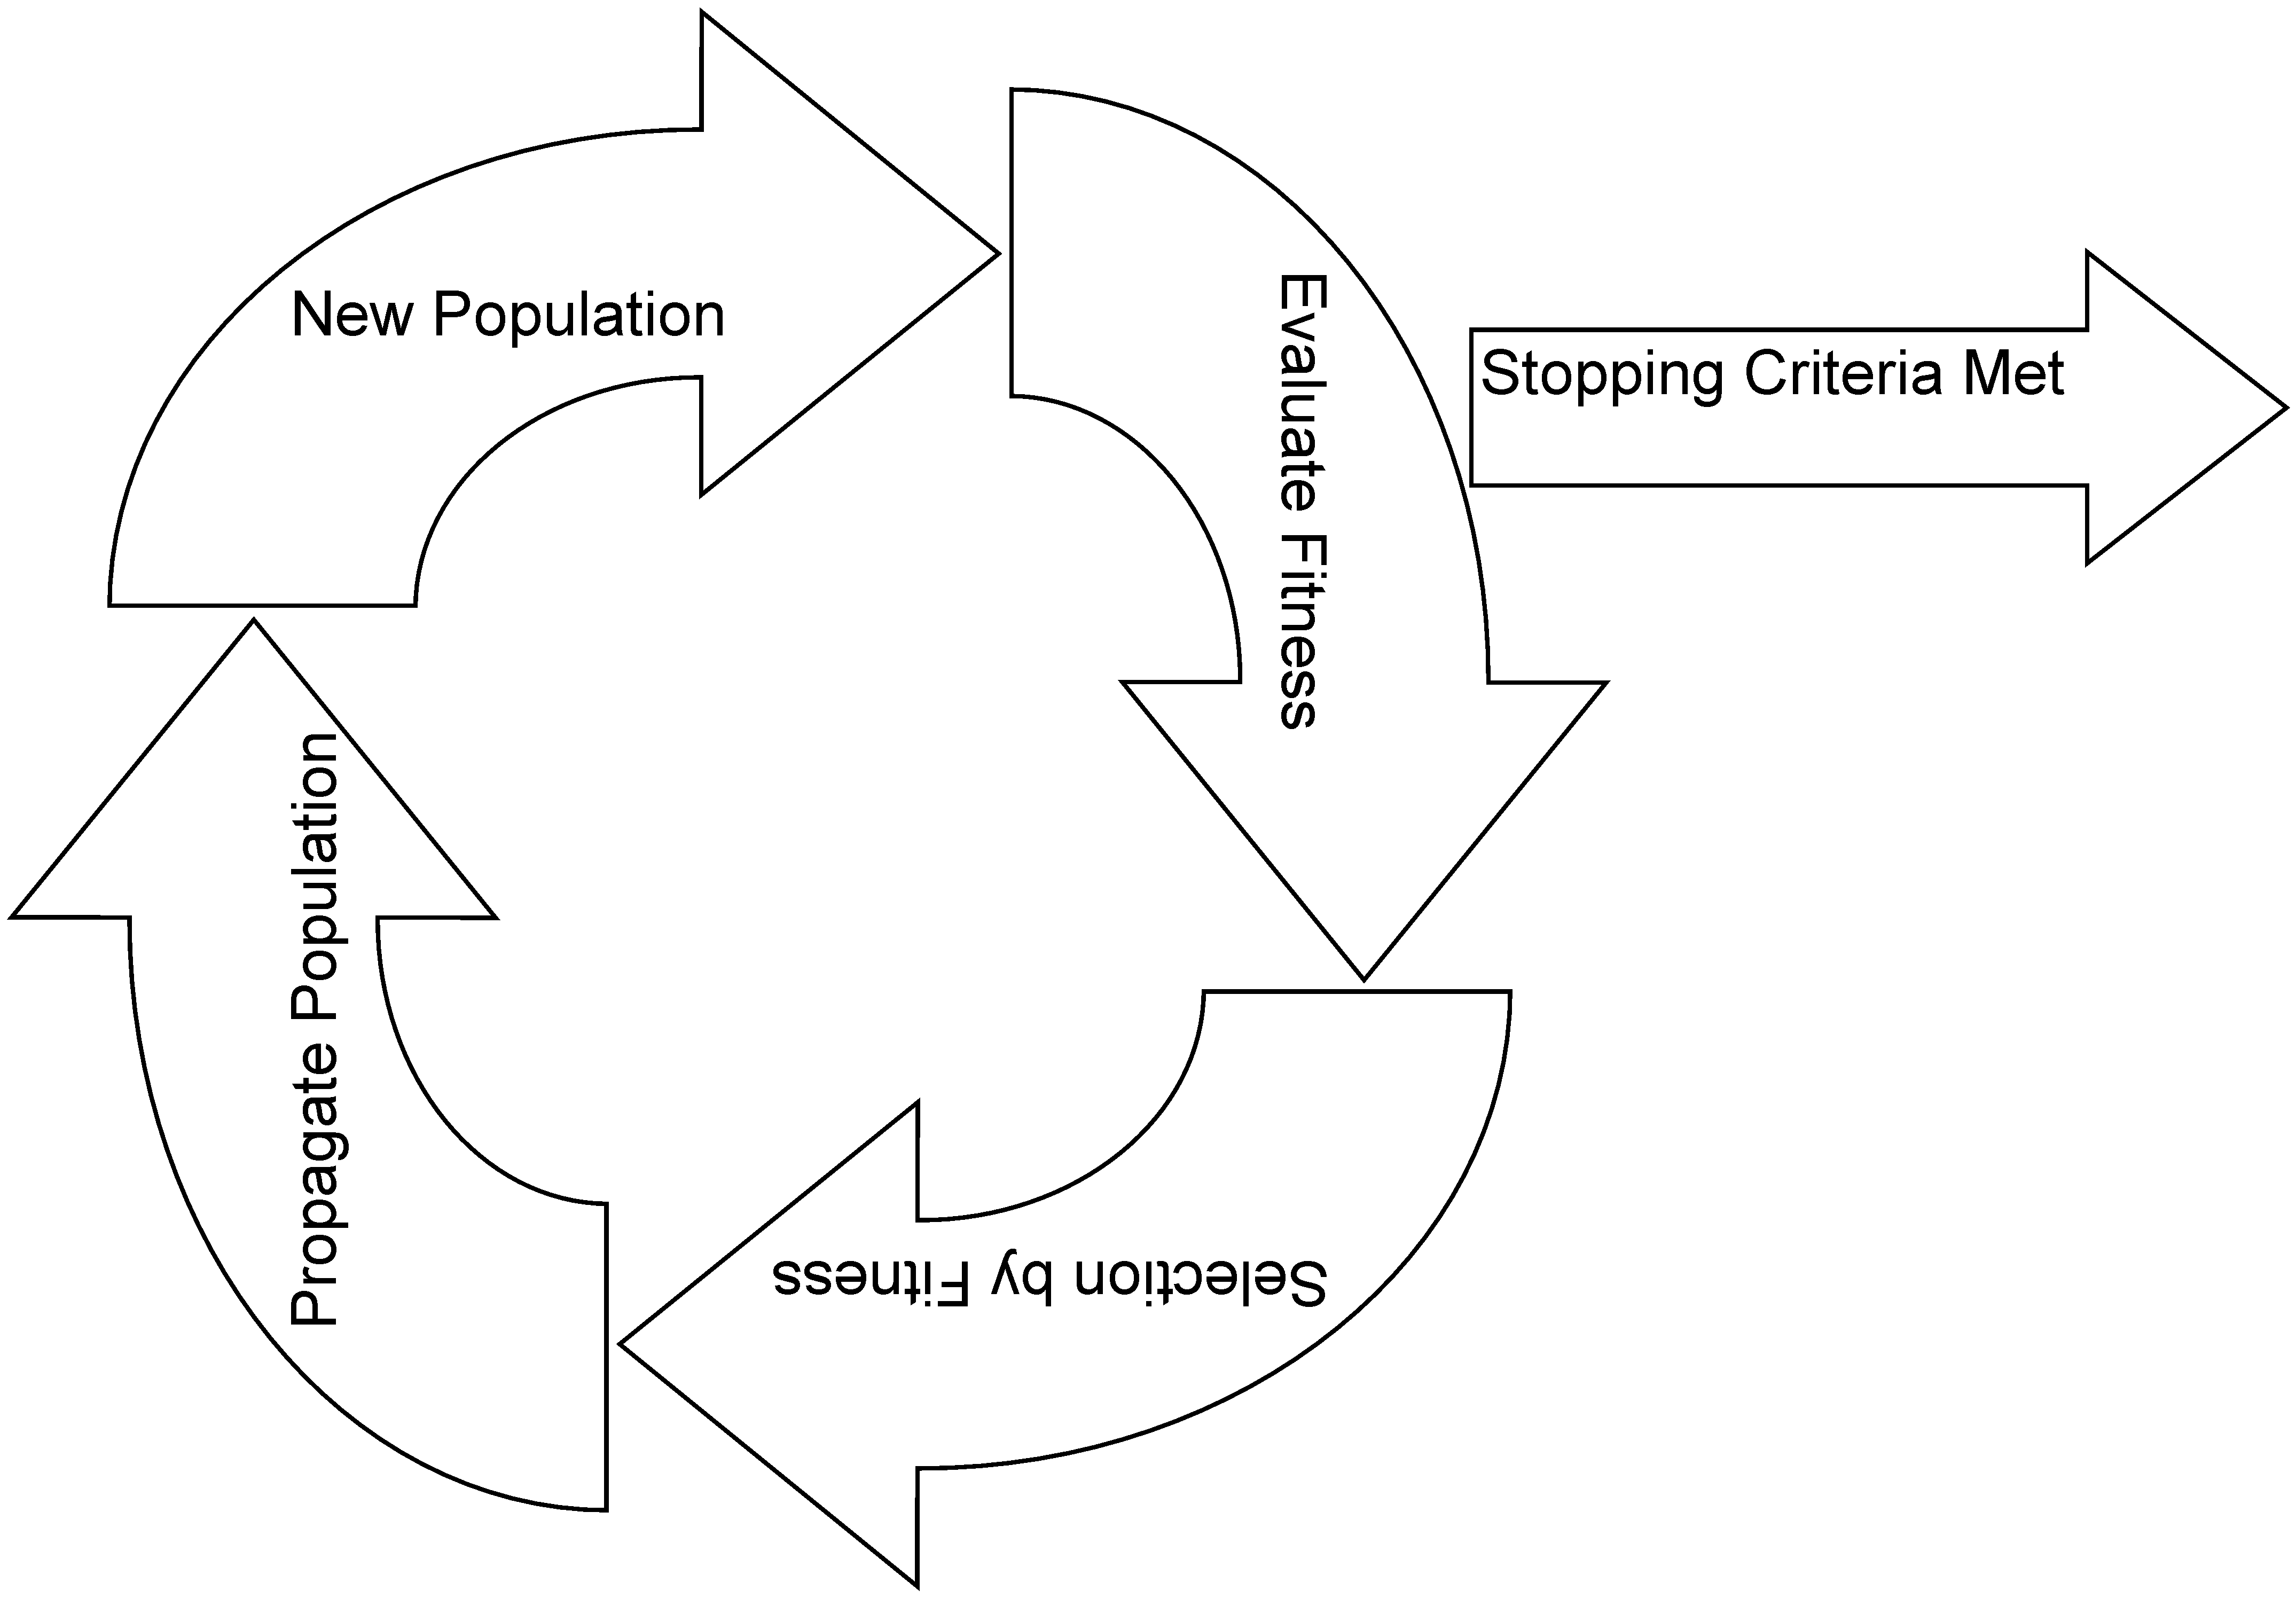
\includegraphics[width=1.0\columnwidth]{Figures/GAFlow.png}}
\caption[Genetic Algorithm Flow]{The general flow of a genetic algorithm. For a
computational genetic algorithm, the process is entered with New Population.
The fitness of the population is then evaluated. If the stopping criteria is
reached, the process is exited. Otherwise, individuals are selected for
propagation based on their fitness. A new population is propagated from
selected individuals using various techniques and a new population is created.}
\label{figure-gaflow}
\end{figure}

\subsection{New Population}

Applying a genetic algorithm to a problem requires that a solution to the
problem can be encoded into a data structure. A single data structure is
referred to as a chromosome. A given chromosome represents a single individual
in the population. In its simplest form a chromosome might consist of a binary
string, that is, a string of 1s and 0s~\cite{Holland1992,goldberg1989genetic}.
The interpretation of the chromosome is problem dependent. If the problem domain
is creating a melody, the 0s and 1s in the chromosome might encode specific
notes and other musical features; if the problem domain is the traveling
salesman problem, substrings in the chromosome might represent the cities that
are visited; if the problem domain is the set of moves in a game, substrings in
the chromosome might represent a particular game move.

The genetic algorithm for any problem begins by initializing the chromosomes
that represent solutions. This is usually done by randomly generating the data
in the chromosome. An individual chromosome is often referred to as an
individual and the complete set of chromosomes is referred to as the population.

The size of the population is an important decision in applying genetic
algorithms to a problem. A population that is too small may not find a solution,
or may take a long time to find a solution, which is a waste of computing
resources. A population that is too large may find a solution, but may use more
resources than is necessary.

\subsection{Fitness}

After a population of solutions is encoded, the next step is usually to measure
the fitness of the solution. Some kind of function is applied to each
chromosome, and the value of the function becomes the fitness of the 
chromosome~\cite{haupt2004practical}.

If the problem domain is creating a melody, the fitness function might be a
comparison of the melody encoded by the chromosome to the desired melody (which
is an objective fitness function) or it may be a human subjective judgement of
the melody; if the problem domain is the traveling salesman problem, the fitness
function would be the length of the tour encoded by the chromosome; if the
problem domain is the set of moves in a game, the fitness function could be the
payoff for making the move specified by the chromosome.

\subsection{Stopping Criteria}

After fitness is measured, the algorithm evaluates whether to stop or not. One
can stop after finding an exact solution, after solutions stop improving, or
after a set number of generations~\cite{dejong2006evolutionary}.

Obviously, if the algorithm has found an exact solution to a problem, there is
no point in proceeding further. This is often the case when optimizing a
mathematical function. If one knows ahead of time that the minimum or maximum of
a function is a particular value, and a genetic algorithm finds a solution that
produces that minimum or maximum, and if there is no reason to search for
additional solutions, the algorithm can terminate.

More often, though, the optimal fitness value is not known a priori. In this
case, one can measure the improvement in fitness between generations and stop
the algorithm when the solutions stop improving or when the improvement in
fitness between generations drops below some threshold.

A third criterion for stopping a genetic algorithm is when a preset number of
populations have evolved. Computer resources can be constrained, and although
an algorithm might find the optimal solution given enough CPU time, one can 
decide before starting the algorithm to terminate after \(n\) generations, and
take the best solution at that point.

\subsection{Selection}

After fitness is measured, the fitness is used to guide the selection of
individuals for propagation into the next
generation~\cite{haupt2004practical,dejong2006evolutionary}.

One method for performing this is to assign a weight to each individual
equal to the ratio of the individual's fitness to the total fitness of the
population. Then each individual is selected with probability equal to that
ratio. This is commonly referred to as roulette wheel selection. Another
technique is to randomly pick two individuals and compare their fitness; the
individual with the higher fitness is then selected. This is referred to as
tournament selection. 

Individuals that are selected can be moved directly into the next generation.
Alternately, they can be combined with other individuals to create new
individuals for the next generation. Either or both of those occur in the
propagation phase.

\subsection{Propagation}

Propagation of the current population usually occurs in conjunction with the
selection phase. The most common methods for creating a new population from the
current population are reproduction, recombination, and
mutation~\cite{goldberg1989genetic,haupt2004practical,DeJong:1989:UGA:93126.93172}.

In reproduction, individuals are copied from the current population directly
into the new population. This might consist of choosing the highest quality
solutions and copying them (elitism) or individuals might be chosen in the
selection phase for copying.

In recombination, two individuals are chosen in the selection process, and then
these two individuals are recombined in some way to create new child
individuals. The most common method of recombination is known as crossover. For
crossover, two individuals are selected and then a position in the chromosome is
randomly chosen, the chromosome is split at that point, and then one of the
sections created is exchanged with the same section in the other chromosome.
This creates two new individuals in the new population. There are other
techniques for recombination; those will be discussed in
Section~\ref{2-recombination}.

In mutation, an individual is selected and the chromosome of the individual is
randomly changed. This can be an individual in the current population; the
mutated individual is then placed in the new generation. Alternately it can be
one of the child individuals created through recombination that is mutated.

After the new population is created, the process repeats.

\section{Genetic Algorithm Extensions}

A large amount of research has been conducted into extending various features of
the basic algorithm to cover a larger number of problems. We briefly look at
some of those extensions here, with additional coverage of specific fitness
measurement extensions in Chapter~\ref{chap:background}.

\subsection{Chromosomes}

The chromosomes in genetic algorithms were introduced above as a binary string.
However, the chromosome is, more generally, some data structure that represents
the solution to some problem. So one can have chromosomes that are strings or
arrays of integers, arrays of real numbers, or strings or arrays of some other
encoding~\cite{haupt2004practical}. Chromosomes can be structured as trees,
where nodes and leaves represent some part of the solution. These are usually
used in genetic programming where the tree is the parse tree of some computer
program and the objective is to evolve a program~\cite{koza1992genetic}.
Chromosomes can be used to represent graph-like structures such as finite state
machines~\cite{fogel1999intelligence,fogel2000evolutionary}. Linear chromosomes
that are translated into gene expression trees are used in gene expression
programming~\cite{ferreira2012gene}.

\subsection{Fitness evaluation}

The fitness function is used to evaluate the quality of the solution. Thus, it
is better to have some objective function or measurement that can be applied to
the chromosome. When attempting to optimize some mathematical function, that is
easy to do. The chromosome becomes an input to the function, and the objective
measure is simply the function output. For other problems, though, there may not
be an objective function. For example, when applying a genetic algorithm to art
or music, a subjective fitness function is used~\cite{eiben2003introduction}.
For these applications a human is usually used to provide an assessment of the
quality of the solution.

And then there are times when there is neither an objective nor a subjective
fitness function. When applying genetic algorithms to games, especially games
that have a stochastic component, there is no good objective fitness function.
If a chromosome is designed to output moves for a game, how does one know
whether the strategy encoded by the chromosome is a good? Just because an
individual wins a game does not make the individual high quality: it could be a
poor quality individual but played against a worse player. Similarly, just
because an individual loses a game does not make the individual poor quality: it
could have lost just because of chance. In this case, one uses a competitive
fitness function~\cite{fogel1999intelligence}. We discuss competitive fitness 
functions in more detail in Chapter~\ref{chap:background}.

\section{Recombination and mutation} \label{2-recombination}

There are many different ways to perform recombination in a genetic algorithm.
The basic crossover operation was briefly discussed earlier. When recombining
strings or arrays, one can also use multi-point crossover where multiple
crossover points are used. In uniform crossover each gene in the child is
randomly selected from the parents. With real-valued or continuous chromosomes,
there is arithmetic (also known as blended) crossover that linearly combines
both parent chromosomes to create two child
chromosomes~\cite{haupt2004practical}. With a problem like the traveling
salesman problem, the standard crossover operations are not appropriate since
they can duplicate cities in the chromosome. For permutation type problems like
the traveling salesman problem, other crossover operations have been
developed~\cite{goldberg1989genetic} which avoid duplications in the child
chromosomes.

\clearpage
\chapter{Background Research}\label{chap:background}

\section{Overview}

Research in applying evolutionary computation to games\footnote{The term
``game'' is highly overridden. Throughout this chapter (and the entire thesis)
the term generally refers to board games or other similar types of competitions
that are played between two or more persons} has been performed almost since the
study of evolutionary computing began. Holland, in his seminal work
\emph{Adaptation in Natural and Artificial Systems}, discussed applications of
genetic algorithms to games~\cite{holland1975adaptation,Holland1992}. Holland
showed that the search space of many games quickly grew to a size that is not
computationally tractable. He then discussed how an artificial adaptive system
(i.e., evolutionary computation) could be used to efficiently search the game
space and realize an optimal strategy.

In Chapter \ref{chap:algorithm} the design of the genetic algorithms used for
this research is presented. The decisions made for those algorithms have a basis
in research that applied genetic algorithms to the study of various games. In
the remainder of this chapter we review some of that research.

\section{Deterministic zero sum games}

One fundamental type of game is the deterministic two player game with perfect
information. To be deterministic means that the game has no element of
randomness or chance in it. Two player obviously means that only two players are
involved in the game. (Using only two players is done to make computations easy,
but the results are easily extended to games with more than two players.) A two
player game involves a gain or payoff to one player and a loss to the other
player. The gain and loss are not necessarily equal; when the gain to one player
is equal to the loss experienced by the other player in the game, the game is
known as a zero sum game. In its simplest form the payoff is a binary win/loss
result: one player wins and the other player loses. Finally, for a game to
involve perfect information means that every player in the game knows everything
about every the other player's state and future possible moves.

\subsection{The Prisoner's Dilemma}

One of the most studied deterministic two player games is the two person game
known as the Prisoner's Dilemma, a game in which two players can either
cooperate or defect, without the ability to communicate with each
other~\cite{Flood1958,Nowak1993,Mittal2009}. The payoff matrix for this game is
shown in Table \ref{table-pdpayoff}. This game is not a zero sum game.

\begin{table}[h]
\caption{Payoff matrix for Prisoner's Dilemma}
\begin{center}
\begin{tabular}{|l|c|c|}
\hline
\multicolumn{1}{|l|}{{Decision\!}}
& \multicolumn{1}{|c|}{Cooperate}
& \multicolumn{1}{|c|}{Defect} \\ \hline
Cooperate &  R,R & S,T \\ \hline 
Defect    &  T,S & P,P  \\ \hline \hline
Notes & \multicolumn{2}{|c|}{\(T > R > P > S\)} \\ 
      & \multicolumn{2}{|c|}{\(2R > T + S\)} \\ \hline
\end{tabular}
\label{table-pdpayoff}
\end{center}
\end{table}

%\multicolumn{1}{|l|}{\raisebox{-1.50ex}[0cm][0cm]{Decision\!}}

In a single iteration of this game, the best strategy for both players is to
defect~\cite{nash50,Nash1951}. Suppose player 1 chooses to cooperate;
looking at the payoffs, this player sees that regardless of which strategy the
opponent chooses, player 1 gets a better score by switching to defect. The same
reasoning applies to player 2.

However, studies have shown that when the game is played repeatedly (known as
the Iterated Prisoner's Dilemma game), a strategy of cooperation will
spontaneously evolve within a population~\cite{Axelrod1984, Nowak1993,
DBLP:conf/cig/QuekG07, Mittal2009, WangTao2010}. This game is different from the
others presented below in that there is an objective measure of fitness for this
game. For Nowak and Sigmund, ``Strategies with higher payoffs produce more
offspring~\cite{Nowak1993}.'' Similarly for Quek and Goh, ``\ldots fitness
assignment is performed after each tournament and is given by the payoffs
accumulated throughout the game play~\cite{DBLP:conf/cig/QuekG07}.'' Mittal and
Deb studied the Prisoner's Dilemma as ''\ldots a bi-objective optimization
problem of maximizing the player's own score and simultaneously minimizing the
opponent's score'' where the score was the sum of the player's payoff over the
set of games~\cite{Mittal2009}. Wang, et al., also used the sum of payoffs as a
fitness measure~\cite{WangTao2010}.

In other games, having an objective fitness measure is not always possible. In
some games the only thing that can be measured is which player won the game and
which lost; but the winner does not necessarily have high fitness and the loser
does not necessarily have low fitness. A mediocre player could get a large
number of wins if many of the opponents are worse players. In these cases, a
competitive fitness function is used. In the remainder of this section we look
at several studies that used competitive fitness functions.

\subsection{Tic-Tac-Toe}

The game of Tic-Tac-Toe is a relatively simple two-player competitive game
played on a 3x3 grid. Players alternately place a symbol, (usually one player
plays X and the other plays O) on an open grid space; the winner is the player
that manages to create a straight line (vertically, horizontally, or diagonally)
of three symbols. Fogel showed that genetic algorithms could be used to evolve
neural networks to play the game~\cite{Fogel1993}.

Fogel played a population of 50 randomly generated neural networks against a
rule-based opponent which also had a small probability of making a random move.
Each neural network played 32 games against the rule-based player. A competitive
fitness function was used in which the neural network was awarded +1 for
winning, -10 for losing, and 0 for a draw. Because of the element of randomness,
a neural network with a high score did not necessarily have a perfect strategy.
That is, a neural network could have a high score because the opponent made
several bad moves over the 32 games. So, before propagating the population,
Fogel ran a further competition where a neural network played 10 other randomly
chosen networks. Neural networks that scored high in the second competition were
allowed to reproduce to the next generation.

In this example, the basic elements of a competitive fitness functions are
present: 1) individuals in the population 2) compete against some other player
and 3) are awarded points for winnning, losing, or drawing. In this study, the
individuals in the population competed against static players from outside the
population. However, individuals in a population can also compete against each
other in a process known as coevolution.

\subsection{Checkers}

In Checkers each player has 12 pieces that can move diagonally on a board
divided into an 8x8 grid of squares. If one player's piece is adjacent to the
opponent's piece, and there is a blank square on the opposite side of the
opponent's piece, the player can jump that piece and remove the opponent's piece
from the board. The winner is the player who removes all of the opponent's
pieces from the board. Fogel and Chellapilla used evolutionary computing  to
evolve neural networks that could generate moves for the
game~\cite{Fogel2000Anaconda,journals/tec/ChellapillaF01}. 

Interestingly, Fogel's genetic algorithm did not use any reproduction operators
on the genome. The genome was evolved by picking the fittest genomes to carry
over to the new generation, with new genomes created by mutation only.

Fogel and Chellapilla used a competitive fitness function for their research.
A population consisted of 15 parents from which 15 children were created by
mutation. Each neural network in the population then played five games against
five other randomly chosen neural networks from the population. Wins, losses,
and draws were awarded +1, -2, or 0 points respectively. After all games had
been played, the top 15 neural networks by total score were copied into the next
generation and the process was repeated. Again, neural networks with high scores
were not necessarily the best players, since a high score could be obtained by a
player with poor strategy if the opponents of the player were all worse players.
To validate their results, Fogel and Chellapilla took the best evolved neural
network and played it against human players over the Internet. After 250
generations, it played just below expert level, and after 840 generations their
evolved ANN player was able to play at Expert level, well above the average
human player.

This is an example of coevolution. In this work the competitive fitness function
consists of individuals competing against other individuals in the same
population. However, each individual only competes consists of a subset of the
population.

\subsection{Othello}

Othello (also known as Reversi) is a two-player game where players take turns
placing colored tokens on the board. The winner is the player who can get the
most tokens of his color on the board. Play is complicated by the fact that a
player can only place a token in a way that ``captures'' the opponent's tokens.
This is done by placing a token adjacent to an opponent's token such that at
least one of the opponent's tokens lies between the new token and one of the
already placed tokens. When a player captures a line of the opponent's tokens,
all of the opponent's tokens in that line change to the capturing player's
color. Chong et al., investigated evolving the evaluation function of a neural
network to create an ANN that could play Othello~\cite{ChongTW05}.

The population consisted of 10 parent neural networks, with 10 children created
through mutation. Each of the 20 individuals in the population then played 5
games against other neural networks chosen randomly from the population. Wins
were awarded five points, losses received zero points, and draws resulted in
each network getting one point. The top ten scoring individuals were propagated
to the next generation as parents. At each generation, a second evaluation was
performed by having the best neural networks play against a computer player that
used a deterministic evaluation function to generate moves. These secondary
competitions were only used to evaluate the ability of the neural networks, and
were not used to guide the evolution. As the population evolved, competition
against the computer player showed that the neural networks were indeed playing
at higher levels, achieving master level at about the 800th generation.

This example of coevolution is very similar to the previous example.

\subsection{State Space Complexity}
We could continue to cite other research into genetic algorithms and games, and
will make a brief mention below. But at this point it will be instructive to
look at the state space complexity of games. The first four games cited above
were introduced from the least complex to the more complex.

The state space complexity of these and other games is well known and can be
easily found (or calculated). Allis, for example, provides the following
estimates for several games including some of the ones\footnote{Allis looked at
games from the Computer Olympiad (see
\url{http://www.grappa.univ-lille3.fr/icga/competition.php?id=3} which does not
include The Prisoner's Dilemma. However, the state space for The Prisoner's
Dilemma is easy to calculate. With a single iteration, each player has two
possible moves, so the state space complexity is \(2\cdot2=4\). If iteration is
allowed, then with two iterations each player has four moves and the state space
complexity is 16. Three iterations gives a state space complexity of 64. In
general, the state space complexity is \(2^{2n}\) where \(n\) is the number of
iterations.} discussed above~\cite{Allis1994}. Tic-Tac-Toe has an estimated
state space complexity of \(\approx10^{3.7}\). The state space complexity for
Checkers is \(\approx10^{18}\). As might be expected, Othello is more
complicated with a state space complexity of \(\approx10^{30}\). Even for games
of much higher complexity, genetic algorithms have been used with success. While
not able to provide a complete solution, genetic algorithms have been applied to
some subproblems for games such as Chess~\cite{Mitsuta:2010:OPG:1994486.1994517}
(state space complexity of \(\approx10^{50}\)) and
Go~\cite{shah2012Go,Blackman2009Go} (state space complexity of
\(\approx10^{172}\)). It is clear that the state space complexity of a game is
not a barrier to the use of evolutionary computing.

These numbers will become important in Chapter~\ref{chap:algorithm} where the
state space complexity of Monopoly is discussed.

Deterministic, two-player, zero-sum games are widely studied because they are
relatively simple to understand and play. Many classic game theory games like
Prisoner's Dilemma have very small state spaces. Some of them have a relatively
small search space (Othello, Chess and Go being obvious exceptions), which makes
them tractable to study and simulation. However, there is a whole class of games
with many examples that are non-deterministic, multi-player (but still usually
zero-sum) games.

\section{Non-Deterministic games}

Non-deterministic games are those that have some element of randomness in them.
Many gambling games such as poker, blackjack, roulette, or craps are based
on random outcomes. Randomness in those games is provided by the shuffling of
cards, the spin of a wheel and roll of a ball, or the throw of dice. Many
recreational board games use dice or cards to provide a random element to the
game. 

While not as well studied as the two player games mentioned previously, there
has been some research on using evolutionary computation to create winning
strategies for non-deterministic games. In this section we look at three games
to which evolutionary computing has been applied: Rummy, Acquire, and Monopoly.

\subsection{Acquire: Evolving Board Evaluation Functions for a Complex Strategy
Game}

Acquire is a board game in which players attempt to gain wealth by building and
investing in properties\footnote{See \url{http://en.wikipedia.org/wiki/Acquire}
for details}. The player with the most wealth at the end of the game is the
winner.

Anthony applied genetic programming (a subset of evolutionary computing) to the
problem of evolving board evaluation functions for the game~\cite{Anthony2002}.
She identified two basic decisions a board evaluation function would need to
make for the game: where to place a tile (build a property) on the board and
which property to invest in. 

Like many other games, there is no objective fitness criteria for Acquire, so
Anthony used a competitive fitness function. She evaluated several possible
methods for computing a game score including number of wins, amount of money
earned, and ratio of money earned in a game to total amount of money earned by
all players in the same game. The last method was the one used in her
experiments.

There were 1000 players in a generation, and 50 generations were evolved. Each
player in a generation played 10 games against other players in the population.
The raw score was computed for each game, and the average over 10 games was the
player's fitness for that generation. To validate that the population was
evolving better evaluation functions, the best player in the final generation
was played against the best player in each previous generation.

\subsection{Strategies for the Game of Monopoly}

The last game we look at in this section is the game of Monopoly, which is the
subject of this research. A detailed overview of the game is presented in
Chapter~\ref{chap:monopoly}, but it will be helpful to understand a few basics
about the game here. 

In the game of Monopoly, players can purchase specific locations on the game
board. Some of those locations are known as streets, and streets are further
grouped into one of eight color groups (See Figure~\ref{figure-monoboard}). When
a player lands on a location owned by another player, the first player pays rent
to the owner. If a player owns all the streets in a color group, the player can
build houses or hotels which dramatically increases the rent.

\subsubsection{Monopoly as a Markov Process}

Some of the first studies of the game were statistical analyses of which
locations were more valuable to own. Ash and Bishop modeled the Monopoly board
as a Markov process~\cite{Ash1972}. From this they concluded that the properties
with the greatest expected income where streets which comprise the Green group
on the east side of the board, followed by the two groups (Red and Yellow) on
the north side of the board.

Abbott and Richey extended Ash and Bishop's work with a more
rigorous\footnote{In 1972, Ash and Bishop did not have the same computing
resources to apply their calculations that Abbott and Richey had in 1997}
examination of the game as a Markov process~\cite{Abbott1997}. They came to a
similar conclusion: the expected income is greatest from the Green group,
followed by Red, Yellow, and Orange. However, because it costs much less to
build houses and hotels on the Orange group, the more valuable group is Orange,
followed by Red, then Yellow.

\subsubsection{An Evolutionary Approach to Strategies for the Game of Monopoly}

Frayn used evolutionary computing to develop a strategy for property valuation
and property management~\cite{DBLP:conf/cig/Frayn05}. Frayn used four different
chromosomes for each individual in the population. Three of the four chromosomes
represented the values of properties that could be owned by players. Each gene
in those chromosomes represented the value of a particular property. The fourth
chromosome represented other game decisions such as when to mortgage a property,
or the minimum amount of cash a player should retain.

Frayn came to the conclusion that the best property group was the Orange group.
In contrast to the conclusions of the previous two studies, the best individuals
in Frayn's experiment avoided the Red, Yellow, and Green groups. His experiment
also found that the properties on the south and west sides all had values
greater than their costs, whereas everything on the north and east sides had
values less than their costs. His individuals were thus buying the properties on
the south and west sides, and avoiding properties on the north and east sides.

Frayn used a genetic algorithm with 1000 players in a generation, and
1420 generations were evolved. He used a competitive fitness function where each
player in a generation played 100 games against three other players in the
population. The winner of the game received a score of +3 points, second place
recieved +2 points, third place received +1 point, and fourth place received 0
points. The total fitness was the sum of points over 100 games.

\subsubsection{Property Trading Strategies} \label{3_trading}

Yasumura, Oguchi, and Nitta, studied different negotiating strategies to
identify the best way to conduct negotiations between
players~\cite{Yasumura2001Negotiate}. They constructed an evaluation function
that was the summation of property values under different ownership conditions,
less expected losses over the short term (1 dice roll) and medium term (1 trip
around the board). The summation and losses were each also weighted by constant
terms that were varied to make strategies more bullish (more weight to potential
gains and more likely to trade a property) or bearish (more weight to expected
losses and more likely not to trade a property). They found that a strategy
where the gains and losses in their evaluation function were weighted evenly
gave the best results.

\section{Competitive Fitness Functions}

When used in optimization problems, genetic algorithms usually rely on an
objective fitness function. However in the particular case of games, there is no
objective way to measure fitness, and so as seen previously in this chapter a
competitive fitness function must be used. In this section we review some of the
research into competitive fitness functions.

\subsection{Competitive Environments Evolve Better Solutions for Complex Tasks}

Angeline and Pollack conducted an early study into competitive environments for
evolutionary computing. They claimed that ``\ldots for many complex tasks an
independent fitness function is either impractical or impossible to
provide.~\cite{Angeline:1993:CEE:645513.657590}'' Their research attempted to
demonstrate that fitness functions that are dependent on the constituents of the
population ``\ldots can provide a more robust training environment than
independent fitness functions.~\cite{Angeline:1993:CEE:645513.657590}''

In their paper they discussed three different ways to structure a competitive
fitness function.

First, they looked at a round robin style of tournament where every member of
the population engages in a competition with every other member of the
population. In Axelrod's study of the evolution of cooperation in Prisoner's
Dilemma, every member of the population played every other member of
the population~\cite{Axelrod1984}. Of course, if the size of the population is
\(n\), the number of competitions is of order \(O(n^2)\), so this is not
very scalable.

Second, they looked at a bipartite competitive environment. In this environment
every individual in one population competes against some individual in another
population. This type of competition was used in a study of sorting networks by
Hillis~\cite{Hillis:1990:CPI:87498.87560}. Hillis had two populations: one
population consisted of sorting networks, and the second population consisted of
sets of test cases, where each set is an individual. Each sorting network
competed against one set of test cases. The fitness of each sorting network was
scored based on the percent of test cases that were sorted correctly; whereas
each set of test cases was scored based on the percent of test cases that were
not sorted correctly. This type of fitness environment requires \(n\)
competitions for a population of size \(n\).

Finally they looked at a single elimination tournament style of
competition within a single population. In this style of competition, pairs of
individuals are randomly selected from a population and engage in a competition.
The winner is returned to the population, the loser is temporarily removed from
the population. This proceeds until a single individual remains. The fitness of
each individual is the number of competitions that the individual won. This
requires \(n-1\) competitions for a population of size \(n\).

Angeline and Pollack found that the tournament fitness function performed well
in evolving players for the game of Tic-Tac-Toe. The tournament fitness function
has several advantages over other fitness functions: it does not require task
knowledge of the optimization problem as an objective fitness function might;
and it avoids the need to develop a separate population and fitness function as
the bipartite competition does.

\subsection{A Comparative Study of Two Competitive Fitness Functions}

Panait and Luke provided a further examination of tournament selection versus
round robin style competitions~\cite{Panait02acomparative}. In their study they
used both tournament selection and generalized round robin competition on four
different problems: two versions of the game Nim, the Rosenbrock function, and
the Rastrigin function\footnote{Like other functions used in the study of
optimization, the Rosenbrock and Rastrigin functions have many local minima and
a single global minimum. For examples see
\url{https://en.wikipedia.org/wiki/Rosenbrock_function} and
\url{https://en.wikipedia.org/wiki/Rastrigin_function}}.

Panait and Luke presented a generalized version of round robin called K-Random
Opponents. When \(K=1\), K-Random Opponents is a single elimination
tournament: the population is divided into pairs and each pair engages in a
single competition with the loser eliminated from further competitions in that
generation. This is used when the cost of a single competition is relatively
high and thus it would be impractical to perform a full round robin tournament.
When \(K=n-1\), a complete round robin tournament is conducted where every
member of the population engages in one competition against every other member.
When \(1 < K < n-1\), each individual competes against \(K\) opponents.

For each of the four problems they evaluated, Panait and Luke found that in
general, the Single Elimination Tournament performed better than K-Random
Opponents for almost any value of K. The specific cases where Single Elimination
Tournament performed worse than K-Random Opponents was when noise was introduced
into the fitness calculation. Noise was introduced by taking a random number of
competitions and exchanging the scores of the two players. That is, for a random
percentage of games, the loser of the game is awarded a win, and the winner is
given the loss. Luke and Panait found that Single Elimination Tournament
performed worse than K-Random Opponents for some values of \(K\) when the noise
percentage was greater than 30\%.

The research cited above into Checkers, Othello, Acquire, and Monopoly all used
K-Random
Opponents~\cite{Fogel2000Anaconda,journals/tec/ChellapillaF01,ChongTW05,Anthony2002,DBLP:conf/cig/Frayn05}.

\subsection{Fitnessless Coevolution}

More recently Ja\'{s}kowski, Krawiec, and Wieloch realized that when a
competitive fitness function was being used as part of a genetic algorithm, one
could skip the fitness evaluation component and use the competitions directly in the
selection phase of the algorithm~\cite{Jaskowski:2008:FC:1389095.1389161}. 

When using fitnessless coevolution, the fitness evaluation step is skipped
completely. The genetic algorithm then proceeds to the selection phase where
individuals are selected for propagation to the next generation, either
directly, or as part of reproduction. For each new individual in the next
generation, a sample set \(S\) of individuals is selected with replacement from
the current generation. The individuals in \(S\) then compete in a single
elimination tournament and the winner of the tournament becomes a candidate for
being directly added to the next generation, or becoming a parent of a new
individual in the next generation. The size \(t\) of sample set \(S\) can be
varied. If \(t=1\), fitnessless coevolution is the same as Single
Elimination Tournament.

Ja\'{s}kowski, Krawiec, and Wieloch evaluated fitnessless coevolution against a
similar set of problems as Panait and Luke (a single version of Nim, the
Rosenbrock function, and the Rastrigin function) and additionally tested it with
Tic-Tac-Toe. They found that fitnessless coevolution was competitive with Single
Elimination Tournament and K-Random Opponents. It usually outperformed Single
Elimination Tournament, and like Single Elimination Tournament only performed
more poorly than K-Random Opponents when there was a noise percentage more than
30\%. It simplifies the competitive fitness genetic algorithm by eliminating
numerical fitness and the evaluation phase of the genetic algorithm. Also,
fitnessless coevolution works best with tasks that satisfy the transitivity
condition: in a game, if \(Player_{i}\) beats \(Player_{j}\) and \(Player_{j}\)
beats \(Player_{k}\), then \(Player_{i}\) beats \(Player_{k}\) for all i, j, k.

However, while fitnessless coevolution simplifies the genetic algorithm by
eliminating numerical fitness, this can also be a disadvantage. In many of the
studies discussed above, the best individuals in a generation were often
validated by competing them against some other benchmark player, either a
different AI opponent or a human competitor. With no numerical fitness, it is
more difficult to select the fittest players in a generation for the objective
competition.

\section{Summary}

Evolutionary computing has been applied to the study of games for many years. It
has been used successfully for the very simplest of games to the most
complicated of games. When genetic algorithms are applied to games, it is almost
always necessary to use a competitive fitness function. Researchers generally
use K-Random Opponents as the competition structure. If the game has a very high
time- or space- complexity they may use a single elimination tournament
style of competition \(K=1\). Even if the game has low complexity, in the
absence of noise, single elimination tournament style competitions appear to
provide the most robust fitness determination. However, if there is a lot of
noise, single elimination tournament does worse than K-Random Opponents with a
higher value of K. This is because noise can distort the results of a single
competition and multiple competitions are needed to smooth out the effects of
noise.
\clearpage
\chapter{Overview of the Game of Monopoly}\label{chap:monopoly}

Monopoly is a game where players traverse a path around a board on which most
spaces represent a property which players can buy (See 
Figure~\ref{figure-monoboard}). Other players must pay ``rent'' to the owner of
a property when they land on that property.

\begin{figure}[htp]
\centerline{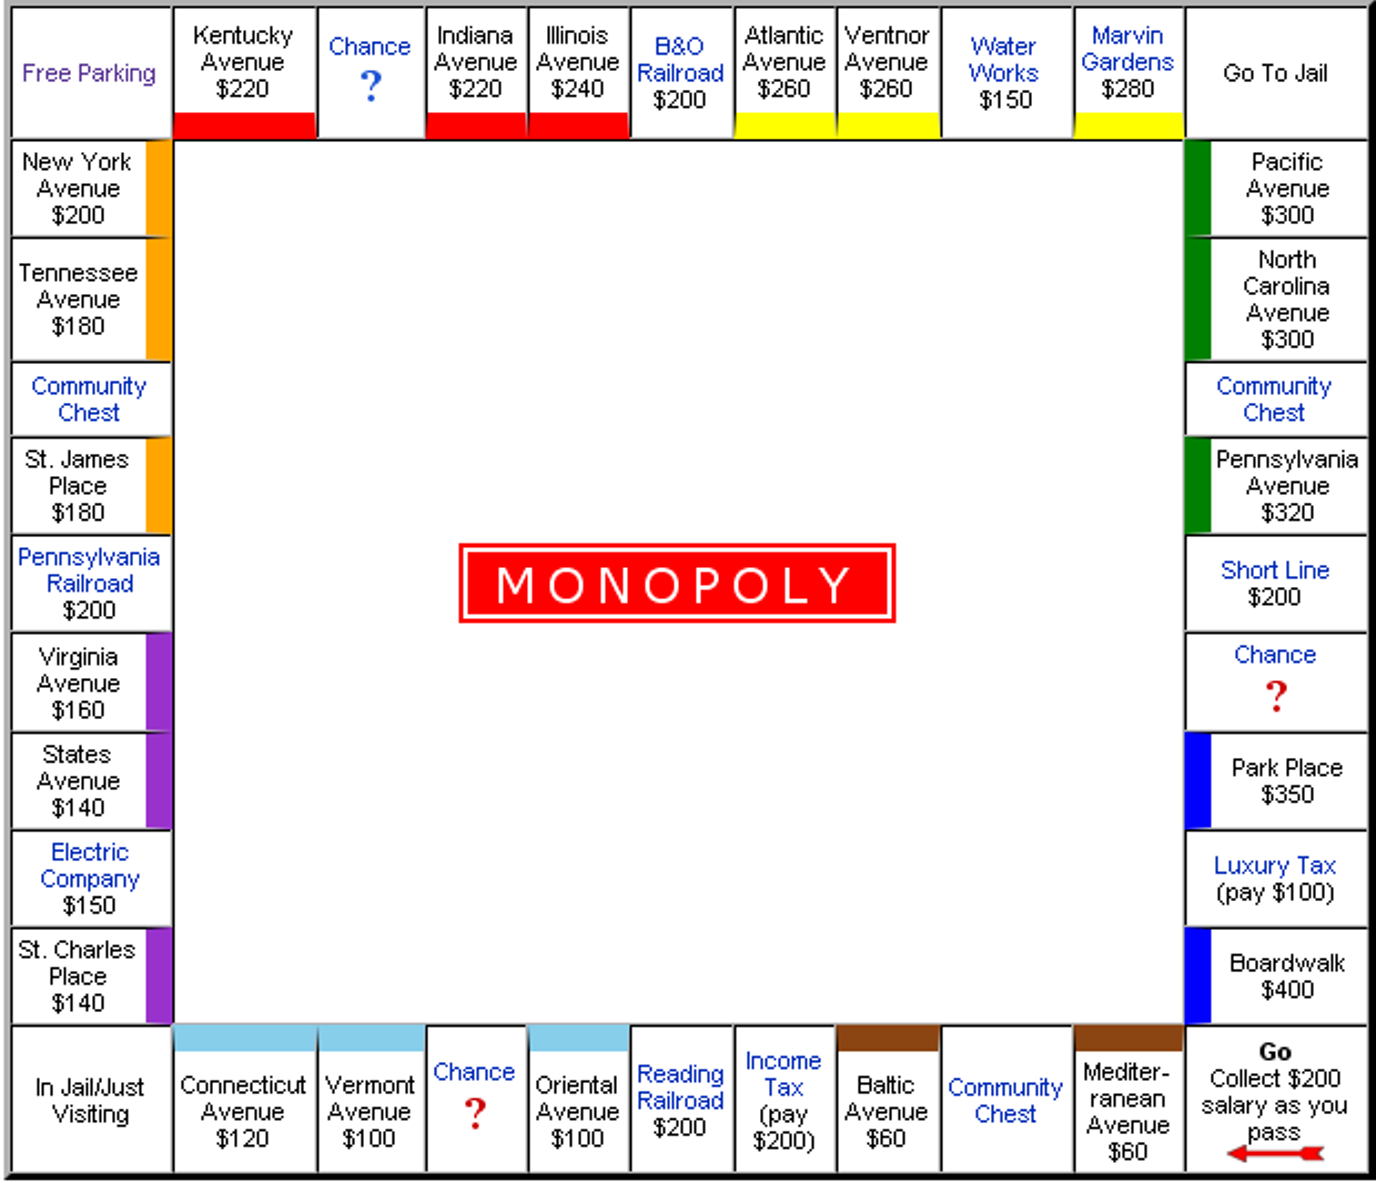
\includegraphics[width=1.0\columnwidth]{Figures/Monopoly.png}}
\caption[Board layout for Monopoly]{The board layout for Monopoly. For this
study, the edge of the board containing ``Go'' through ``Connecticut Avenue'' is
south. Proceeding clockwise, the next edge is west. The top of the figure is
north. The final edge of the board is east. South includes the cheapest
properties; east contains the most expensive. Monte Carlo simulations of dice
rolls show that the most landed on locations are on the west and north edges of
the board.}
\label{figure-monoboard}
\end{figure}

When one player owns all the properties in a color group (a monopoly), the
player can ``develop'' the properties by building houses or hotels. This
increases the rent value which increases the probability that an opponent will
not be able to pay the rent. If a player cannot pay rent, the player must sell
or mortgage properties, and if that is not possible, give their properties to
the owner. The winner is the player who bankrupts the other players.

Another important feature of Monopoly is the ability of players to trade
different properties. Because of the random nature of a player's moves, it is
improbable that a single player will be able to land on and buy all the
properties in a group. So, players usually must trade with other players to gain
a monopoly on a property group. 

\section{Movement}
Players take turns moving around the game board based on the roll of two dice.
Thus, for each move, the player will move between 2 and 12 spaces. The player's
location on the board is represented by a token.

If a player rolls doubles (the two dice have the same value), the player is
allowed a second roll of the dice. If the player rolls doubles on the second
roll, the player is allowed a third roll. If the player rolls doubles a third
time, they must move their token directly to Jail.

\section{Game locations}
There are 28 locations on the game board that can be bought by the players. The
locations are divided into 22 streets, which are further grouped into 8 color
groups, 4 railroads, and 2 utilities. Figure~\ref{figure-street} shows the
property card for a street location.

\begin{figure}[htp]
\centerline{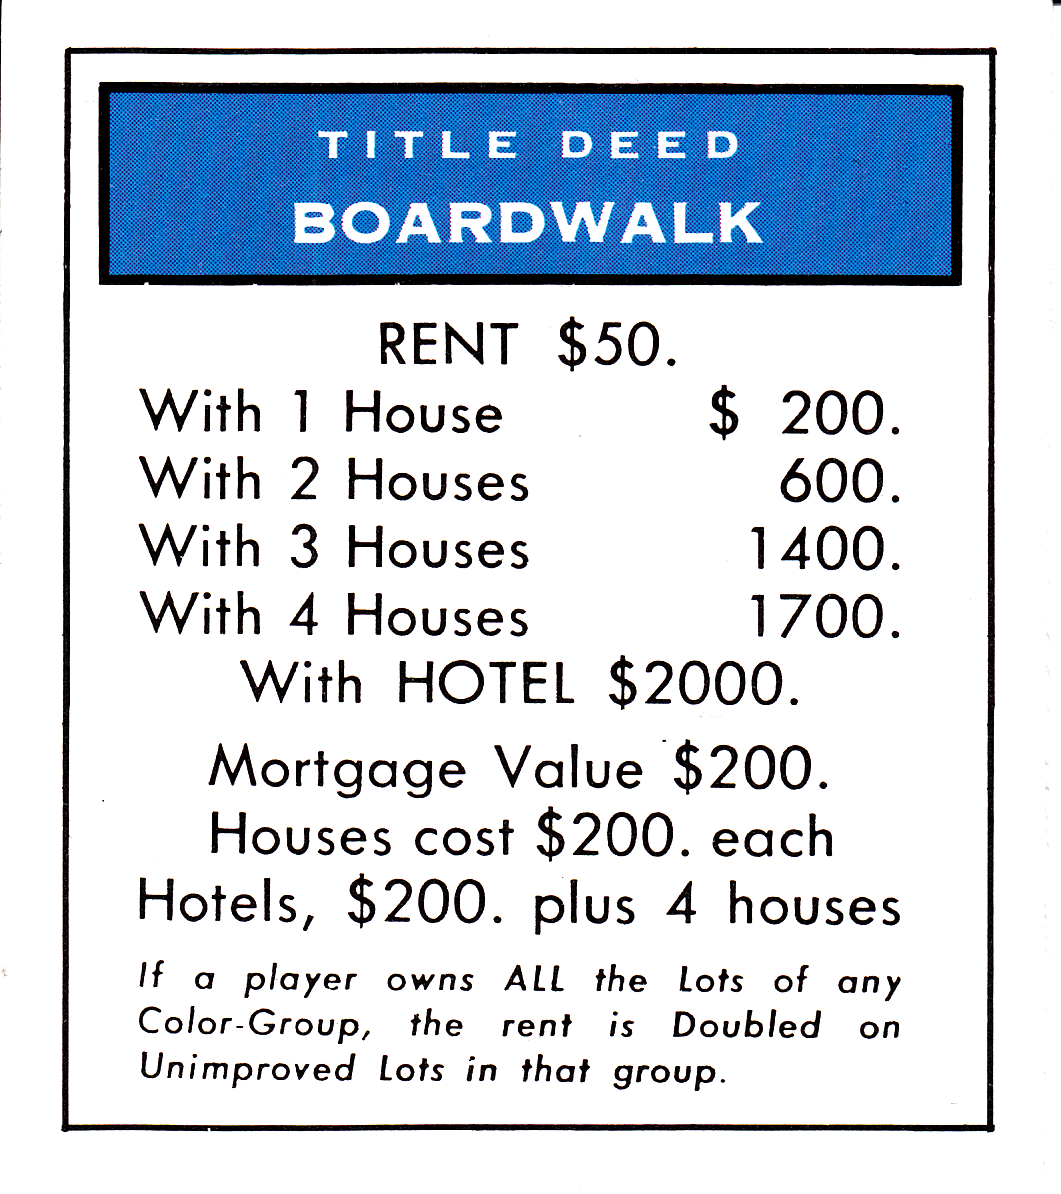
\includegraphics[width=0.5\columnwidth]{Figures/Boardwalk.png}}
\caption[Example property card]{The property card for the street location
Boardwalk. The card lists various costs including how much rent an opponent
pays, the mortgage value of the property, and how much the owner pays to buy
houses or a hotel.}
\label{figure-street}
\end{figure}

If the player lands on an unowned location, the player may buy the property. If
the player declines to buy the property, the property is auctioned among all
players (including the player who originally declined to buy the property).
If the player lands on a property that is already owned, the player must pay
rent to the owning player.

Once a player obtains all properties within a group, the properties can be
``improved'' by building houses or hotels on the property. Improved properties
have a higher rent.

The other 12 locations on the board cannot be owned by any player. For this
study, only one of those locations is important. That location is the corner
space marked ``Jail.'' There are three circumstances that can send a player to
Jail: drawing a special card marked ``Go To Jail,'' landing on the corner marked
``Go To Jail''; or rolling doubles three times in a row in one turn.

A player whose token is in Jail may, on their next turn, pay \$50 and leave jail
(after rolling the dice), or may choose to attempt to roll doubles to leave
jail. If the player fails to leave jail on three consecutive turns, they must
immediately pay \$50 and move the number of spaces shown on the dice.

Six of the other 12 locations on the board are special locations. These are the
locations labelled Chance and Community Chest. They require the player to draw a
card and take the action directed by the card, such as paying or receiving
money, or advancing to a specific location. This is another source of randomness
in the game since the card that a player receives is random.

\section{Game Strategies} \label{m_gamestrategies}
Over the years since the game was invented, players have built up a set of rules
of thumb for successfully playing the game. Some of those strategies are as
follows.

\begin{itemize}
  \item {Buy a property if no other player owns a property in its color group.}
  \item {Buy a property if it gives you a second or third property of its
  group.}
  \item {Buy a property if it blocks an opponent from controlling a color
  group.}
  \item {Buy a property if it is an orange property (always block this group if
  you can).}
  \item {Pay \$50 and get out of Jail early in the game while many Monopoly
  properties remain unowned and undeveloped.}
  \item {When most Monopoly properties are developed between Jail and the Go to
  Jail space, roll the dice and hope to stay in Jail.}
\end{itemize}
\clearpage
\chapter{Algorithm Design} \label{chap:algorithm}

The first step in applying a genetic algorithm to a problem is to define the
data structure that represents the solution to the problem. This study looks at
optimizing a game player that can play a game of Monopoly. So we start with a
study of the game and existing strategy and use that to guide the development of
a genome that represents the game strategy of a player.

Next, the fitness functions are developed. As seen in
Chapter~\ref{chap:background}, when applying machine learning techniques to
games, it is often necessary to apply a competitive fitness function. For this
study we develop some pure competitive fitness functions, but we also look at
other techniques for measuring fitness that are not directly competitive.

Finally, the mechanics of the evolution strategy are developed. The parameters
of the evolution can have a big impact on the results of the evolution. As just
one example, it is well understood that if a population is not allowed to evolve
through enough generations, the solutions that develop are not optimal; however
letting a population evolve for too long wastes computing resources.  

\section{Game Strategy} \label{5_strategy}

Prior to designing a chromosome for the game strategy, a state machine was
developed for a prototype player (See Figure \ref{figure-statemachine}). In many
cases, the transition from state to state is made automatically without input
from the player. For example, from the Inactive state, the player always has to
roll the dice and move to a new location on the board (with the exception of
being in jail where the player must roll, but doesn't necessarily move); this
event does not require any input from the player. However, analysis of the state
machine revealed four state transitions that do require a decision on the part
of the player.

\begin{figure}[htp]
\centerline{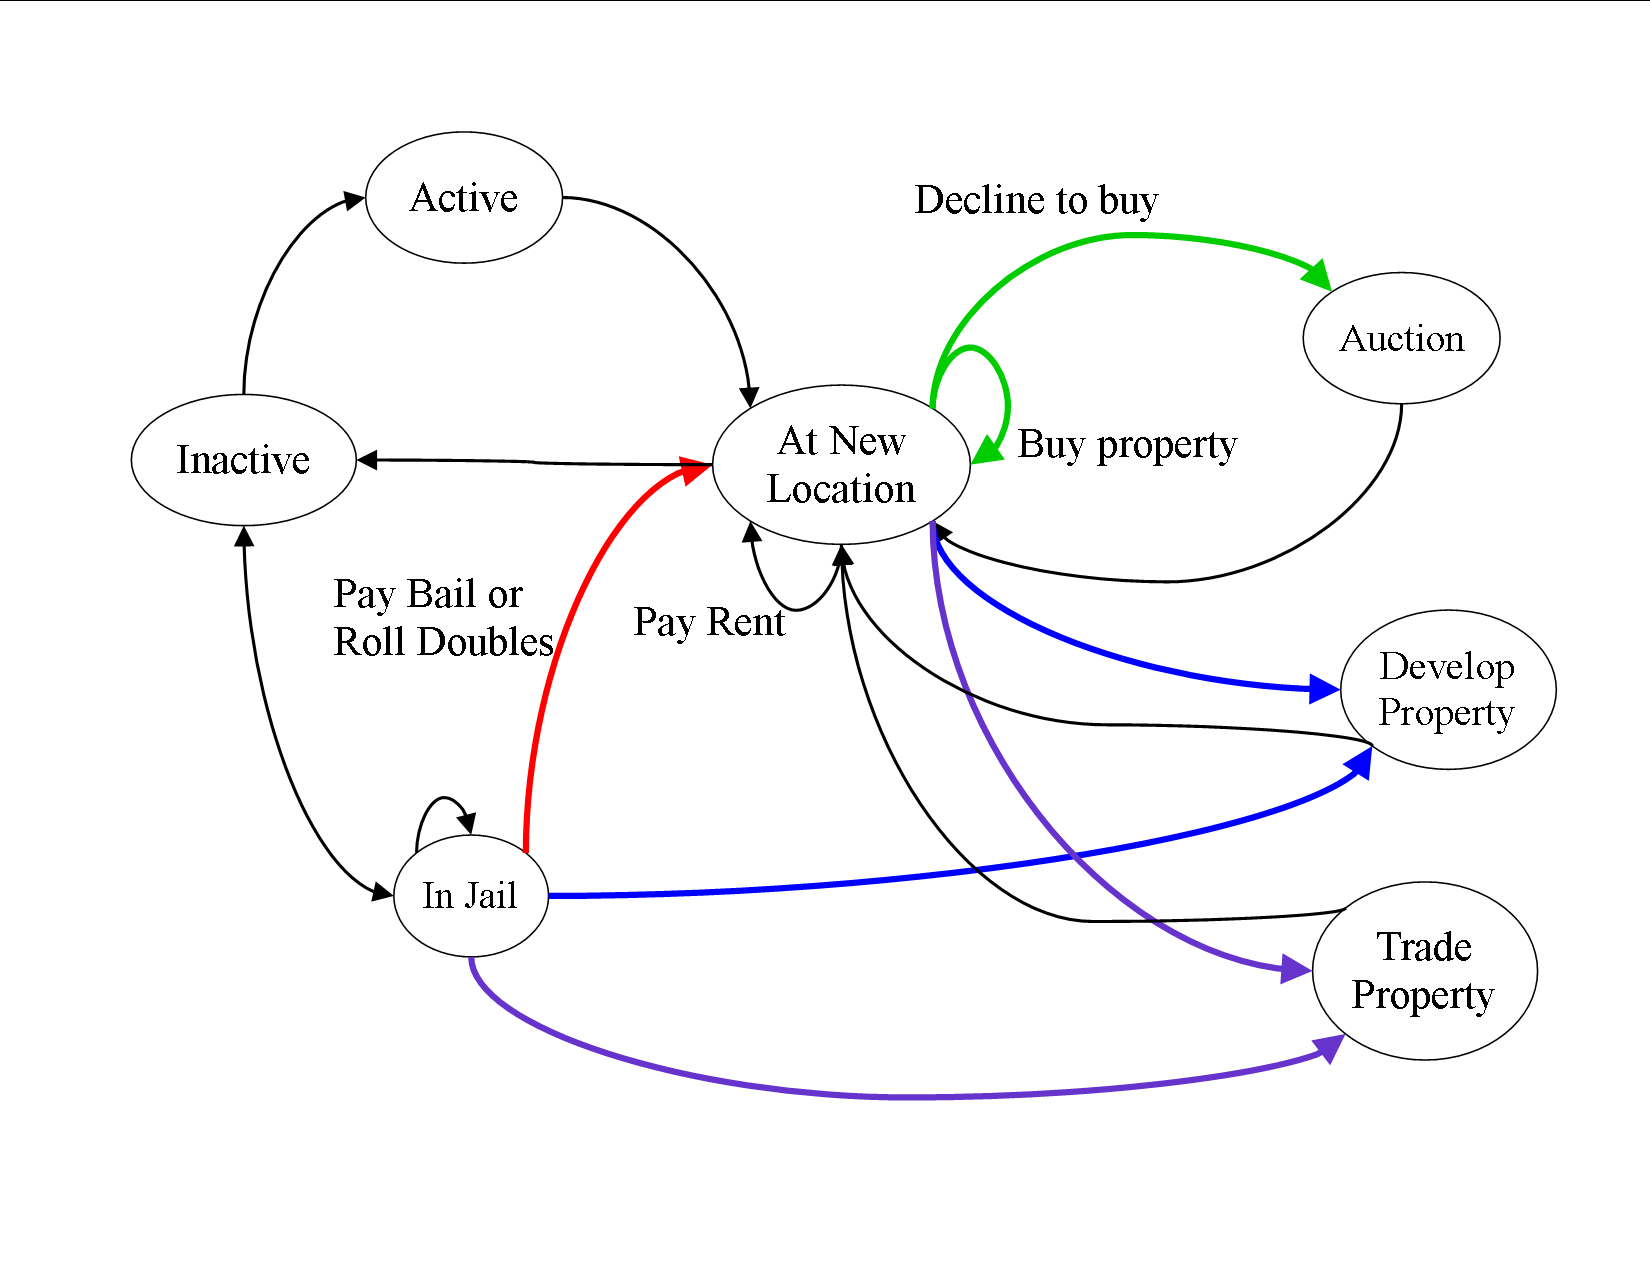
\includegraphics[width=1.0\columnwidth]{Figures/statemachine.png}}
\caption[Monopoly player state machine]{A simplified illustration of the state
machine for a prototype player. Not all state transitions are shown here; for
example, a player can participate in an auction from the inactive state.}
\label{figure-statemachine}
\end{figure}

The decisions that a player makes are whether to buy a property or not (the
arrows numbered 1 in Figure~\ref{figure-statemachine}), whether to pay bail to
exit jail or not (the arrows numbered 2 in Figure~\ref{figure-statemachine}),
whether to buy houses for a property or not (the arrows numbered 3 in
Figure~\ref{figure-statemachine}), and whether to trade a property or not (the
arrow numbered 4 in Figure~\ref{figure-statemachine}).

\subsection{Buying Property}
The primary objective of the game is to acquire and develop properties, and to
obtain monopolies of property groups. When a player lands on an unowned
location, the player must decide whether or not to buy the property. If the
player declines to buy the property, any player, including the player who
declined to buy the property originally, can bid for the property in an auction.
The player must then decide whether to participate in the auction and how much
to bid for the property.

Decisions on whether to buy a property depend on what other properties have been
acquired and which players have acquired them.
  
\subsection{Paying Bail}
When a player is in jail, the player must decide whether to pay bail and exit
jail immediately, or roll the dice and wait until doubles are rolled.

The decision of whether to stay in jail or leave jail depends on what other
properties have been acquired and which players have acquired them.

\subsection{Buying Houses or Hotels}
When a player has a monopoly, the player must decide when and how to buy houses
or hotels for their properties. There are a limited number of buildings in the
game. Whether a player can build depends on what other players have built, and
vice versa.

\subsection{Trading Properties}
The ability to develop a property group depends on the ability of the player to
acquire all the properties in a group. This is done by trading with other
players. When some other player owns one or more properties needed to complete a
monopoly, the player must decide if and when to trade for properties to complete
a monopoly.

\subsection{General Approach}

The four decision areas above led to a preliminary decision to use a multiple
chromosome strategy where different chromosomes will control the player behavior
depending on the state of the game: one strategy for early in the game when few
properties are owned; a different strategy for later in the game when many
properties are owned. Frayn used a similar strategy, except in his study
chromosomes represented the valuation of properties, which depended on ownership
and development factors~\cite{DBLP:conf/cig/Frayn05}.

Additionally, this study used genetic algorithms for just two decisions the
player would make: the buy property decision and the get out of jail decision.
The other two decisions, whether to build a house and whether to trade a
property, were not implemented using genetic computation. The house buying
decision was implemented as a rule based algorithm and is discussed further in
section~\ref{5_buy_house}. The property trading decision was implemented by
adapting a property evaluation function proposed by Yasumura, Oguchi, and
Nitta~\cite{Yasumura2001Negotiate}. We discuss the property trading decision in
Section~\ref{5_trade_property}.

\section{Chromosome description} \label{5_chromo}

The genome for the evolved player consists of multiple chromosomes, each
chromosome used for a different purpose or state of the game. This is in
contrast to the classic simple GA (SGA) where each member of the population has
a single chromosome that is expressed as a string of binary
digits~\cite{haupt2004practical}. Following the initial description of the
genome used in this study, two alternate versions of the chromosome will be
described.

\subsection{Chromosomes for Buying Property}

The first set of chromosomes consists of 4 arrays of real numbers, 40 elements
per array (See Table \ref{table-chromo}). In this thesis, this chromosome is
referred to as the RGA Player (RGA for Real-valued Genetic Algorithm). Each
element of the array represents the probability that the player will purchase
the property represented by the array element. There are 40 locations on the
Monopoly board, so each location corresponds to an element in the array. The
``Go'' space is element 0, with subsequent locations assigned successive element
indices. However, only 28 locations can be owned by a player, so 12 of the array
elements are ignored.\footnote{The chromosome could have been designed with
only 28 locations, but by using 40 elements, the need to create a mapping
between locations and array elements is avoided (improved code readability and
maintainability) at a small cost of memory for the 12 unused elements.}

Each array corresponds to one of the following game states:

\begin{enumerate}
  \item{The first array is used when no player owns any property in the group
  where the player is currently located.}
  \item{The second array is used when the current player owns at least one
  property in the group where the player is currently located and no other
  player owns property in that group.}
  \item{The third array is used when one other player owns property in the
  property group where the player is currently located.}
  \item{The fourth array is used when two other players both own property in the
  property group where the player is currently located.}
\end{enumerate}

\begin{table}[ht]
\caption{Chromosome Illustration}
\begin{center}
\begin{tabular}{|l|c|c|c|c|c|}
\hline
\multicolumn{1}{|l|}{\backslashbox{Location}{Chromosome}}
& \multicolumn{1}{|c|}{Chr1}
& \multicolumn{1}{|c|}{Chr2}
& \multicolumn{1}{|c|}{Chr3}
& \multicolumn{1}{|c|}{Chr4} 
& \multicolumn{1}{|c|}{Etc\ldots } \\ \hline
0 - Go &  ignored  &  ignored &  ignored & ignored & \ldots \\ \hline 
1 - Mediterranean Ave &  $0.615$  &  $0.540$  &  $0.611$ & $0.654$ & \ldots \\ \hline 
2 - Community Chest &  ignored  &  ignored &  ignored & ignored & \ldots \\ \hline 
3 - Baltic Ave &  $0.288$  &  $0.532$  &  $0.165$ & $0.088$ & \ldots \\ \hline
4 - Income Tax &  ignored  &  ignored &  ignored & ignored & \ldots \\ \hline
5 - Reading Railroad & $0.129$  &  $0.649$  &  $0.965$ & $0.390$ & \ldots \\ \hline 
6 - Oriental Ave & $0.834$  &  $0.310$  &  $0.593$ & $0.738$ & \ldots \\ \hline
Etc\ldots & \ldots & \ldots & \ldots & \ldots & \ldots \\ \hline
\end{tabular}
\label{table-chromo}
\end{center}
\end{table}

Each gene in the chromosome represents the probability that the player will make
a positive decision. That is, when the player lands on an unowned street
location, the player must decide whether or not to buy the street. A random
number is generated, and if that random number is less than the gene value, the
player has ``decided'' to buy that street.

Based on the game strategies listed earlier (Section \ref{m_gamestrategies})
we expect that the 4th chromosome will tend to have values that are generally
less than the values in the 1st, 2nd and 3rd chromosomes. That is, the player
will tend to decide to buy property more often when no other player owns any
properties in the group (1st chromosome), and when the property is needed to
complete a monopoly (2nd chromosome), and when the property is needed to block
another player (3rd chromosome).

\subsection{Chromosomes for Paying Bail}

The other set of chromosomes is used to determine when to pay to get out of
jail, and when to remain in jail (and hopefully not roll doubles with the dice).
This chromosome is a 2-D array of real numbers.

Rows and columns in the array are indexed by 6-bit numbers created by the
properties on one side of the board. The first index corresponds to the west
side of the board; the second index corresponds to the north side of the board.
These are the sides of the board on which the player is most likely to land
immediately after leaving jail. For each property on the west or north side of
the board, the corresponding bit in the index is set to 1 if the property is
owned by some other player; otherwise, it is set to 0. For example, there are
six properties on the west side of the board. In board order they are St Charles
Place, Virginia Ave, States Ave, St James Place, New York Ave, and Tennessee
Ave. If opponents owned the first three, then the index would be $000111_2$. The
second index is formed similarly. The two indices are then used to access an
element in the array.

The value at the element is a real number which represents the probability that the
player will choose to pay the bail. When the player is in jail, if a randomly
generated number is less than the gene value, the player has ``decided" to pay
bail. Note that this scheme automatically accounts for different game states:
early in the game very few of the properties are owned (none when the game
begins) so the indices will be near (0, 0); later in the game, if many
properties are owned by other players, the indices will be near (63, 63). It
also accounts for differences in ownership. That is, if opponents own many
properties on the West and North edges, the indices will be relatively high,
whereas if the player owns many of the properties, the indices will be
relatively low. So, if the player owns properties near the jail, his jail
decision will be similar to the decision made early in the game when few
properties are owned.

\subsection{Alternate Chromosome for Paying Bail} \label{5_altjail}

Because the 64x64 array described above consumes a relatively large amount of
memory, this study also looked at an alternate genome which varied this
chromosome by making it a 4x4 array. Instead of indexing by which players owned
properties on the west and north edges of the board, the indices were created by
determining if any of the four color groups on the west and north edges are part
of a monopoly owned by an opponent. This only requires a two-bit index and 16
array elements. The players that use this alternate Jail chromosome will be
referred to as the TGA Players\footnote{Unlike the R (for Real) in RGA, or the S
(for Simple) in SGA, the T in TGA has no meaning. It was chosen because it
follows R and S alphabetically.}.

\subsection{Alternate Chromosome description} \label{5_altchromo}

Goldberg described the chromosome structure of the SGA in \emph{Genetic
Algorithms in Search, Optimization, and Machine
Learning}~\cite{goldberg1989genetic}. The SGA uses a single string of
binary bits for its chromosome. Although the primary population used in this thesis
consists of real valued chromosomes described above, the same information could
be encoded into a binary strings.

Start by representing a decision as a 6-bit gene. If each gene is interpreted as
an integer, then each gene will have some value from 0 to 63. Each value is also
interpreted as the chance of making a positive decision. Just as with the RGA
chromosome, when a decision is required, a random integer between 0 and 63
inclusive is generated; if that random value is less than the chromosome value,
then the player has ``decided'' to buy the property. Thus, each gene has a
coarseness of approximately 1.56\% for each decision.

We then take all the genes and concatenate them into a single string. So, for
example, the first chromosome of 40 elements in the RGA becomes a single string
of 240 bits (6 bits * 40 elements). Each of the other property buying
chromosomes is encoded in the same way.

Likewise, the 4x4 chromosome for paying bail is then encoded as a 96 bit string
(16 genes x 6 bits per gene). This chromosome uses the simplified indexing
scheme described previously in section~\ref{5_altjail}.

A population of these individuals, referred to as Simple GA (SGA) Players, was
also simulated in this study.

\section{House buying algorithm} \label{5_buy_house}

The decision of when to buy houses or hotels was implemented using a simple rule
based procedure. The procedure is summarized in Algorithm~\ref{alg_buyHouse}. 

\begin{algorithm}
\caption{House Buying Algorithm}
\label{alg_buyHouse}
\begin{algorithmic}
\IF{not player has monopoly} 
  \STATE exit
\ENDIF

\IF{not player has sufficient cash} 
  \STATE exit
\ENDIF

\WHILE{player has sufficient cash}
  \IF{player has less than 3 houses on all monopolies}
    \STATE buy house for a property with less than 3 houses
  \ELSE
    \STATE buy 4th house or a hotel for a property
  \ENDIF
\ENDWHILE
\end{algorithmic}
\end{algorithm}

The algorithm begins by checking that the player has a monopoly. If the player
does not have a monopoly, the algorithm exits since the player cannot buy
houses.

Then the algorithm checks that the player has enough cash. We followed Frayn's
procedure for computing the minimum cash a player should keep
available~\cite{DBLP:conf/cig/Frayn05}. The minimum cash a player should keep
available is 200 plus 1\% of the total net worth of all players in the game plus
1\% of the average net worth of the players in the game plus 10\% of the cost of
all houses and hotels currently on the board.
\begin{equation*}
200 + 0.01 \cdot totalNetWorth + 0.01 \cdot avgNetWorth + 0.1 \cdot costOfHouses
\end{equation*}
For the player to have enough cash to buy a house or a hotel, the player must
have the minimum cash plus enough to buy a house or hotel for whichever
monopolies the player owns. If the player does not have enough cash, the
algorithm exits.

If the player has enough cash, then the player buys houses for all monopolies
that have less than 3 houses on them\footnote{The greatest return for a player
occurs when building 3 houses on all properties, and not building 4 houses or a
hotel until all monopolies have 3 houses~\cite{orbanes2007monopoly}.}. If the
player has more than one monopoly, houses are bought for groups in this order:
Orange, Light Blue, Red, Purple, Dark Blue, Yellow, Green, Brown. This order was
chosen based on previous statistical analysis of the value of various property
groups~\cite{Ash1972,Abbott1997,DBLP:conf/cig/Frayn05}. If all monopolies owned
by a player have at least 3 houses on all propeerties, the algorithm will buy a
4th house, and then a hotel for the properties owned by the player.

\section{Property Trading Algorithm} \label{5_trade_property}

For the evolutionary phase of this research, the genetic algorithm players
played without the ability to trade properties. This allowed the players to
evolve strategies for buying properties independent of the option for trading
properties. With the ability to trade, players could learn to forego better
properties in the expectation that the property could be acquired later through
a trade. Also, players might learn to buy less valuable properties at a higher
rate than expected so that the properties could be traded.

However, when it came time to play-test the GA players against human players, a
trading algorithm was needed so that human players would not be bored by a game
that was simply about which player was luckiest in landing on valuable
properties, or which player was lucky enough to acquire a monopoly by chance.

A trading algorithm was implemented based on research by Yasumura, et
al,~\cite{Yasumura2001Negotiate} as the basis for property trading by the A.I.
players in the human-A.I. competition. The human players were, of course, free
to use their own criteria for evaluating whether or not to trade properties. As
we briefly discussed in Section~\ref{3_trading}, Yasumura, et al, developed an
evaluation function that was the sum of some combination of expected gains
(Algorithms~\ref{alg_stg}, \ref{alg_mtg}, and \ref{alg_ltg}) minus expected
losses (Algorithms~\ref{alg_stl} and \ref{alg_mtl}); which gains and losses
are included in the summation is based on the ownership situation of the
properties (See Algorithm~\ref{alg_bigU}. The player's decision would be based
on the result of the evaluation function and whether the player was weighted more towards avoiding losses or
seeking gains.

Expected short term gain \(E_S\) for player \(s\) getting a property card in a
trade is the sum of the probabilities that another player \(i\) will land on the
traded property or one of the properties in the same group in one dice throw
(\(P_S(i)\)) multiplied by the rental fee of the color group (\(R(M)\)) if the
owner used all their available cash \(M\) to buy houses for the color group.
\begin{algorithm} 
\caption{Compute Short Term Gain}
\label{alg_stg}
\begin{algorithmic}
   \STATE $E_S \gets \sum P_S(i) \cdot R(M)$ 
\end{algorithmic}
\end{algorithm}

Expected mid term gain \(E_M\) is the sum of the probabilities that another
player will land on the traded property or one of the properties in the same group in
one trip around the board multiplied by the rental fee of the color group if the
owner were used all their available cash to buy houses for the color group.
\begin{algorithm} 
\caption{Compute Mid Term Gain}
\label{alg_mtg}
\begin{algorithmic}
   \STATE $E_M \gets \sum P_M(i) \cdot R(M)$ 
\end{algorithmic}
\end{algorithm}

Expected long term gain \(E_L\) is the sum of the probabilities that another
player will land on the traded property or one of the properties in the same group in
one trip around the board multiplied by the rental fee of the color group if the
owner had \$1000 to buy houses for the color group.
\begin{algorithm} 
\caption{Compute Long Term Gain}
\label{alg_ltg}
\begin{algorithmic}
   \STATE $E_L \gets \sum P_M(i) \cdot R(1000)$ 
\end{algorithmic}
\end{algorithm}

The short term loss is simply the probability that the player \(s\) making the
trade will land on the property being traded on the next dice roll, multiplied by the
rent for that property if the new owner used all their cash to buy houses for
that property.
\begin{algorithm} 
\caption{Compute Short Term Loss}
\label{alg_stl}
\begin{algorithmic}
   \STATE $L_S \gets P_S(s) \cdot R(M)$ 
\end{algorithmic}
\end{algorithm}

The potential mid-term loss is the probability that the player \(s\) making the
trade will land on the location in one trip around the board multiplied by the rent
for that property.
\begin{algorithm} 
\caption{Compute Mid Term Loss}
\label{alg_mtl}
\begin{algorithmic}
   \STATE $L_M \gets P_M(s) \cdot R(M)$ 
\end{algorithmic}
\end{algorithm}

Finally, the various expected gains and losses are summed based on the property
ownership situation. There are 4 cases to evaluate: 1) the player \(s\) would
receive one card \(c\) of a given color group; 2) the player would have two
cards in a color group and one would be in the bank; 3) the player would have two cards in
a color group, and another player would have the remaining card(s); or 4) the
player would have a monopoly after the trade.
\begin{algorithm} 
\caption{Evaluate Property}
\label{alg_bigU}
\begin{algorithmic}
  \IF {Case~1}
    \STATE $f(c) \gets \phi(c) \gets 1/2 \cdot FV(c) + E_L(c)$
    \COMMENT FV(c) is the face value, or cost, of the property card \(c\)
  \ENDIF
  \IF {Case~2}
    \STATE $f(c) \gets 2 \cdot \phi(c) + E_M(c)$
  \ENDIF
  \IF {Case~3}
    \STATE $f(c) \gets 2 \cdot \phi(c) + E_M(c) + E_S(c)$
  \ENDIF
  \IF {Case~4}
    \STATE $f(c) \gets 3 \cdot \phi(c) + \alpha \cdot (E_M(c) + E_S(c))$
  \ENDIF

  \REQUIRE $\omega_1 + \omega_2 = 1$

  $U \gets \omega_1(\sum f(c) + M) - \omega_2(L_S + L_M)$
\end{algorithmic}
\end{algorithm}

After summing the gains, and weighting the sum by \(\omega_1\), the function
subtracts a weighted sum of the short-term and mid-term losses. The factor
\(\omega_1\) biases the function towards gain seeking; a high \(\omega_1\) means
the player will favor gains over avoiding losses. The factor \(\omega_2\) biases
the function towards avoiding losses; when \(\omega_2\) is high the player will
avoid trades that lead to potential losses. If the value of the function, \(U\)
exceeds a given threshold, the player will propose the trade, or accept a
proposed trade. 

Yasumura, et al, evaluated 5 thresholds from a low value of 100
to a high value of 500. They found the best profits were generated by agents
that used the lowest threshold, so the the algorithm used in the human versus
computer competitions used a threshold of 100 also. However, it appears that
this threshold may have led to poor performance of the RGA players during the
human versus computer competition. This is discussed in detail in Section 6.x.

\section{Fitness Evaluation} \label{5_fitnesseval}

Six different fitness evaluations were used for the genetic algorithm. Three of
the fitness evaluations are based on which player wins a game, and in which
order the other players finish. The winner of each game is the last player left
in the game, or the player with the greatest net worth when the game finishes.
The second place player is the second to last player in the game, or the player
with the second greatest net worth when the game finishes. Third and fourth
place players are determined similarly. The different evaluators award fitness
points to the players as follows.

\begin{enumerate}
  \item {Finish Order (FINISH\_ORDER); in a game with \(n\) players, the winner
  of the game receives \(n-1\) points; second place receives \(n-2\) points, and
  so on. The last place finisher receives 0 points.}
  \item {Number of wins (NUM\_WINS); the winner of each game receives three
  points; all other players receive zero points.}
  \item {Number of Properties owned (NUM\_PROPERTIES); each player receives one
  point per property owned at the end of the game.}
  \item {Number of Monopolies (NUM\_MONOPOLIES); each player receives one
  point for each monopoly they control.}
  \item {Net Worth (NET\_WORTH); at the end of each game, the net worth of each
  player is calculated. Each player receives points that equal their net
  worth.}
  \item {Tournament level (TOURNAMENT); players compete in a modified single
  elimination tournament. The fitness score is the level attained in the
  tournament tree.}
\end{enumerate}

The first two fitness evaluators that were developed followed directly from
the work of Frayn, and indirectly from previous studies of genetic
algorithms and games. Frayn competed chromosomes against each other in
four-player games. The winner of each game received +3 points, the second place
finisher received +2, etc. This is very similar to the competitions discussed in
Chapter~\ref{chap:background}, where the winner in two-player games such as
Tic-Tac-Toe, Checkers, and Othello received points for winning a game, and the
loser received 0 points. Since Frayn used four players in each game, second and
third place finishers also receive some points (although less than the winner);
the last place finisher still gets 0 points. This fitness evaluator is named
FINISH\_ORDER and uses the same 3/2/1/0 point scale to award scores in a game.
We also use a simplified 3/0/0/0 fitness measurement named NUM\_WINS where the
winner receives +3 and every other player receives 0.

We also reason that players who win the game of Monopoly tend to acquire more
properties and more monopolies of properties. So two more fitness functions were
developed. One labeled NUM\_PROPERTIES that counts the number of properties that
a player owns and awards +1 point for each property. The other fitness function
is labeled NUM\_MONOPOLIES and it awards +1 points for each monopoly controlled
by a player.

Then there is a fitness function named NET\_WORTH. For each game played in the
simulation, the winner is the last one left in the game or the player with the
highest net worth (cash plus value of properties) in the game if not all players
go bankrupt. Thus the winner of the game will always have the highest net worth.
For each player in a game, NET\_WORTH computes the ratio of each player's net
worth to the total net worth of a game (the sum of the net worth of all the
players in the game). The ratio is then multiplied by 100 and the value is
awarded to the player as their score for the game.
\begin{equation*}
score = 100 * net\_worth / total\_net\_worth
\end{equation*}
Last is the TOURNAMENT fitness evaluator (discussed in more detail
in~\ref{5_compfit}. A modified single elimination tournament is conducted in
each generation. The fitness score of each player is the level the player
attains in the tournament tree, starting at level 0. So, the losers of the first
round get a score of 0, and the winners get +1. This continues until only two
players remain.

After all the games in a generation have been played, the scores are normalized
to a 100 point scale (except for TOURNAMENT). For the first four fitness
evaluators, this is a simple calculation for each player \(i\).
\begin{equation*}
score_{normalized} = 100 * (score_i - min(score)) / (max(score) - min(score))
\end{equation*}
The minimum score (\(min(score)\)) for every generation is simply 0. The maximum
score (\(max(score)\)) is the maximum score for any single game (i.e. 3 for NUM\_WINS
and FINISH\_ORDER, 28 for NUM\_PROPERTIES, and 8 for NUM\_MONOPOLIES) multiplied
by the number of games that each player competes in (See~\ref{5_evoprop}). 

For the NET\_WORTH evaluator, the process is a little more involved. While the
minimum score is still 0, the maximum score in a generation is not fixed. The
evaluator must keep track of the maximum score for a generation, and then use
that at the end of the generation to normalize the scores. Otherwise, the
calculation is the same.

The NUM\_WINS, FINISH\_ORDER, and NET\_WORTH evaluators are the evaluators that
are direct competitive fitness functions. When using those evaluators, the
fitness of the players is based directly upon their performance against other
players. 

The other two evaluators are only indirectly competitive. When players compete
against each other in the game, we expect that the winner of the game will
acquire more properties or will acquire more monopolies than the other players.
So on average, the winning player of a game will have more properties or more
monopolies than the losing players. However, that is not necessarily the case.
as mentioned above, the winner of a game can be the player with the greatest net
worth. With NUM\_PROPERTIES and NUM\_MONOPOLIES, that the player with the
greatest net worth may not have the most properties or the most monopolies.

\section{Evolution and Propagation} \label{5_evoprop}

The parameters used in the genetic algorithm are based on the parameters used by
Frayn, with some modifications based on other research into coevolution,
competitive fitness functions, and games. We start by looking at how Frayn ran
his population evolution, and then follow with an explanation of the parameters
used in this project.

\subsection{Frayn's evolutionary parameters}

Table~\ref{table-fraynparams} shows the parameters that Frayn used when creating
and evolving the population of game players in his
research~\cite{DBLP:conf/cig/Frayn05}. His research used a competition method
similar to K-Random Opponents with \(K=300\), and a population size of 1000. As
mentioned previously, he used a single fitness measurement that awards points
based on the place-finish of each player in the game.

\begin{table}[ht]
\caption{Frayn's Evolution Parameters}
\begin{center}
\begin{tabular}{ | l | l | }
  \hline                        
  Population size: & 1000 \\ \hline
  Matches per generation: & 100 \\ \hline
  Number of players per game: & 4 \\ \hline
  Games per match: & 250 (1000 players/4 players per game) \\ \hline
  Fitness: & Game winner	+3 \\
  & Game 2nd place	+2 \\
  & Game 3rd place	+1 \\
  & Game 4th place	+0 \\
  & (Max score per generation is 300) \\ \hline
  Reproduction: & Elitism and reproduction, with crossover and mutation \\ \hline  
\end{tabular}
\label{table-fraynparams}
\end{center}
\end{table}

Frayn's process was as follows. 

\begin{enumerate}
  \item Initialize a population of 1000 individuals.
  \item Each individual plays 100 games.
  
  \begin {itemize}
    \item The 1000  individuals are randomly divided into 250 sets of 4.
    \item These 250 sets each play a game. Points are awarded at the end of the
    game.
    \item After all 250 games are complete, the 1000 individuals are again
    randomly divided into 250 different sets, and the sets play again.
    \item Repeat until each individual has played 100 games.
  \end{itemize}
  
  \item At the end of the generation, the total number of points earned by each
  individual is evaluated as the fitness of the individual.
  \item The new population of 1000 players is created.
  \begin{itemize}
    \item Top 3 players move into next generation (elitism).
    \item 300 players chosen by tournament selection with replacement.
    \item 300 players chosen by tournament selection with replacement and then
    mutated.
    \item 397 children created by selecting parents using tournament selection
    with replacement, and then applying uniform crossover to the parents'
    chromosomes.
  \end {itemize}
\end{enumerate}

Note that each player in a generation plays 100 games against 300 other
opponents (3 different opponents for each game). So the competitive fitness
function used by Frayn is K-Random Opponents with \(K\approx300\). K is
approximate because the three opponents are selected independently for each
game, so it is possible for the same opponent to be selected in more than one
game. Over the total span of his study, Frayn reported that his project
included over 377 million simulated games.

\subsection{Evolutionary parameters used in this research}

The last remaining task is to decide on the parameters to be used for the
genetic algorithm. The success of any genetic algorithm is highly dependent on
the parameters chosen. Parameters will be chosen using guidance from previous
studies. The thought is that if those parameters worked for previous studies
they will likewise lead to successful solutions in this study.

\subsubsection{Population size}

Chapter~\ref{chap:background} summarized several research studies that used
genetic algorithms to develop game players. When Fogel evolved neural networks
to play Tic-Tac-Toe, his population consisted of 50
individuals~\cite{Fogel1993}. The population for Checkers was 30
individuals~\cite{Fogel2000Anaconda,journals/tec/ChellapillaF01}.
The population for Othello was 20 individuals~\cite{ChongTW05}. When
Ja\'{s}kowski et al., introduced Fitnessless Coevolution, they used population
sizes comparable to those used in previous research that used the same
optimization problems~\cite{Jaskowski:2008:FC:1389095.1389161}.

In this research, we follow Frayn's lead by starting with a population size of
1000. However, to implement a modified single elimination tournament competition
it will be necessary to modify this value slightly to be 1024. In addition,
based on the results of some of the comparative studies of competitive fitness
functions~\cite{Angeline:1993:CEE:645513.657590, Panait02acomparative,
Jaskowski:2008:FC:1389095.1389161}, we also investigate the behavior of smaller
population sizes such as 32, 128, and 512. The value 32 is chosen because it is
similar to the population sizes of those other studies; the other two sizes of
128 and 512 were chosen to provide intermediate population sizes between 32 and
1024.

We feel comfortable with an initial assumption that valid results might be
obtained with a population size as small as 32. Chapter~\ref{chap:background}
listed the state space complexity of various games to which genetic algorithms
had been applied. If the state space complexity of Monopoly is comparable to
those games, then the use of a small population size is a reasonable initial
assumption.

Note that there are 28 locations on the Monopoly board that can be owned by a
player. Any location can be unowned, or can be owned by one of the four players.
This gives an initial state space estimate of \(5^{28}\), or approximately
\(10^{19.6}\). This is within two orders of magnitude of Checkers at
\(\approx10^{18}\). 

Now consider that houses can be built by a player on a property. Since houses
can only be built when one player owns all street locations in a property group,
only some state space configurations will allow houses or hotels. Assume
\(Player_{i}\) has a monopoly in the first or last color group on the board
(where there are two locations that can be built upon) and there are no other
monopolies. Then the number of additional state space configurations for either
group is
\begin{equation*}
4 \cdot 10 \cdot 5^{26} \approx 10^{19.8}
\end{equation*}
where 4 is the number of players that could have the monopoly, 10 is the number
of houses (2 streets with up to 4 houses or 1 hotel each), and \(5^{26}\) is the
state space for the remaining 26 locations on the board. If there is a single monopoly
in one of the other color groups (with 3 streets in the group), then the
calculation is
\begin{equation*}
4 \cdot 15 \cdot 5^{25} \approx 10^{19.3}
\end{equation*}
So, considering just properties and single monopolies, the total state space
is
\begin{equation*}
5^{28} + 2 \cdot 4 \cdot 10 \cdot 5^{26} + 6 \cdot 4 \cdot 15 \cdot 5^{25}
\approx 10^{20.4}
\end{equation*}
As we consider multiple monopolies, the size of the state space will continue to
grow, but at a slower rate. This is because the exponential term becomes smaller
(e.g. for two monopolies the exponential term is \(5^{22}\), \(5^{23}\), or
\(5^{24}\) and the total complexity only rises to \(\approx10^{20.5}\)) and
because there is a limit to the number of houses that can be bought. Thus it is
clear the game has a state space complexity less than that of Othello at
\(\approx10^{30}\).

\subsubsection{Competitive fitness} \label{5_compfit}

The populations are tested using both K-Random Opponents and a modified
version of Single Elimination Tournament.

Again following Frayn, each player in the population competes in 100 games per
generation, which equates to approximately 300 opponents\footnote{The number of
opponents is approximate because of the random nature in which matches within a
generation are intialized. After all players play a single game, the players are
all returned to the player pool and are randomly selected again for the next
game. So just by chance alone, some players will play each other more than once
in a generation. For populations with a small size and a large number of games
such as a population of 32 players that plays 100 games per generation, players
will definitely play each other more than once in a single generation. For large
populations that play small numbers of games per generation (e.g. pop. size=1024
and number of games=7) it is less likely to occur.}. However, because Panait
and Luke, and Ja\'{s}kowski et al., had success with smaller values of K for the
optimization problems they studied, this research also looks at K-Random
Opponents where the number of games played by a player is \(K=21\) (7 games),
\(K=75\) (25 games), and \(K=150\) (50 games). After each player completes a
game, a fitness score is computed by one of the fitness evaluators described
earlier. The player's total fitness is the sum of scores after all games in a
generation are complete.

This research will also use a modified version of Single Elimination Tournament
(SET). With two player games, SET pairs the players in a generation, competes
each pair, and eliminates the losers, until a single player is left.
Fitness is the number of games won, or equivalently the level attained in the
tournament tree. Since four players compete in every Monopoly game in this
research, SET is modified by eliminating the bottom two players in each game and
advancing the top two players to the next level. At the final level, the last
two remaining players get the same fitness score.

We set the number of players in a generation to be a multiple of four so that
SET would be easier to implement. Population numbers that are not multiples of
four would require implementing the simulator to give some players
byes\footnote{A bye is when a participant in a tournament automatically
advances to the next level automatically without playing a game at the current
level.} for some matches, and keeping track of that information. It is easier
just to specify that the population size is a multiple of four, so that no byes
are necessary. So that is why Frayn's population of 1000 was changed to 1024 for
this research.

\subsubsection{Reproduction}

After each generation, the current population is propagated into a new
population using reproduction, recombination, and mutation. Again, this study
uses parameters similar to those used by Frayn, but with some modifications.

\begin{itemize}
  \item {The top 10\% of individuals are copied into the new generation
  (elitism).}
  \item {30\% of the new population is created by selecting individuals through
  tournament selection and copying them into the new generation.}
  \item {Another 30\% of the new population is created by selecting individuals
  through tournament selection, mutating them, and then copying them into the new
  generation.}
  \item {The final individuals are created by selecting parents using
  roulette wheel selection, and then combining the chromosomes to create two
  new children. The child chromosomes are created by arithmetic crossover using
  the formulas 
  
  \(child_{1} = \beta * parent_{1} + (1 - \beta ) * parent_{2}\)

  \(child_{2} = (1 - \beta ) * parent_{1} + \beta * parent_{2}\)}
\end{itemize}

The parameters used for the genetic algorithm are summarized in
Table~\ref{table-evoparams}.

\begin{table}[ht]
\caption{Evolution Parameters for this Research}
\begin{center}
\begin{tabular}{ | l | l | }
  \hline                        
  Population size: & 32, 128, 512, 1024 \\ \hline
  Matches per generation: & 7, 25, 50, 100 \\ \hline
  Number of players per game: & 4 \\ \hline
  Games per match: & 8, 32, 128, 256 (num players/4 players per game) \\ \hline
  Fitness: & FINISH\_ORDER \\ 
           & NUM\_WINS \\
           & NUM\_PROPERTIES \\ 
           & NUM\_MONOPOLIES \\
           & NET\_WORTH \\ 
           & TOURNAMENT \\ \hline
  Propagation: & Elitism and reproduction, with crossover and mutation \\ \hline  
\end{tabular}
\label{table-evoparams}
\end{center}
\end{table}

\clearpage
\chapter{Results}\label{chap:results}

\section{Overview}

Over 1 billion games were simulated in the process of evaluating the chromosomes
in this experiment. One thousand generations were evolved for every combination
of chromosome type (RGA, SGA, and TGA), population size (32, 128, 512, and
1024), number of games played by each chromosome per generation (7, 25, 50,
100), and fitness evaluator (FINISH\_ORDER (FO), NET\_WORTH (NetW),
NUM\_MONOPOLIES (NM), NUM\_PROPERTIES (NP), NUM\_WINS (NW), and TOURNAMENT
(TO)\footnote{For the tournament fitness evaluator the number of games was
determined by the population size and was not independent. So for TOURNAMENT,
1000 generations were evolved for every combination of population size and
chromosome type}). In this chapter, those four features are used to identify the
different populations: for example, RGA-512-50-NP refers the to RGA chromosome
population of size 512, where each player played 50 games per generation and the
fitness evaluator was NUM\_PROPERTIES. Results of the evolutionary process are
presented in the first section of this Chapter.

Results for the RGA chromosome are presented first, and in a large amount
detail. We also look briefly at the results for the SGA chromosomes, even though
players with this chromosome tended to evolve poorly. This is most likely due to
the fact that the data structure used for the SGA chromosomes is not well suited
to the problem domain. Finally, results for the TGA chromosomes are very briefly
discussed, but these players were essentially identical to the RGA chromosomes
and so do not provide any additional insight.

After the evolutionary process was complete, the best players from each
generation were competed in various combinations to validate the results. The
validation process is listed below. Because the evolution of SGA and TGA
chromosomes do not provide any useful information, the validation of the evolved
players focuses exclusively on results obtained from the RGA chromosomes.

\begin{enumerate}
  \item {Intra-population validation}
  \begin{enumerate}
    \item {For each RGA population select the best player from generation 250,
    500, 750, and 999}
    \item {Compete the 4 players in 100 games}
    \item {Record the fitness scores for FINISH\_ORDER and NUM\_WINS}
    \item {Repeat 50 times with evolution}
    \item {Use Student's t-test to compare average fitness}
  \end{enumerate}
  \item {Inter-population validation for fitness evaluator}
  \begin{enumerate}
    \item {From generation 999 of a set of populations differing only by
    original fitness evaluator, select the best player under each fitness
    evaluator (results in 6 players)}
    \item {Compete the 6 players in 50 games}
    \item {Record the fitness scores for FINISH\_ORDER}
    \item {Repeat 30 times}
    \item {Use Student's t-test to compare average fitness}
  \end {enumerate}
  \item {Real-world validation 1}
  \begin{enumerate}
    \item {Select the top 4 players from generations 250, 500, 750, and 999 from
    the RGA-1024-100-FO population}
    \item {compete the players randomly against human players}
    \item {Record the fitness scores for FINISH\_ORDER}
    \item {Compare average fitness and average net worth among all players}
  \end {enumerate}
  \item {Real-world validation 2}
  \begin{enumerate}
    \item {Select the top 4 players from generation 999 from the RGA-1024-100-FO
    population}
    \item {Compete the players randomly against human players using an updated
    property trading algorithm}
    \item {Record the fitness scores for FINISH\_ORDER}
    \item {Compare average fitness and average net worth among all players}
  \end {enumerate}
\end{enumerate}

First, an intra-population validation was performed where the best players from
different generations within a population were competed against each other.
For example, using the RGA-1024-100-NetW population (a population of RGA players
of size 1024, evolved using 100 games per generation, with the NET\_WORTH
fitness evaluator) select the best player from generations 250, 500, 750, and
999. Compete those 4 players in a set of 100 games and record the cumulative
fitness using FINISH\_ORDER and NUM\_WINS\footnote{Regardless of the original
fitness evaluator used in evolution, the validation experiments use
FINISH\_ORDER and NUM\_WINS to compare players.}. Repeat this process 50 times
without further evolution of the players. We then analyze the player's
performance over the 50 trials to determine if players in later generations were
better than players in earlier generations.

Second, players were also validated with an inter-population validation. That
is, the best players from different populations were competed against each other
in various combinations. For example, given the various RGA-1024-100
populations, select the best player from each fitness evaluator and from
generation 999. This will result in 6 players which then play 50 games against
the other players; record the cumulative fitness using FINISH\_ORDER. Repeat
this process 30 times without further evolution of the players\footnote{The
results of the first validation were extremely strong, which implied that 50
trials and 100 games per trial was excessive; thus the validation parameters
were relaxed for the second validation.}. We then analyze the player's
performance over the 30 trials to determine if different fitness evaluators were
better than others.

The results from the intra- and inter-population competitions are discussed in
the second section of this Chapter.

In the last section of this Chapter, results from games where RGA players played
against human players are presented. Based on the previous intra- and
inter-population validations performed, we picked 4 players from generations
250, 500, 750, and 999 of a population. These evolved RGA players from
various generations were competed against human players. In general, we found
that though the RGA players competed well against other RGA players, they did
relatively poorly against human players. We believe this is due to the property
trading algorithm that was implemented for this competition.

The property trading algorithm was adjusted and a second competition was
performed. With the adjusted trading algorithm, the AI players performed better.
The results of the second competition are also documented in the final section
of the chapter.

\section{Results of the Evolutionary Process}

In this section we look at the results of the evolutionary process. Looking at
the fitness distributions and the chromosomes at the completion of evolution
will show that the players did learn to buy some properties with greater
probability than others.

\subsection{Results for Initial RGA Generations}

In a competitive fitness evolutionary process, we expect that the players will
be randomly spread in their ability to win games. Some players will win games,
some will lose games, and the average player will win about half the games they
play. The distribution of fitness scores should follow a distribution similar to
the binomial distribution (See Figure~\ref{figure-binomial}).

When the initial populations of players was run through a single generation, the
actual results matched the expected results quite closely.

Figure~\ref{figure-RGA-G000-N100-FO-initial_fitness} shows the fitness
distribution for the first generation of the RGA-1024-100-FO population. The
figure shows a binomial shaped distribution which appears to be centered around
the population average of 150\footnote{Because the FINISH\_ORDER evaluator
assigns 1, 2, and 3 points to the players in a game, for a total of 6 points per
game, the average fitness for any single game is \(6/4\) or 1.5. So for \(n\)
games the average fitness is \(n * 1.5\). For a population that plays 100 games
per generation, the fitness distribution will be centered on the average score
of 150.}.

\begin{figure}
\centering
%%----start of first figure----
\begin{minipage}[t]{0.47\linewidth}
\centering
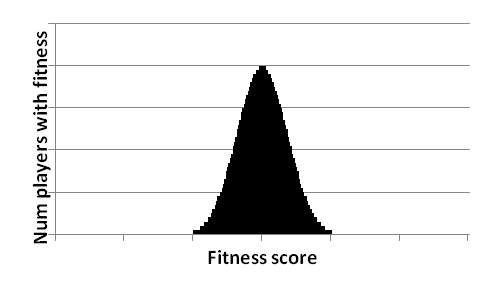
\includegraphics[width=1.0\linewidth]{Figures/binomial.png}
\caption[Binomial Distribution]{The expected fitness distribution for the first
generation of a population that uses a competitive fitness function such as
FINSIH\_ORDER or NUM\_WINS. A peak is expected around the average population
fitness. The distribution is similar to a binomial distribution.}
\label{figure-binomial}
\end{minipage}%
\hspace{0.06\linewidth}%
%%----start of second figure----
\begin{minipage}[t]{0.47\linewidth}
\centering
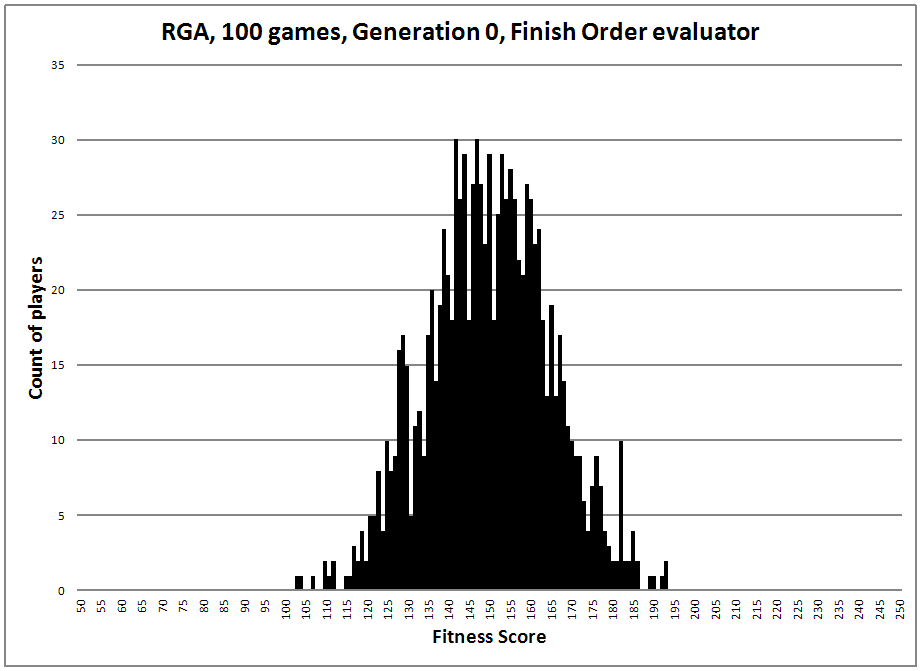
\includegraphics[width=1.0\linewidth]{Figures/RGA_1024_G000_N100_FO.png}
\caption[RGA Finish Order Fitness Distribution, Initial Generation]{RGA
chromosome, size 1024, 100 games per generation, finish order
fitness evaluator, generation 0.}
\label{figure-RGA-G000-N100-FO-initial_fitness}
\end{minipage}
\end{figure}

An example of the fitness distribution for the NUM\_WINS fitness evaluator is
shown in Figure~\ref{figure-RGA-G000-N100-NW-initial_fitness}. The average
fitness for a single game is \(3/4\) or 0.75; for \(n\) games the average
fitness is \(n * 1.5\). The figure shows a binomial shaped distribution which
appears to be centered around the population average of 75.

\begin{figure}
\centering
%%----start of first figure----
\begin{minipage}[t]{0.47\linewidth}
\centering
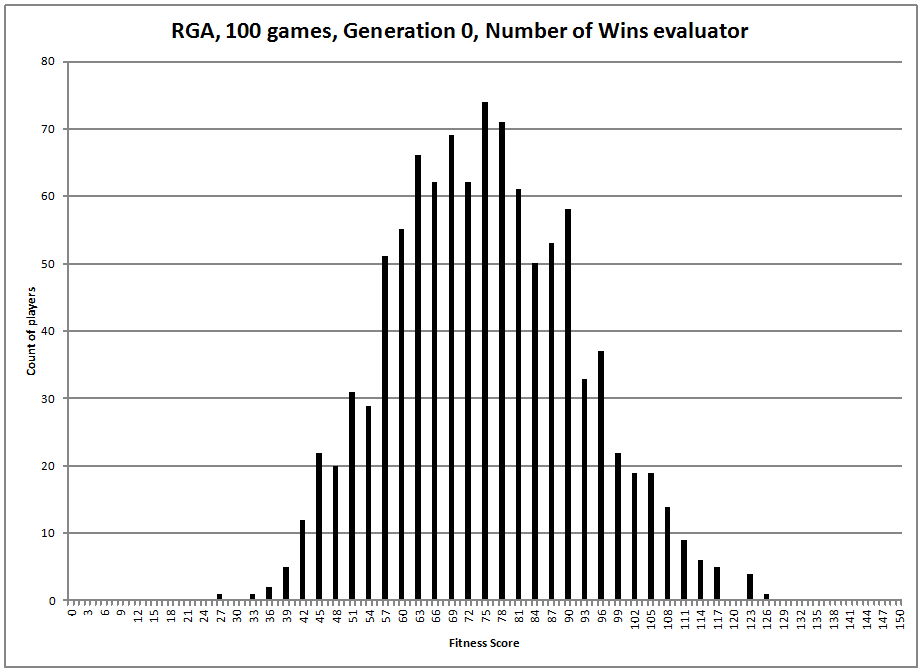
\includegraphics[width=1.0\linewidth]{Figures/RGA_1024_G000_N100_NW.png}
\caption[RGA Num Wins Fitness Distribution, Initial Generation]{RGA chromosome,
size 1024, 100 games per generation, number of wins fitness evaluator,
generation 0.}
\label{figure-RGA-G000-N100-NW-initial_fitness}
\end{minipage}%
\hspace{0.06\linewidth}%
%%----start of second figure----
\begin{minipage}[t]{0.47\linewidth}
\centering
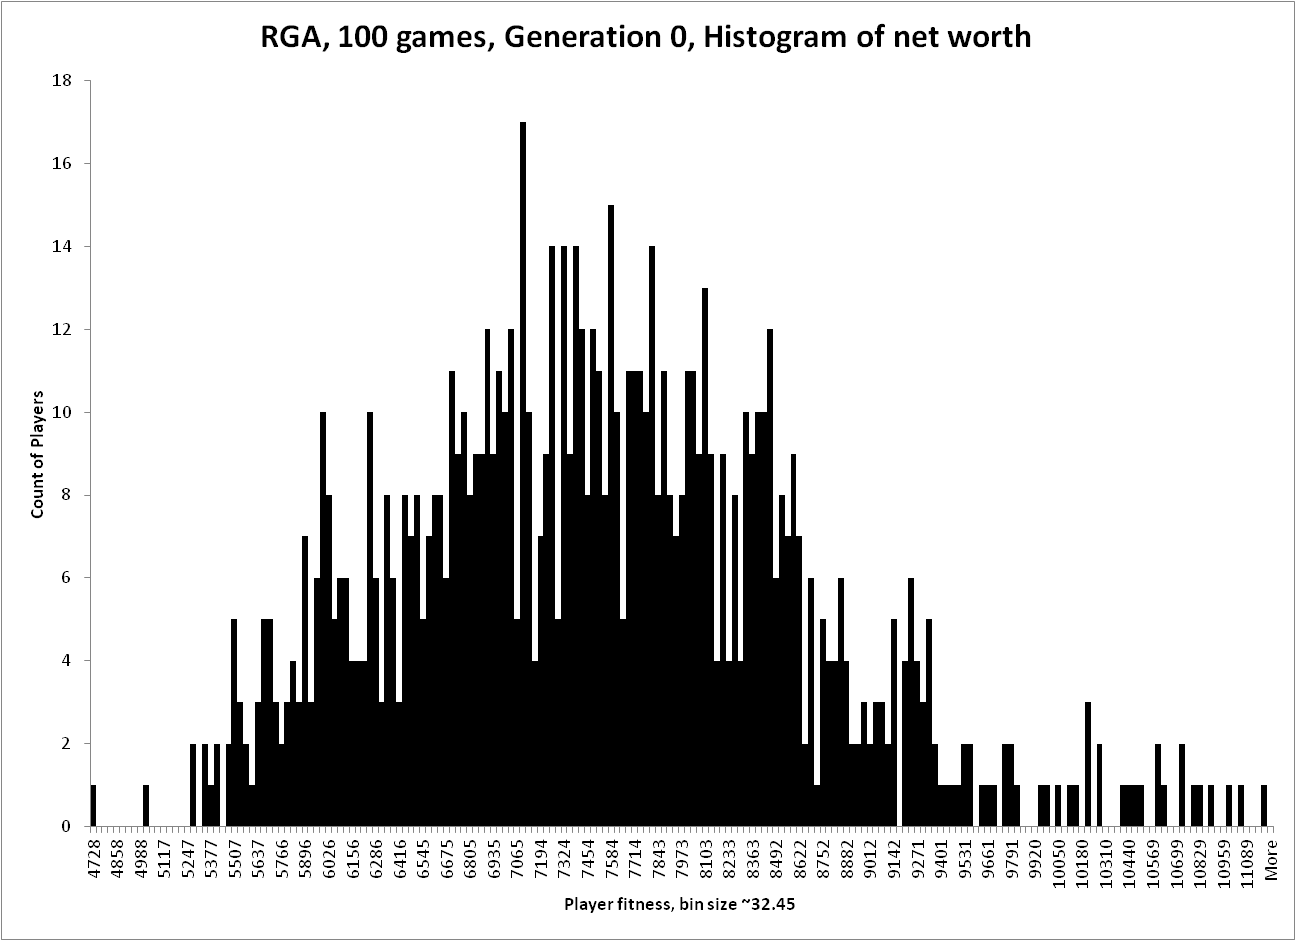
\includegraphics[width=1.0\linewidth]{Figures/RGA_1024_G000_N100_NetW.png}
\caption[Historgram of RGA Net Worth Fitness Distribution, Initial
Generation]{RGA chromosome, size 1024, 100 games per generation, net worth
fitness evaluator, generation 0.}
\label{figure-RGA-G000-N100-NetW-initial_fitness}
\end{minipage}
\\[\intextsep]

\begin{minipage}[t]{0.47\linewidth}
\centering
%%----start of third figure----
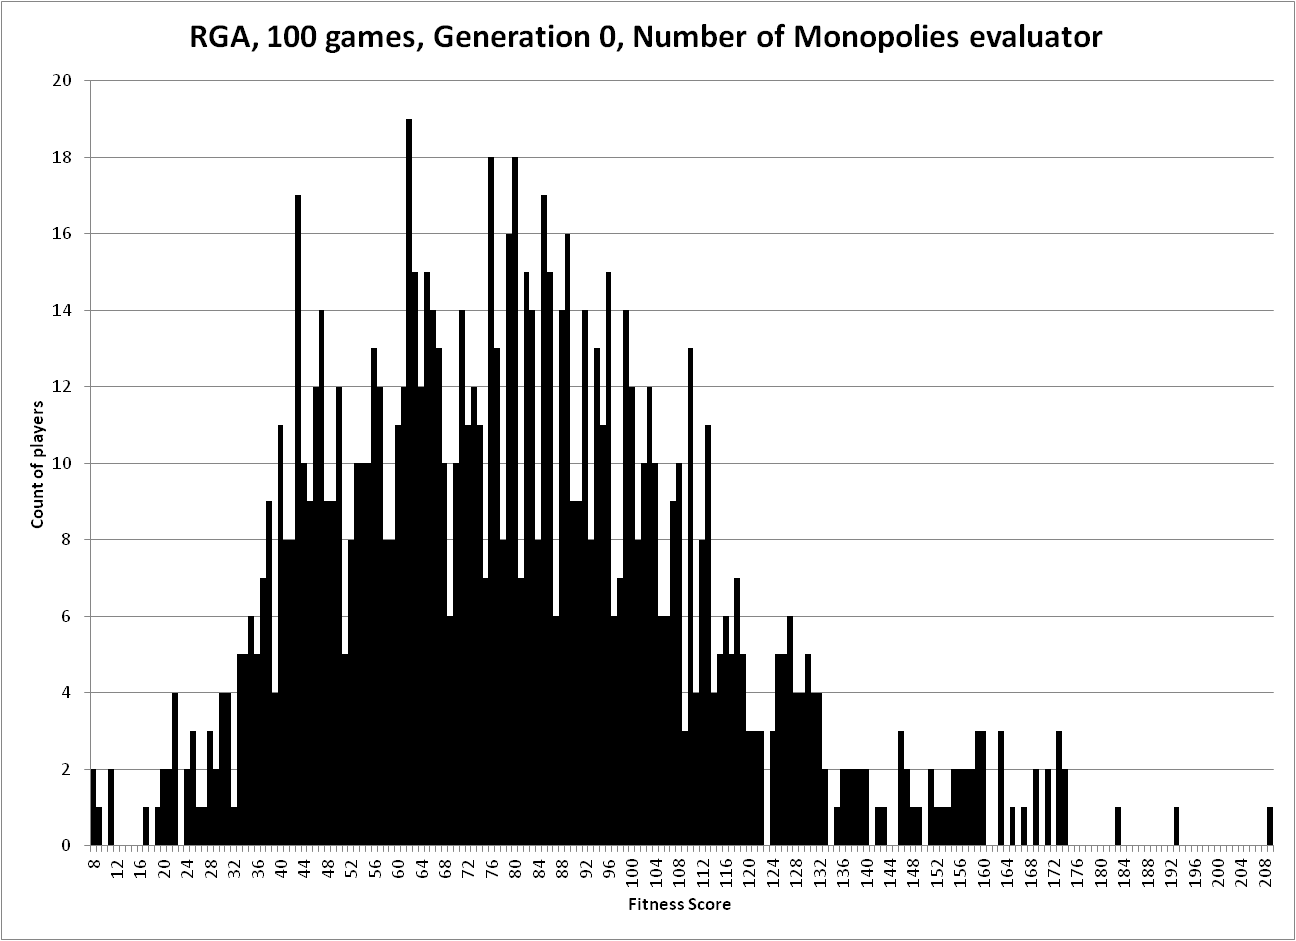
\includegraphics[width=1.0\linewidth]{Figures/RGA_1024_G000_N100_NM.png}
\caption[RGA Num Monopolies Fitness Distribution, Initial Generation]{RGA
chromosome, size 1024, 100 games per generation, number of monopolies
evaluator, generation 0.}
\label{figure-RGA-G000-N100-NM-initial_fitness}
\end{minipage}%
\hspace{0.06\linewidth}%
%%----start of fourth figure----
\begin{minipage}[t]{0.47\linewidth}
\centering
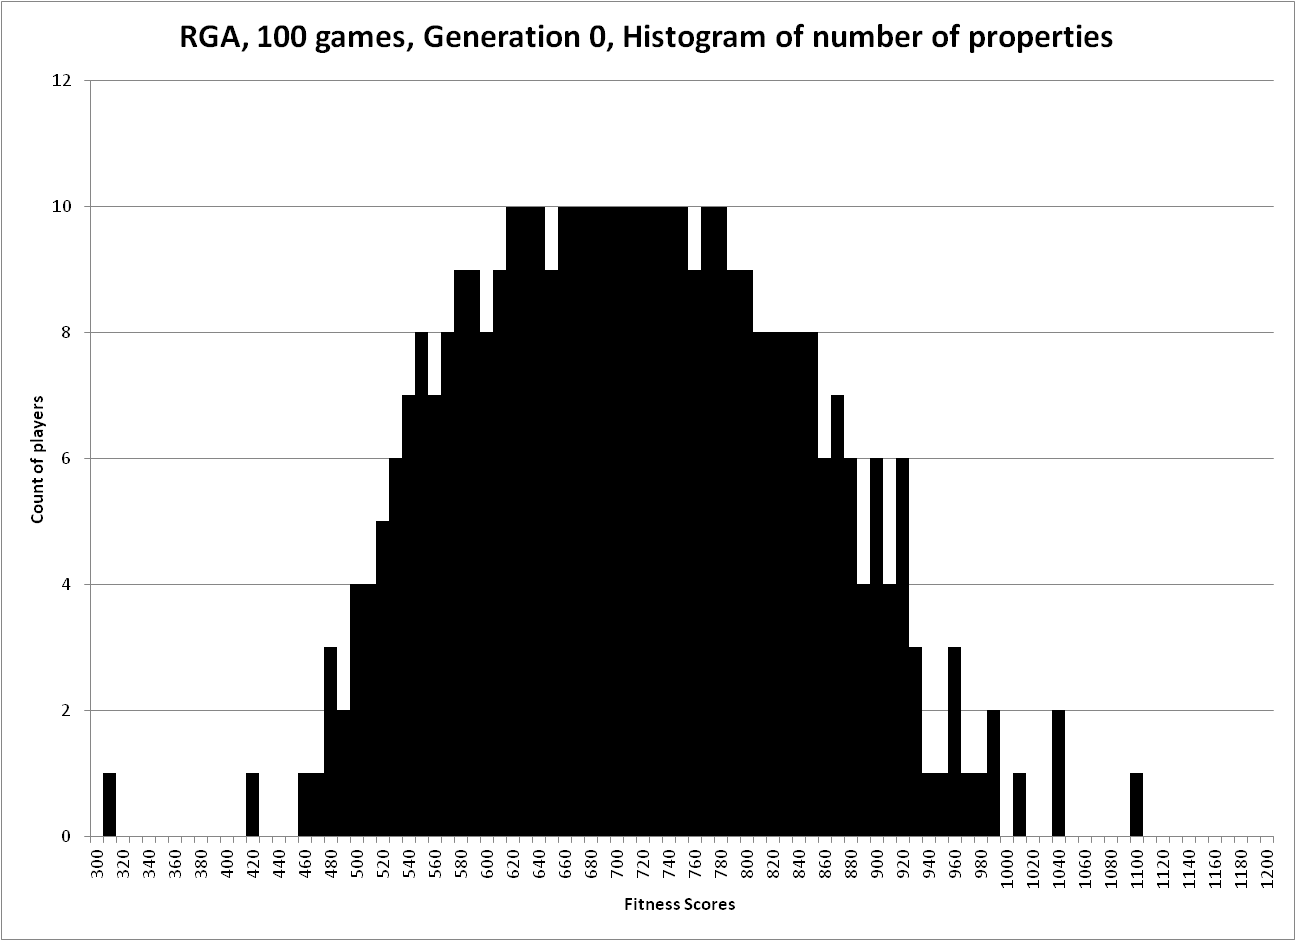
\includegraphics[width=1.0\linewidth]{Figures/RGA_1024_G000_N100_NP.png}
\caption[RGA Num Properties Fitness Distribution, Initial Generation]{RGA
chromosome, size 1024, 100 games per generation, number of properties fitness
evaluator, generation 0.}
\label{figure-RGA-G000-N100-NP-initial_fitness}

\end{minipage}
\end{figure}

Example fitness distributions for the other fitness evaluators are shown in
Figure~\ref{figure-RGA-G000-N100-NetW-initial_fitness},
Figure~\ref{figure-RGA-G000-N100-NM-initial_fitness}, and
Figure~\ref{figure-RGA-G000-N100-NP-initial_fitness}. The distribution for
TOURNAMENT is not shown because it does not follow the same pattern. For
TOURNAMENT, half the population has a score of 0, half of the remainder has a
score of 1, etc., until the final two players have a score of \(log_{2} n-1\).
The TOURNAMENT population will be examined in detail in the validation section.

All of the other populations, regardless of population size, fitness evaluator,
or number of games per generation, show similar results for the initial
generation. These fitness distributions are not surprising. Three of the fitness
evaluators are competitive fitness functions (NUM\_MONOPOLIES and
NUM\_PROPERTIES are not directly competitive, since the player with the most
monopolies or properties is not necessarily the winner of the game). The fact
that the results match previous research into competitive fitness functions
shows that the evolutionary approach we have taken appears to be correct.

\subsection{Results for Subsequent RGA Generations}

As the players get better and the population is more evenly matched, most
players will tend to win half the games they play. As poor players are removed
from the population, the remaining players will tend to be nearer each other in
``ability.'' Thus, the distribution of fitness scores will become much tighter
around the average score, and no single player will be able to dominate the
other players.

For an example of this we look at generation 100 of the RGA-1024-100-FO
population. Figure~\ref{figure-100th_gen_fitness} shows the actual fitness
distribution for this population. The mean remained the same, but the variance
has appeared to decrease. Whereas the fitness scores in generation 0 ranged from
103 to 193, in generation 100 they ranged from 115 to 186. The distribution
around the mean tightened relatively quickly (it can clearly be seen in
generation 100), and then remained fairly constant over the course of the
simulation which was 1000 generations.

\begin{figure}[htp]
\centerline{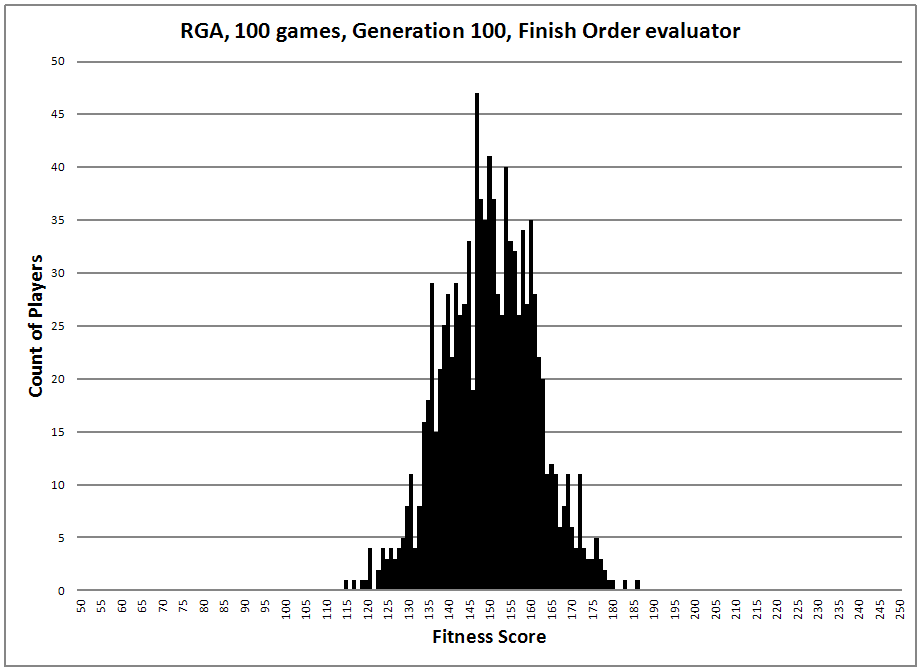
\includegraphics[width=0.75\columnwidth]{Figures/RGA_1024_G100_N100_FO.png}}
\caption[RGA Fitness Distribution, 100th Generation]{RGA chromosome, generation
100, 100 games per generation, finish order fitness evaluator.}
\label{figure-100th_gen_fitness}
\end{figure}

Additional plots of the distribution of fitness scores can be seen in
Figure~\ref{figure-RGA-250th_gen_fitness},
Figure~\ref{figure-RGA-500th_gen_fitness},
Figure~\ref{figure-RGA-750th_gen_fitness}, and
Figure~\ref{figure-RGA-999th_gen_fitness}. Each of these figures shows the
RGA-1024-100-FO population at various points in the evolution process.

\begin{figure}
\centering
%%----start of first figure----
\begin{minipage}[t]{0.47\linewidth}
\centering
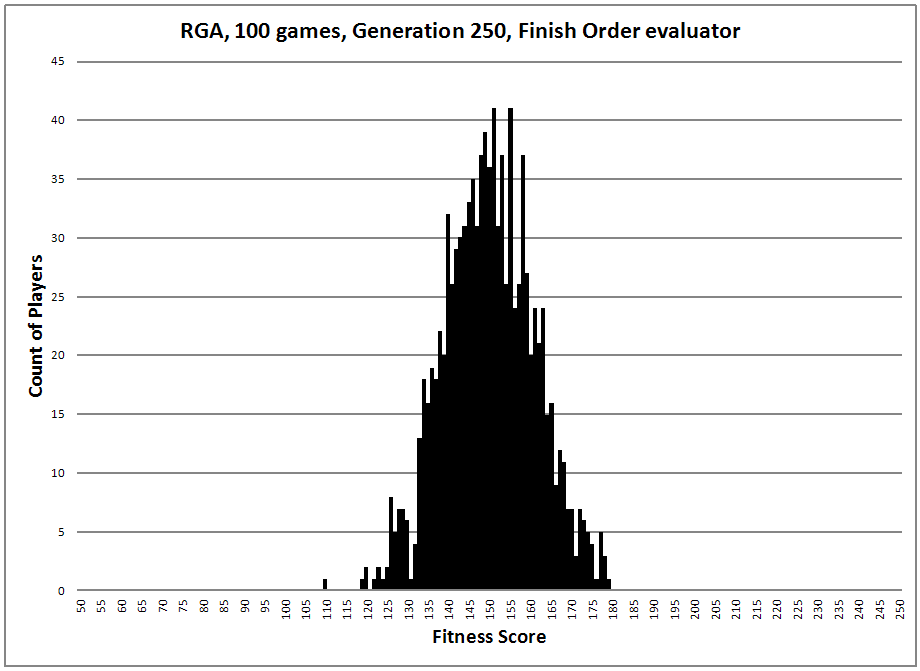
\includegraphics[width=1.0\linewidth]{Figures/RGA_1024_G250_N100_FO.png}
\caption[RGA Fitness Distribution, 250th Generation]{RGA chromosome, size 1024,
100 games per generation, finish order fitness evaluator, generation
250.}
\label{figure-RGA-250th_gen_fitness}
\end{minipage}%
\hspace{0.06\linewidth}%
%%----start of second figure----
\begin{minipage}[t]{0.47\linewidth}
\centering
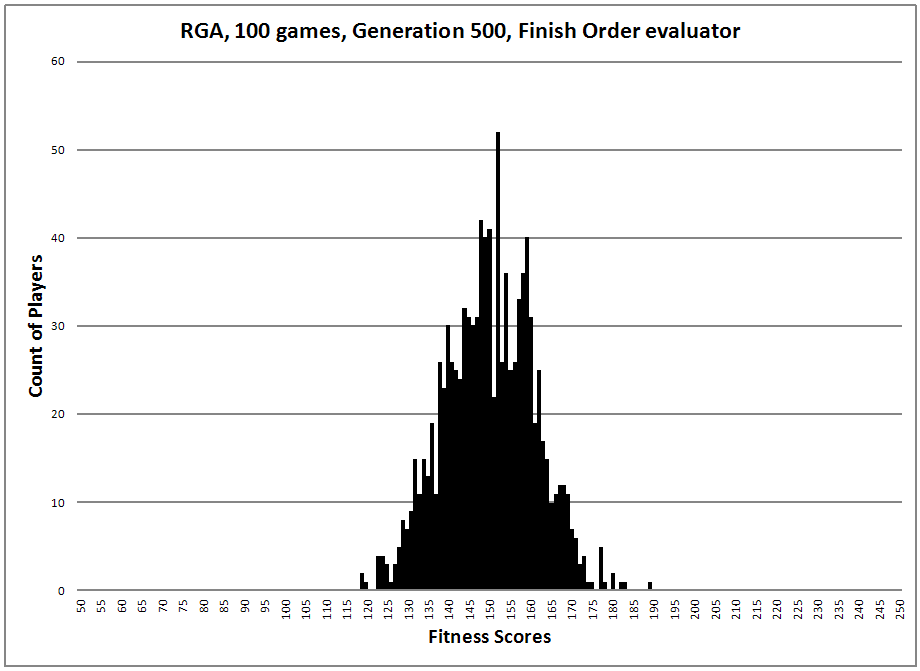
\includegraphics[width=1.0\linewidth]{Figures/RGA_1024_G500_N100_FO.png}
\caption[RGA Fitness Distribution, 500th Generation]{RGA chromosome, size 1024,
100 games per generation, finish order fitness evaluator, generation
500.}
\label{figure-RGA-500th_gen_fitness}
\end{minipage}

\begin{minipage}[t]{0.47\linewidth}
\centering
%%----start of third figure----
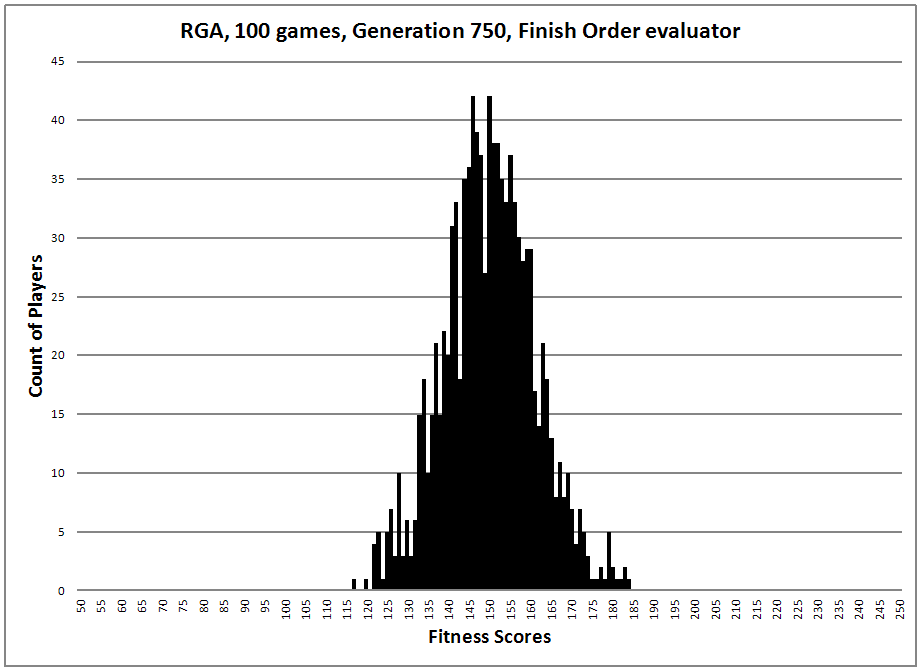
\includegraphics[width=1.0\linewidth]{Figures/RGA_1024_G750_N100_FO.png}
\caption[RGA Fitness Distribution, 750th Generation]{RGA chromosome, size 1024,
100 games per generation, finish order fitness evaluator, generation
750.}
\label{figure-RGA-750th_gen_fitness}
\end{minipage}%
\hspace{0.06\linewidth}%
%%----start of fourth figure----
\begin{minipage}[t]{0.47\linewidth}
\centering
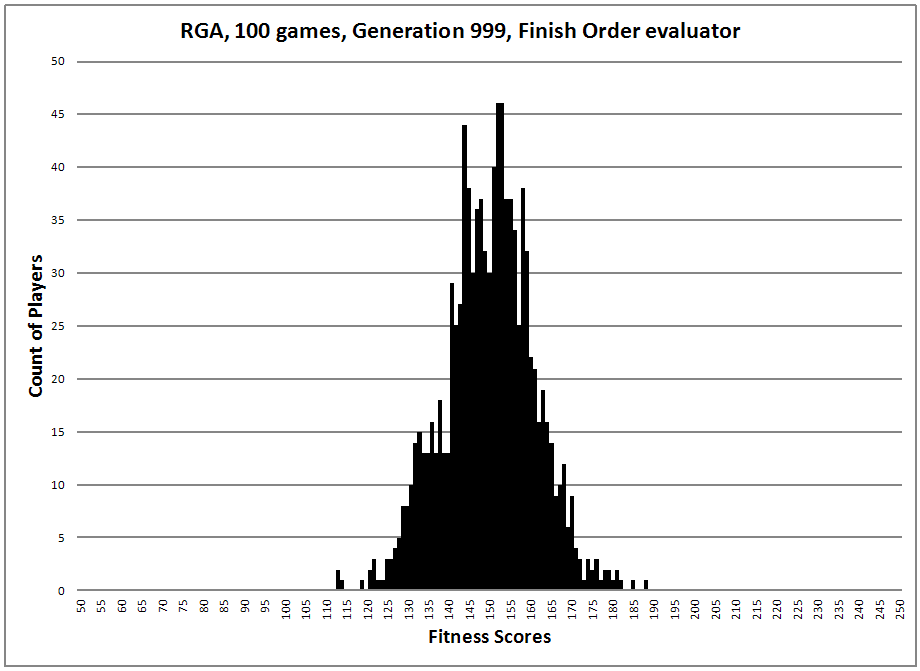
\includegraphics[width=1.0\linewidth]{Figures/RGA_1024_G999_N100_FO.png}
\caption[RGA Fitness Distribution, 999th Generation]{RGA chromosome, size 1024,
100 games per generation, finish order fitness evaluator, generation
999.}
\label{figure-RGA-999th_gen_fitness}
\end{minipage}
\end{figure}

Inspecting Figures~\ref{figure-RGA-250th_gen_fitness} through
\ref{figure-RGA-999th_gen_fitness}, it appears that at some point between the
100th generation and the 250th generation\footnote{Because of the large amount
of data generated by the simulations, data for every generation was not output
by the simulation. Instead fitness data was output and saved for the initial
population, the 100th generation, and every 250th generation. Thus, the point at
which the population average fitness reaches the plateau cannot be calculated.
However, in a coevolutionary environment this is not a problem. A coevolutionary
population can continue to improve even though the fitness appears to plateau.
This will be further discussed later in this Chapter.} that the population
average fitness reaches a plateau. This is also demonstrated by looking at some
of the descriptive statistics for each generation. These are shown in
Table~\ref{table-stats-for-s1024-n100-fo} for the RGA-1024-100-FO population.

\begin{table}[ht]
\begin{center}
\caption[RGA-1024-100-FO statistics]{Descriptive statistics for RGA-1024-100-FO}
\begin{tabular}{ | r || r | r | r | r | r |}
\hline
Generation & Min & Max & Average & Variance & Std Dev \\ \hline \hline
0   & 103 & 193 & 150 & 227.43 & 15.08 \\ \hline
100 & 115 & 186 & 150 & 126.81 & 11.26 \\ \hline
250 & 110 & 179 & 150 & 122.02 & 11.05 \\ \hline
500 & 119 & 189 & 150 & 120.44 & 10.97 \\ \hline
750 & 117 & 184 & 150 & 124.63 & 11.16 \\ \hline
999 & 113 & 188 & 150 & 121.10 & 11.00 \\ \hline
\end{tabular}
\label{table-stats-for-s1024-n100-fo}
\end{center}
\end{table}

In the initial generation, the standard deviation is 15.08, drops to 11.26 by
the 100th generation, and then in the remaining generations (250, 500, 750, and
999) the standard deviation appears to fluctuate around 11.05. We did not
attempt to determine whether this difference in variance between generations is
statistically significant\footnote{To test the hypothesis that the standard
deviations are not equal between generations would require running (in this
example) a population of size 1024 through at least 250 generations, and then
repeating that 250 generation trial enough times to get a statistically
significant sample. Based on the work performed for this research, doing this
for the all of the populations would have taken several weeks of processing
time. It was decided that a better use of resources would be to do a comparative
test between players of different generations and populations.}.

Additional population statistics are in
Table~\ref{table-stats-for-s1024-n100-netw} for the RGA-1024-100-NetW
population, Table~\ref{table-stats-for-s1024-n100-nm} for the RGA-1024-100-NM
population, Table~\ref{table-stats-for-s1024-n100-np} for the RGA-1024-100-NP
population, and Table~\ref{table-stats-for-s1024-n100-nw} for the
RGA-1024-100-NW population.

\begin{table}[ht]
\begin{center}
\caption[RGA-1024-100-NetW statistics]{Descriptive statistics for RGA-1024-100-NetW}
\begin{tabular}{ | r || r | r | r | r | r |}
\hline
Generation & Min & Max & Average & Variance & Std Dev \\ \hline \hline
0   & 4728 & 11186 & 7499.99 & 1137919.23 & 1066.73 \\ \hline
250 & 4285 & 10374 & 7499.80 &  649447.67 &  805.88 \\ \hline
500 & 5235 & 10242 & 7500.00 &  665909.43 &  816.03 \\ \hline
750 & 5080 & 10977 & 7500.05 &  723209.97 &  850.42 \\ \hline
999 & 5306 &  9831 & 7499.96 &  649001.83 &  805.61 \\ \hline
\end{tabular}
\label{table-stats-for-s1024-n100-netw}
\end{center}
\end{table}

\begin{table}[ht]
\begin{center}
\caption[RGA-1024-100-NM statistics]{Descriptive statistics for RGA-1024-100-NM}
\begin{tabular}{ | r || r | r | r | r | r |}
\hline
Generation & Min & Max & Average & Variance & Std Dev \\ \hline \hline
0   &  8 & 209 &  80.42 & 1014.77 & 31.86 \\ \hline
250 & 37 & 226 & 110.88 &  758.92 & 27.55 \\ \hline
500 & 43 & 199 & 111.20 &  707.89 & 26.61 \\ \hline
750 & 44 & 199 & 113.97 &  732.09 & 27.06 \\ \hline
999 & 17 & 217 & 116.52 &  734.49 & 27.10 \\ \hline
\end{tabular}
\label{table-stats-for-s1024-n100-nm}
\end{center}
\end{table}

\begin{table}[ht]
\begin{center}
\caption[RGA-1024-100-NP statistics]{Descriptive statistics for RGA-1024-100-NP}
\begin{tabular}{ | r || r | r | r | r | r |}
\hline
Generation & Min & Max & Average & Variance & Std Dev \\ \hline \hline
0   & 309 & 1094 & 698.18 &  10271.47 & 101.35 \\ \hline
250 & 504 &  929 & 697.75 &   5322.08 &  72.95 \\ \hline
500 & 478 &  973 & 697.72 &   6126.09 &  78.27 \\ \hline
750 & 462 &  983 & 697.81 &   5928.88 &  77.00 \\ \hline
999 & 438 & 1007 & 697.79 &   6095.32 &  78.07 \\ \hline
\end{tabular}
\label{table-stats-for-s1024-n100-np}
\end{center}
\end{table}

\begin{table}[ht]
\begin{center}
\caption[RGA-1024-100-NW statistics]{Descriptive statistics for RGA-1024-100-NW}
\begin{tabular}{ | r || r | r | r | r | r |}
\hline
Generation & Min & Max & Average & Variance & Std Dev \\ \hline \hline
0   & 27 & 126 & 75.00 & 286.43 & 16.92 \\ \hline
250 & 36 & 120 & 75.00 & 155.68 & 12.48 \\ \hline
500 & 30 & 117 & 75.00 & 168.21 & 12.97 \\ \hline
750 & 39 & 120 & 75.00 & 160.36 & 12.66 \\ \hline
999 & 30 & 114 & 75.00 & 173.74 & 13.18 \\ \hline
\end{tabular}
\label{table-stats-for-s1024-n100-nw}
\end{center}
\end{table}

In all of the tables, the average population fitness stays approximately
the same, and the variance in population fitness decreases. Even though it
appears that the variance has plateaued in these examples, players in later
generations can still be improving in fitness. In fact, we show later in this
chapter that players in the last generation are statistically better (i.e., they
win more games) than players in the earliest generations.

This section has focused primarily on the RGA-1024-100 sets of populations. In
general, a similar pattern of statistics is seen in most of the other RGA and
TGA populations that were evolved in this study. Some of the populations,
however, showed weaker, or sometimes conflicting results. A complete set of
tables with that information for the RGA populations can be found in
Appendix~\ref{appendix:rgastats}.

The populations that did not appear to improve over time were the populations
with small population size or small numbers of games per generation. One example
is shown in Table~\ref{tab:6_RGA-0032-007-FO}. In this case, the population
variance gets larger over time, which implies that this population improved
little or none from the first generation to the last. Section~\ref{6_Validation}
provides details on whether the populations did improve or not.

\begin{table}[htbp]
  \centering
  \caption[RGA-0032-007-FO Statistics]{Descriptive Statistics for RGA-0032-007-FO}
    \begin{tabular}{lrrrrrr}
    \toprule
    Population &  Generation & Min    & Max    & Average & Variance & Std Dev \\
    \midrule
    RGA-0032-007-FO & 0      & 4      & 16     & 10.50  & 8.77   & 2.96 \\
    RGA-0032-007-FO & 250    & 4      & 17     & 10.50  & 9.23   & 3.04 \\
    RGA-0032-007-FO & 500    & 5      & 16     & 10.50  & 10.13  & 3.18 \\
    RGA-0032-007-FO & 750    & 2      & 19     & 10.50  & 12.71  & 3.57 \\
    RGA-0032-007-FO & 999    & 5      & 16     & 10.50  & 10.26  & 3.20 \\
    \bottomrule
    \end{tabular}
  \label{tab:6_RGA-0032-007-FO}%
\end{table}%

\subsection{Genome Changes Over Time}

We now look at the change in a genome between the initial and final
generations of a population. Using the RGA-1024-100-FO population, part of
the genome for the best player from generation 0 is shown in
Figure~\ref{figure-genome0} and part of the genome for the best player from
generation 999 is shown in Figure~\ref{figure-genome999}. For easier comparison,
the chromosome values from the chart are also shown in
Table~\ref{tab:chromo_compare}.

\begin{figure}[htp]
\centerline{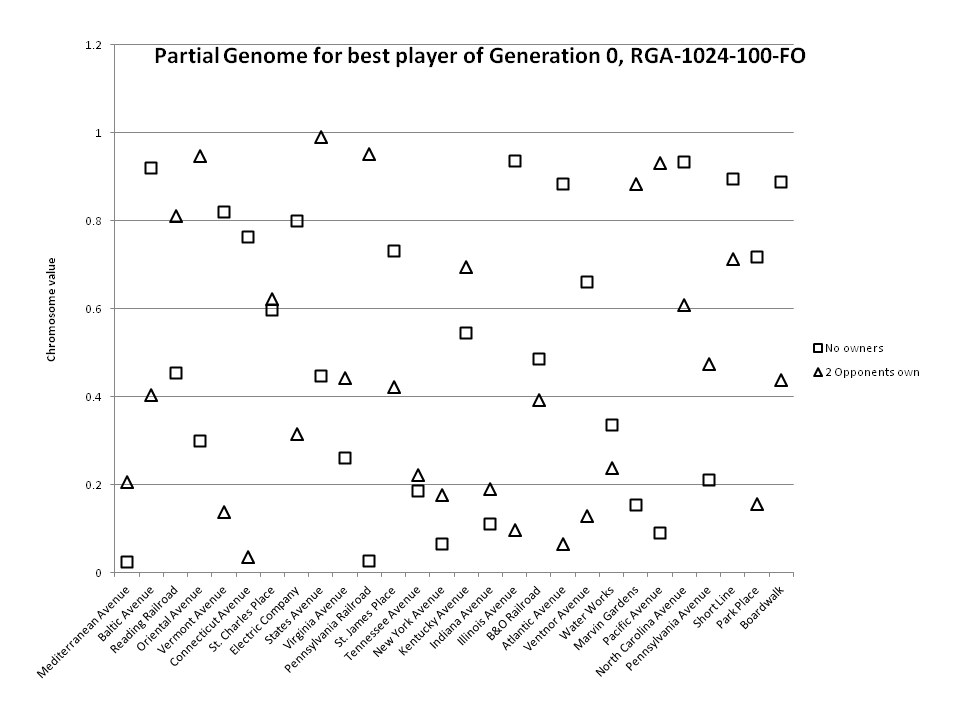
\includegraphics[width=0.75\columnwidth]{Figures/genome000.png}}
\caption[Illustration of Genome, Generation 0]{This chart shows part of the
genome of the fittest player in the first generation of the RGA-1024-100-FO
population. This chart compares the chromosome used when no player owns
any property in the group (represented by the square symbol) against the
chromosome used when two other players own a property in the group (the triangle
symbol).}
\label{figure-genome0}
\end{figure}

\begin{figure}[htp]
\centerline{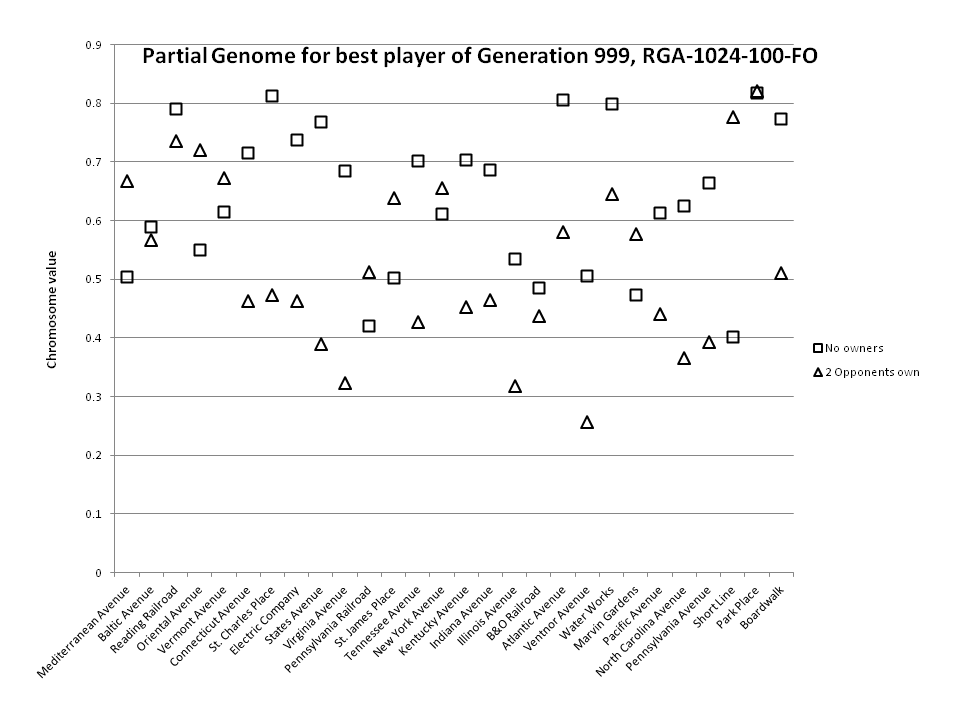
\includegraphics[width=0.75\columnwidth]{Figures/genome999.png}}
\caption[Illustration of Genome, Generation 999]{This chart shows part of the
genome of the fittest player in the last generation of the RGA-1024-100-FO
population. This chart compares the chromosome used when no player owns any
property in the group (the square symbol) against the chromosome used when two
other players own a property in the group (the triangle symbol). These two genes
show agreement with the heuristic strategy: the player is more likely to buy a
property when no one owns a property in the group, and relatively less likely to
buy a property when other players are blocking the group from being
monopolized.}
\label{figure-genome999}
\end{figure}

% Table generated by Excel2LaTeX from sheet 'genome0099 (2)'
\begin{table}[htbp]
  \centering
  \caption[Genome Comparison, Gen 0 vs Gen 999]{Comparison of Best Genomes from Generation 0 and Generation 999}
  \scalebox{0.75}{
    \begin{tabular}{lrrr|rrr}
    \toprule
           & \multicolumn{3}{c|}{Generation 0} & \multicolumn{3}{c}{Generation 999} \\
    \midrule
           & No Owner & 2 Opponents own & Diff   & No Owner & 2 Opponents own & Diff \\
    Mediterranean Avenue & 0.023  & 0.205  & -0.182 & 0.504  & 0.668  & -0.164 \\
    Baltic Avenue & 0.920  & 0.404  & 0.517  & 0.589  & 0.567  & 0.023 \\
    Reading Railroad & 0.454  & 0.810  & -0.356 & 0.790  & 0.736  & 0.054 \\
    Oriental Avenue & 0.300  & 0.947  & -0.648 & 0.550  & 0.721  & -0.171 \\
    Vermont Avenue & 0.821  & 0.138  & 0.683  & 0.614  & 0.673  & -0.059 \\
    Connecticut Avenue & 0.762  & 0.036  & 0.726  & 0.715  & 0.463  & 0.252 \\
    St. Charles Place & 0.598  & 0.622  & -0.024 & 0.812  & 0.473  & 0.339 \\
    Electric Company & 0.799  & 0.314  & 0.484  & 0.737  & 0.463  & 0.274 \\
    States Avenue & 0.448  & 0.991  & -0.543 & 0.768  & 0.389  & 0.379 \\
    Virginia Avenue & 0.260  & 0.442  & -0.182 & 0.685  & 0.323  & 0.362 \\
    Pennsylvania Railroad & 0.027  & 0.952  & -0.925 & 0.421  & 0.512  & -0.091 \\
    St. James Place & 0.730  & 0.423  & 0.308  & 0.502  & 0.639  & -0.137 \\
    Tennessee Avenue & 0.186  & 0.223  & -0.036 & 0.702  & 0.427  & 0.275 \\
    New York Avenue & 0.064  & 0.175  & -0.111 & 0.612  & 0.656  & -0.043 \\
    Kentucky Avenue & 0.544  & 0.694  & -0.150 & 0.704  & 0.452  & 0.252 \\
    Indiana Avenue & 0.110  & 0.189  & -0.080 & 0.686  & 0.465  & 0.221 \\
    Illinois Avenue & 0.936  & 0.096  & 0.840  & 0.536  & 0.319  & 0.217 \\
    B\&O Railroad & 0.487  & 0.391  & 0.095  & 0.485  & 0.437  & 0.048 \\
    Atlantic Avenue & 0.884  & 0.064  & 0.820  & 0.806  & 0.581  & 0.225 \\
    Ventnor Avenue & 0.661  & 0.128  & 0.532  & 0.506  & 0.257  & 0.250 \\
    Water Works & 0.335  & 0.237  & 0.098  & 0.800  & 0.645  & 0.154 \\
    Marvin Gardens & 0.154  & 0.883  & -0.730 & 0.472  & 0.577  & -0.104 \\
    Pacific Avenue & 0.091  & 0.931  & -0.840 & 0.614  & 0.440  & 0.173 \\
    North Carolina Avenue & 0.934  & 0.609  & 0.325  & 0.625  & 0.365  & 0.260 \\
    Pennsylvania Avenue & 0.210  & 0.474  & -0.265 & 0.663  & 0.392  & 0.271 \\
    Short Line & 0.895  & 0.713  & 0.182  & 0.402  & 0.778  & -0.376 \\
    Park Place & 0.718  & 0.155  & 0.563  & 0.818  & 0.822  & -0.004 \\
    Boardwalk & 0.887  & 0.439  & 0.448  & 0.774  & 0.511  & 0.263 \\
    \bottomrule
    \end{tabular}}
  \label{tab:chromo_compare}%
\end{table}%

It can be seen that in general, for the property buying decision, the genome
matches the strategy described previously. The gene values for buying a location
are higher when no player owns one of the properties of a group compared to when
two other players own properties in the group. Although it is not shown in
Figure~\ref{figure-genome999}, the gene values for buying when the player
already owns a property in the group, or when one opponent owns a property in
the group, are generally higher than when two opponents own a property in the
group. A few additional Figures and Tables for some genomes can be found in
Appendix~\ref{appendix:chromos}.

When compared to the strategy list from~\ref{m_gamestrategies}, there might
appear to be an inconsistency in the genome. For example, the strategy says
always buy a property if no one else owns a property in the same group. However,
the greatest gene value in the genome from generation 999 is for Park Place at
0.82. This can easily be explained by the fact that if the player declines a
property with probability \(p_{decline} = 1-p_{buy}\), the probability of
subsequently buying the property is higher. This is because when a player
declines a property, it is then auctioned to any player including the declining
player, and the declining player uses the same chromosome to make the bid
decision independently of the buy decision. So the probability of deciding to
buy a property is
\begin{equation*}
1-(p_{decline} \cdot p_{decline})
\end{equation*}
For example, the probability of a player deciding to buy Park Place with a
chromosome of 0.82 is
\begin{equation*}
1-(0.18 \cdot 0.18) \approx 0.97
\end{equation*}
The probability of actually obtaining the property is slightly lower, however,
since it is dependent on winning the auction.

\subsection{SGA Players} \label{6_SGA}

After evolving the population of RGA Players, the simulation was conducted again
using SGA Players. SGA players are those players with a binary string
chromosome.

The fitness distribution in the first generation shows the same general
similarity to the binomial distribution (Figure~\ref{figure-sga_gen0}), although
there appears to be a bit of skewness.

\begin{figure}[htp]
\centerline{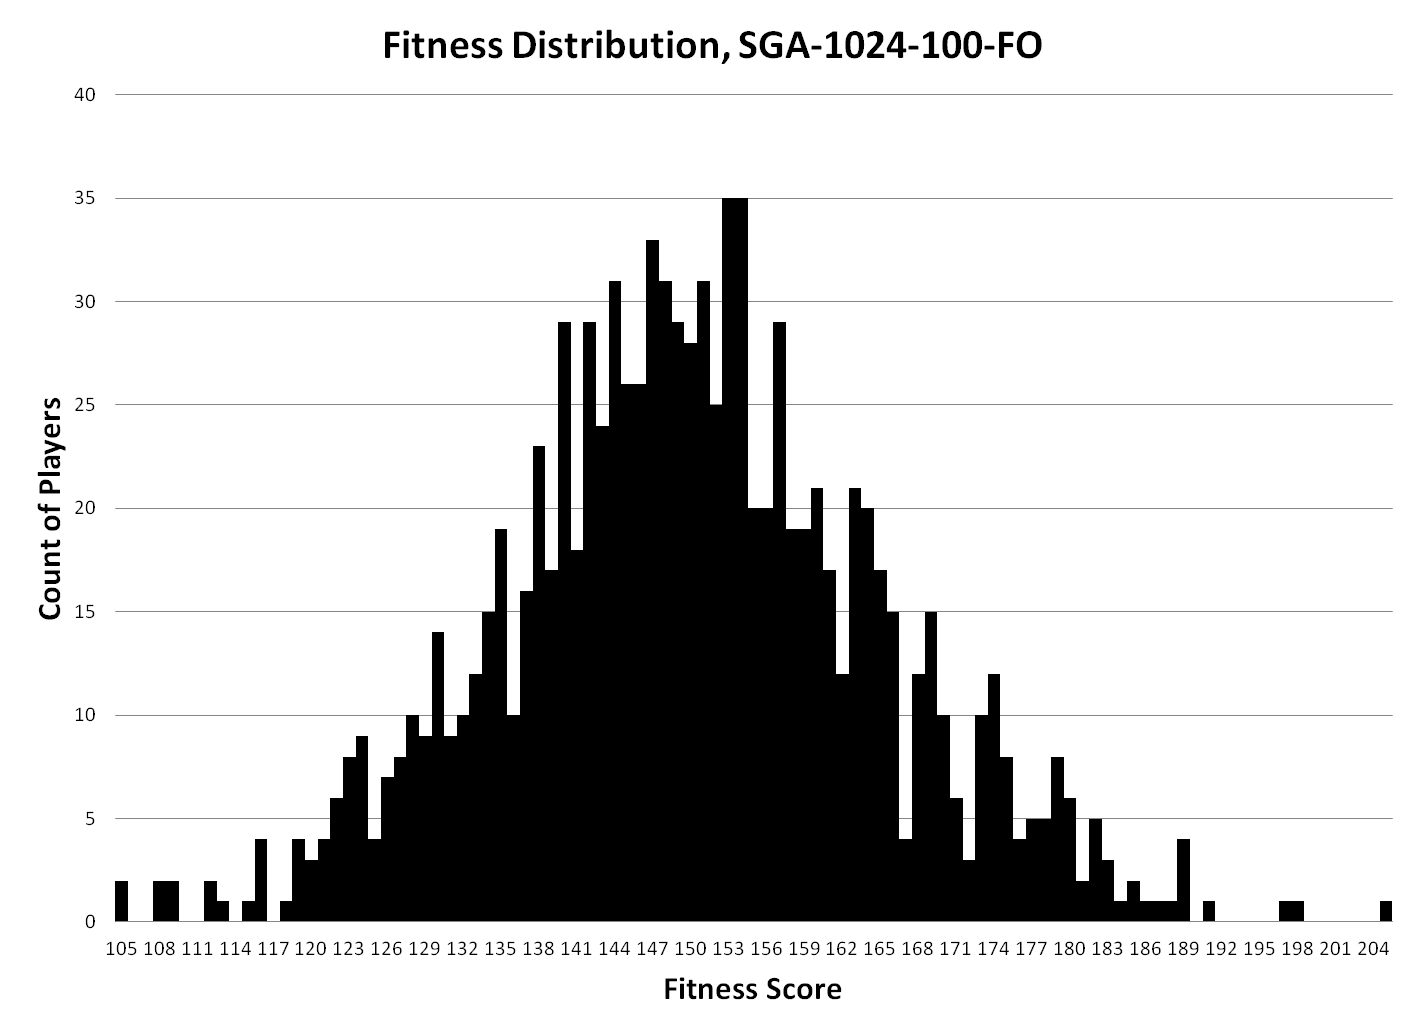
\includegraphics[width=0.75\columnwidth]{Figures/SGA_1024_100_FO_gen0.png}}
\caption[SGA-1024-100-FO Fitness Generation 0]{This figure shows the fitness
distribution for the first generation of the SGA-1024-100-FO population.}
\label{figure-sga_gen0}
\end{figure}

Figure~\ref{figure-sga_gen250} shows the fitness distribution at generation 250
and the skew is definitely present.

\begin{figure}[htp]
\centerline{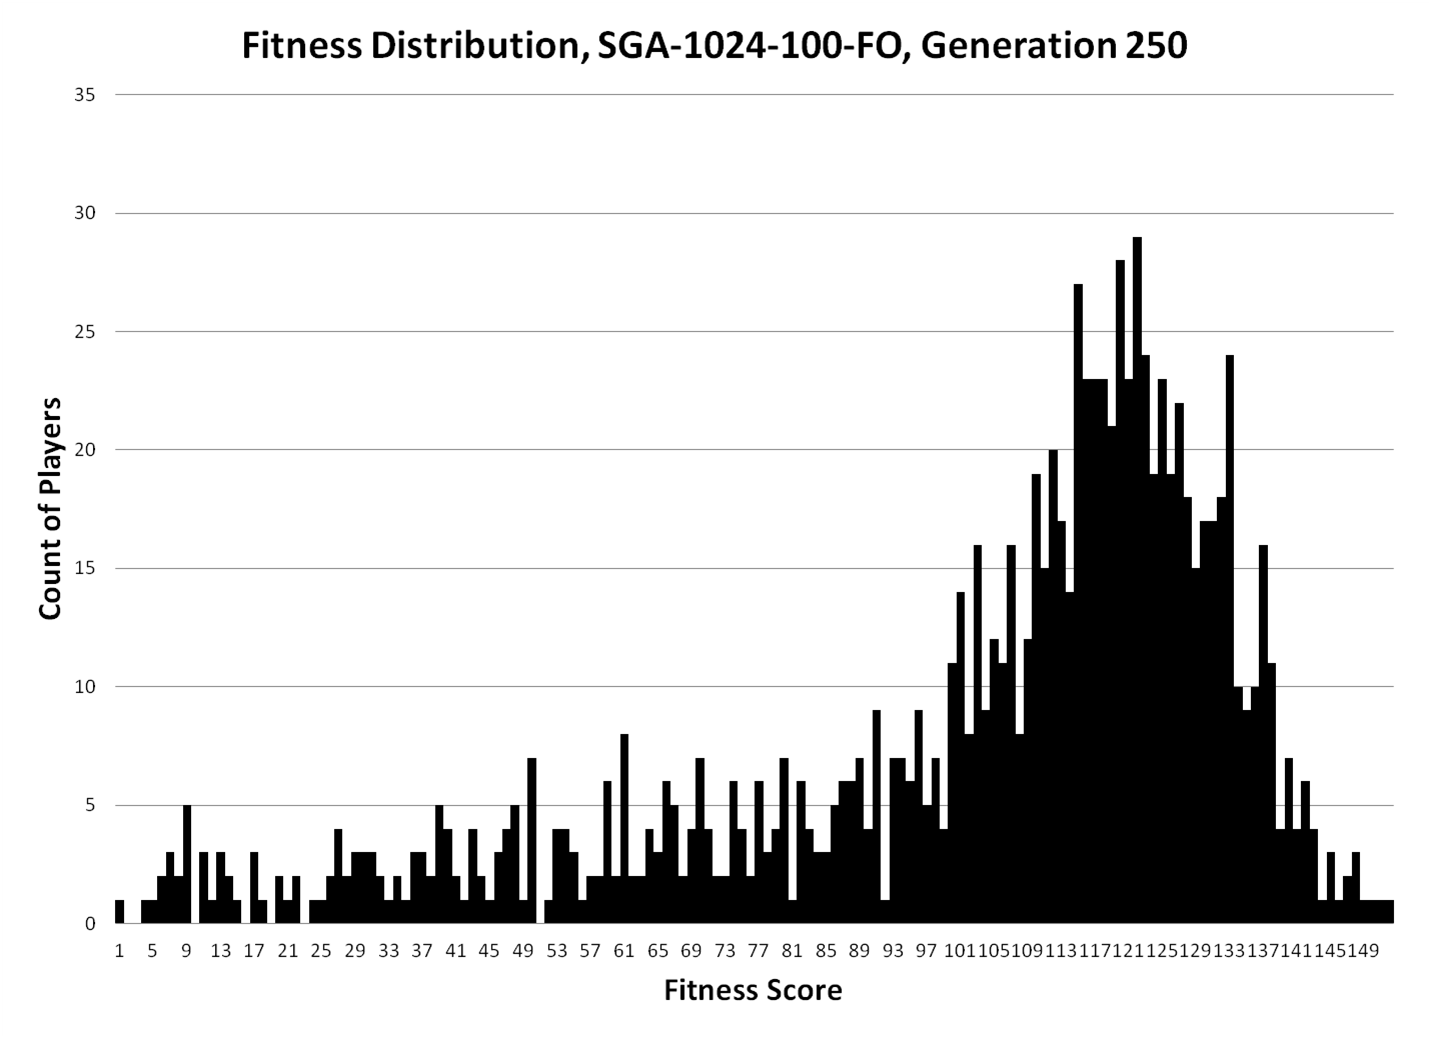
\includegraphics[width=0.75\columnwidth]{Figures/SGA_1024_100_FO_gen250.png}}
\caption[SGA Fitness Generation 289]{This chart shows the fitness
distribution for generation 250 of the SGA-1024-100-FO population.}
\label{figure-sga_gen250}
\end{figure}

Although not shown in this thesis, Generations 500 and 750, for the
SGA-1024-100-FO population, show the same general fitness distribution: a long
tail of low fitness scores, with a peak at higher scores. The fitness
distribution for Generation 999 shows the same pattern and can be seen in
Appendix~\ref{appendix:SGAFitness}.

Appendix~\ref{appendix:SGAFitness} also contains sample fitness distributions
from other SGA populations. They all show the same pattern. At generation 0,
they are generally symmetric, but sometime prior to generation 250, the
distribution skews so that there is a long tail of low fitness scores, and a
peak of scores higher than the expected average.

At the start of this research, the author thought that the SGA chromosomes would
perform as well as the RGA or TGA chromosomes. Early researchers in genetic
algorithms thought that simple chromosomes would work for most, if not all
problems~\cite{goldberg1989genetic}.

Not only did the fitness distributions show problems, but some initial play
testing of a few of the ``best'' SGA players showed that they performed much
more poorly than the RGA and TGA players, losing in every trial. It was only
after this that we found the following from Fogel~\cite{fogel1999intelligence}:

\begin{quote}
We must also admit that several previous theoretical speculations in
evolutionary computation have proven to be incorrect. \ldots~Davis (1991),
Michalewicz (1992), B\"ack and Schwefel (1993), Fogel and Stayton (1994), and
many others, have reported better and faster results in continuous optimization
problems when using real-valued representations instead of bit strings. \ldots
so the proper conclusion is to use the representation that follows naturally
from the problem and gives you the best insight into discovering improved
solutions.
\end{quote}

Based on the poor results of the SGA players, and the conclusion that the
chromosome for a problem should not automatically be a bit string, but should be
one best suited to the problem domain, the effort to improve or validate the SGA
chromosome players was no longer pursued as part of this research.

\subsection{TGA Players} \label{6_TGS}

Finally, the same simulation and evolution was conducted using TGA players. The
results for the TGA player were essentially the same as for the RGA player.

The fitness distributions for the initial populations had the same shape as a
binomial distribution, with similar minimums and maximums for the initial
generation as for the RGA chromosomes. Over the 1000 generation simulations, the
fitness distribution converged towards the mean fitness. The minimum, maximum,
mean, and median were essentially the same as the RGA simulation, and the player
genomes were also very similar. This is unsurprising, since the fitness seems to
depend mostly on buying property (in which the RGA and TGA genomes are
identical), and not on getting out of jail which was the difference between the
two genomes.

For this reason, no further validation of the TGA players was pursued. Instead,
the remainder of the study effort focused on validating the RGA players. This
validation is discussed in the next section.

\section{Population Validation} \label{6_Validation}

As with other research that used competitive fitness functions, validations of
the various populations were performed to test if the populations were actually
getting better.

\subsection{Intrapopulation validation}

For every population, the best player in generation 999 was played against
the best player in generations 250, 500, and 750. 100 games were played with the
same set of 4 best players. If the population was actually evolving better
players, we expect that on average, the best player in the last generation will
win more games then the other players; and the best player in the 250th
generation should lose more games on average.

After 100 games were played, this same trial was repeated 50 times, without
evolution. At the start of validation, 50 games repeated for 100 trials was
chosen to ensure statistically significant results.

Appendix~\ref{appendix:intravalidation} presents the complete set of results for
the RGA-0128 and the RGA-1024 populations. What the tables in the appendix show
is that the populations did improve over time, at least when played against each
other. Table~\ref{tab:validationRGA0128} is an excerpt of the validation results
for the RGA-0128 population (the complete table is in the appendix).

% Table generated by Excel2LaTeX from sheet 'Finish Order'
\begin{table}[htbp]
  \centering
  \caption{Intrapopulation validation, population size 128, Evaluated by finish order}
    \begin{tabularx}{\linewidth}{|p{1in}|p{1in}|r|r|r|r|r|}
    \cline{3-7}
    \multicolumn{1}{l}{} &  & \multicolumn{2}{c|}{Avg fitness} & \multicolumn{3}{c|}{One tailed t test} \\
    \cline{1-7}
    Number of games per generation in original population
    & Original fitness evaluator
    & \multicolumn{1}{p{0.7in}|}{Generation 250}
    & \multicolumn{1}{p{0.7in}|}{Generation 500}
    & \multicolumn{1}{X|}{t test G250 vs G500}
    & \multicolumn{1}{X|}{t test G500 vs G750}
    & \multicolumn{1}{X|}{t test G750 vs G999} \\
    \cline{1-7}
      \multirow{5}{*}{100}
      & finish order & 1389.42 & 1489.52 & 0.0000 & 0.0000 & 0.0000 \\
      \cline{2-7}
      & net worth & 1426.96 & 1472.62 & 0.0000 & 0.0000 & 0.0000 \\
      \cline{2-7}
      & num monop & 1464.06 & 1494.22 & 0.0001 & 0.1532 & 0.0000 \\
      \cline{2-7}
      & num props & 1438.08 & 1487.34 & 0.0000 & 0.0003 & 0.0000 \\
      \cline{2-7}
      & num wins & 1418.00 & 1493.70 & 0.0000 & 0.0000 & 0.0403 \\
      \cline{1-7}
    \end{tabularx}%
  \label{tab:validationRGA0128}%
\end{table}%

Each row represents a single population. The first row, for example, is the
RGA-0128-100-FO population. The best player from generations 250, 500, 750, and
999 were competed against each other. In these trials, the fitness of each
player is evaluated using finish order evaluator. The score in the average
fitness column is the average fitness scores for that player over 50 trials of
100 games per trial. To evaluate whether players in later generations were
better than players in earlier generations, a one-tailed Student's t-test was
performed with $H_{0}$ that the average fitness is the same for each generation.
In most cases, the null hypothesis is rejected, indicating that the average
fitness scores are different. Since average fitness increases over time, the
one-tailed t-test says that not only are the fitness scores different, the
average fitness is increasing over time.

The table above shows 3 of the tests: generation 250 compared to generation 500,
500 to 750, and 750 to 999. At almost any significance level, the results
indicate that almost every later generation is better than every earlier
generation. One of the exceptions in the table above is for the NUM\_MONOPOLIES
evaluator in the comparison of generation 500 to generation 750. For that test
we accept the null hypothesis and must conclude that the players from those two
generations have the same ability.

However, looking at all the results in Appendix~\ref{appendix:intravalidation},
we reject the null hypothesis for most of the tests.

Where we tend to accept the null hypothesis most often is for populations with
a small number of games per generation, and for populations that are temporally
close to each other. For example, looking at the RGA-0128 table in the Appendix,
when the number of games per generation is 7, The null hypothesis is accepted
14 out of 25 trials at the 0.05 significance level. Looking at the same table,
the null hypothesis is accepted most often when comparing Generation 500 to 750
(accepted 9 times), and when comparing Generation 750 to 999 (accepted 8 times).

The conclusion from this set of experiments is that better players evolved in
larger populations that played large numbers of games per generation.

\subsection{Interpopulation validation}

Next, the best players from the last generation of similar populations that used
different fitness evaluators were played against each other. This was done to
see which, if any, fitness evaluator produced better players. Because of the
highly random nature of the game and based on the previous work comparing
competitive fitness functions, we expected that the TOURNAMENT fitness evaluator
would produce less fit players than at least some of the other fitness
evaluators.

RESULTS PENDING

\section{Human versus RGA competition}

Based on the results of the evolutionary phase of this study, a set of RGA
players was selected and competed against human players to validate the
evolutionary results. The results of these competitions is presented here.

The intra- and iter-population analysis showed that the best results came from
populations with high population size, many games per generation, and from the
latest generations of the evolution. For those reasons, players for this
validation were selected from the RGA-1024-100-FO population.

\subsection{Human versus computer validation I}

The first competition was conducted after implementing the trading algorithm
proposed by Yasumura, et al, in ``Negotiation strategy of agents in the MONOPOLY
game~\cite{Yasumura2001Negotiate}.''

The algorithm evaluates the ownership situation of the properties being traded,
and then sums various combinations of gains based on that situation. For
example, if a trade would lead to a Monopoly, the algorithm computes the sum of
3 times the expected long-term gain, and the expected mid- and short-term
gains\footnote{Mid-term is defined as the gain or loss after one trip around the
board; short-term is defined as the gain or loss after one dice roll.}, and
adjusts that by a factor \(\omega\). It then subtracts the short- and mid-term
losses, which are adjusted by the factor \(1-\omega\). When the player would be
the only owner of only one property in a group, then a different combination of
gains is summed (long-term gain is less important in this case).

When \(\omega\) is close to 1, the player values gains and completely ignores
losses; alternately, when \(\omega\) is close to 0, the player is more sensitive
to losses. The algorithm results in a value \(U\) which is the gain (or loss)
from the trade.

If the value \(U\) exceeds some threshold, the player proposes the trade, or
accepts the trade. In their paper, Yasumura, et al, claimed that when their
algorithm was compared to the game play of human experts, the algorithm matched
the humans when gains and losses were balanced \(\omega \approx 0.5\)), and when
the threshold was relatively low (approximately 100).

So the algorithm was implemented with those parameters: \(\omega = 0.5\)), and
threshold of 100.

The best 4 players from generations 250, 500, 750, and 999 of the
RGA-1024-100-FO populations were selected. They then competed in a Monopoly game
player against a single human player. For each game, the game chose 3 RGA
opponents at random. So usually the human player was playing against a mix of
players from the 4 generations. This was done to perform a secondary validation
of the fact that players from later generation should be better than players
from earlier generations. If that was the case as proved in the intra-population
validation, then regardless of how the RGA players played against the human
players in aggregate, the players from generation 999 should still do better
than the players from generation 250.

The results of this initial human versus computer validation are shown in
Table~\ref{tab:human_rga_I}.

      % Table generated by Excel2LaTeX from sheet 'Pivot table'
      \begin{table}[htbp]
        \centering
        \caption[Human versus RGA results, initial]{Results of Human versus RGA
        player competitions, with initial trading algorithm}
          \begin{tabular}{r|rrr}
          \toprule
                 & Results &        &  \\
          \midrule
          Players & Average finish & Average networth & Count of games
          \\ \\
          \multicolumn{1}{l|}{gen250} & 2.8    & 1170.1 & 85.0 \\
          \hline
          \multicolumn{1}{l|}{player0040.dat} & 2.6    & 2207.0 & 26.0 \\
          \multicolumn{1}{l|}{player0191.dat} & 2.5    & 765.2  & 15.0 \\
          \multicolumn{1}{l|}{player0478.dat} & 3.0    & 416.2  & 22.0 \\
          \multicolumn{1}{l|}{player0752.dat} & 3.0    & 974.6  & 22.0 \\ \\
          \multicolumn{1}{l|}{gen500} & 2.8    & 1137.4 & 78.0 \\
          \hline
          \multicolumn{1}{l|}{player0028.dat} & 2.8    & 902.8  & 25.0 \\
          \multicolumn{1}{l|}{player0445.dat} & 2.9    & 1291.4 & 21.0 \\
          \multicolumn{1}{l|}{player0913.dat} & 2.7    & 404.6  & 19.0 \\
          \multicolumn{1}{l|}{player0923.dat} & 2.8    & 2410.8 & 13.0 \\ \\
          \multicolumn{1}{l|}{gen750} & 2.7    & 1367.1 & 92.0 \\
          \hline
          \multicolumn{1}{l|}{player0453.dat} & 2.9    & 332.1  & 28.0 \\
          \multicolumn{1}{l|}{player0474.dat} & 2.6    & 1910.8 & 28.0 \\
          \multicolumn{1}{l|}{player0524.dat} & 2.6    & 1195.1 & 18.0 \\
          \multicolumn{1}{l|}{player0750.dat} & 2.6    & 2303.2 & 18.0 \\ \\
          \multicolumn{1}{l|}{gen999} & 2.9    & 954.7  & 72.0 \\
          \hline
          \multicolumn{1}{l|}{player0101.dat} & 3.0    & 762.1  & 18.0 \\
          \multicolumn{1}{l|}{player0423.dat} & 3.1    & 730.9  & 14.0 \\
          \multicolumn{1}{l|}{player0667.dat} & 2.7    & 1645.2 & 13.0 \\
          \multicolumn{1}{l|}{player0928.dat} & 3.0    & 866.6  & 27.0 \\ \\
          \multicolumn{1}{l|}{human} & 1.6    & 7484.0 & 109.0 \\
          \hline
          \multicolumn{1}{l|}{A} & 1.6    & 7926.6 & 19.0 \\
          \multicolumn{1}{l|}{B} & 1.3    & 9141.6 & 24.0 \\
          \multicolumn{1}{l|}{C} & 2.3    & 5443.4 & 8.0 \\
          \multicolumn{1}{l|}{E} & 1.9    & 6311.3 & 12.0 \\
          \multicolumn{1}{l|}{G} & 2.3    & 3030.3 & 3.0 \\
          \multicolumn{1}{l|}{H} & 1.6    & 7371.2 & 13.0 \\
          \multicolumn{1}{l|}{S} & 1.5    & 7644.7 & 23.0 \\
          \multicolumn{1}{l|}{K} & 1.0    & 11473.0 & 3.0 \\
          \multicolumn{1}{l|}{V} & 2.5    & 5654.5 & 2.0 \\
          \multicolumn{1}{l|}{L} & 2.0    & 0.0    & 1.0 \\
          \multicolumn{1}{l|}{T} & 3.0    & 0.0    & 1.0 \\ \\
          \multicolumn{1}{l|}{Grand Total} & 2.5    & 2748.7 & 436.0 \\
          \bottomrule
          \end{tabular}%
        \label{tab:human_rga_I}%
      \end{table}%

Clearly, for this set of competitions, the human players greatly out-played the
RGA players. The average score for the human players was noticeably better than
the average score for any generation of RGA players. The average net worth of
every human player (except for two outliers who only played a single game and
lost) was higher than the average net worth of every computer player.

After analyzing the results and conducting interviews with several of the human
players, the following was noted:

\begin{itemize}
  \item {The RGA players tended to propose a lot of trades, as often
  as once per turn.}
  \item {The human players who participated in this competition rarely proposed
  trades. Part of that is because it was easier to let the RGA player make a
  proposal, and accept or reject that. Another reason is that the trade
  threshold for the human players was much higher than 100 threshold of the RGA
  players.}
  \item {These proposed trades, while they may have exceeded the profit
  threshold for the player, were often obviously bad trades for the RGA player
  (for example, trading a property that resulted in a monopoly for the human,
  but no monopoly for the RGA player).}
  \item {Although being able to buy property is useful, it is just as important
  in this game to be able to trade well.}
\end{itemize}

 \subsection{Human versus computer validation II}

 Based on the results of the first human versus computer competition, the trading
 algorithm was updated by raising the threshold for accepting or proposing a trade
 to either 200 or 400 potential gain, and changing \(\omega\) to be either
 0.65, 0.80, or 0.95.

 Human volunteers then played the game again. Preliminary results show some
 improvement in trading behavior: the RGA players propose less trades, and the
 trades the do propose are more sensible than they were previously.

 However this did not improve their game play enough. Preliminary results show
 the human players winning approximately 39 games to the RGA players' 11 wins.

 Final results are pending.

 \section{Summary}

 Although it appears that evolutionary computing can be used to learn when to
 make property buying decisions in the game of Monopoly, the RGA players were
 hampered in this experiment by having a trading algorithm that sometimes
 resulted in making bad trades which led to losses against human players. That
 is probably partly due to the trading algorithm and partly due to
 implementation decisions made when the algorithm was coded.

\clearpage
\chapter{Conclusion}\label{chap:conclusion}

This thesis has explored the ability to use genetic algorithms to create
computer players for the game of Monopoly. A number of different genotypes were
investigated, evolved, and tested. In this chapter, we present a summary of the
methodologies used to develop the algorithms, the results of the experiments,
the limitations that were found, and final conclusions. The chapter concludes
with a look at potential future work.

\section{Research Summary}

This thesis began with a summary of genetic algorithms. Genetic algorithms are a
technique for finding optimal or near optimal solutions to problems which cannot
be deterministically solved in polynomial time. If a potential solution to such
a problem can be encoded into some data structure, then a genetic algorithm can
encode a population of solutions, evaluate them, and evolve them. Because this
provides an efficient way to search a large search space, this technique can
lead to optimal solutions much quicker than a brute force approach.

Much research has been conducted into  applying genetic algorithms to games and
game like problems. Chapter 3 showed that genetic algorithms had been applied to
many different games, including some that were more complex than Monopoly.
However, there is no objective way to measure whether a game strategy that has
been evolved is a good strategy or not. To resolve this problem, the technique
of competitive fitness functions was adopted for these experiments.

Monopoly is game with a large random component. Every turn brings another roll
of the dice and no game is ever the same. This seems analogous to the research
conducted into games where noise is introduced into the game
results~\cite{Panait02acomparative}. In those experiments, genetic algorithms
were able to use small populations and relatively small numbers of generations
to evolve good players using the technique of K-Random opponents. For that
reason, K-Random Opponents was chosen as the primary competitive mechanism for
this research. However, we also developed a modified Single Elimination
Tournament procedure to apply Tournament Competition to fitness evaluation.

The rules of the game were described in the next part of this thesis. This led
to a decision about which parts of the game strategy could be encoded into a
data structure. The strategy used by a player depends a lot on the state of the
game. To accommodate this, a multi-chromosome strategy was chosen to encode the
genome of the players. The property buying decision was encoded into 4 different
chromosomes, where each chromosome was used for a different state of the
property group begin evaluated. Another chromosome controlled when a player
would pay to get out of jail. The other two major decisions in the game were not
encoded for the genetic algorithm.

Multiple values were chosen for most of the various genetic algorithm
parameters, including chromosome type, population size, fitness evaluator, and
number of games per generation. This required the evolution of over 250
different populations through 1000 generations. When the evolution of all these
populations was complete, the results were evaluated.

\section{Experimental Results}

This study showed that evolutionary computing can be used to evolve players for
the non-deterministic game Monopoly. These players can perform well in the
simulated environment in which they evolved. These players also appear to use
strategies similar to those that have been developed heuristically by real-world
players.

However, what was found in this research is that the random component of
Monopoly introduces a great deal of noise, and makes the search space
significantly larger than for games used in earlier research. There was so much
randomness that the smaller populations in this study were not able to evolve
players as well as the larger populations, or as well as populations that played
large numbers of games.

Intra-population validations showed that for most of the populations, players in
later generations were usually better than players in earlier generations.
Competitions between the computer players in different generations also showed
that the Number of Wins and Finish Order fitness evaluators resulted in players
with the best fitness.

We also found that for this problem space, the Tournament competitive fitness
evaluation was not effective in evolving good players. This is due to the
highly random nature of the game, and the fact that many players played few
games in each generation, so the evolutionary pressure was not strong enough to
create strong players.

We then conducted competitions between human players and the computer players.
For this competition, the trading algorithm proposed by Yasumura, et al, was
implemented~\cite{Yasumura2001Negotiate}. Five different competitions were
conducted between the human and computer players. For three of the competitions,
the trading parameters used in the trading algorithm had fixed values; for the
final two competitions, the values were allowed to change between games. 

The decision to buy property is important to playing the game of Monopoly, but
property trading is also a significant component. Yasumura, et al, claimed that
players should propose trades often, and propose trades that balanced gains and
losses~\cite{Yasumura2001Negotiate}.

What we found under actual play conditions is that when the trading parameters
were fixed, the AI players did have relatively better results when they balanced
gains and losses, and when they used a lower threshold for accepting a trade
that gave them a gain. However, they still played much more poorly than the
human players.

When trading parameters were allowed to fluctuate between games, the computer
players did best when they favored gains more than losses, and when the trading
threshold was set to a higher value. In fact, under these conditions, one of the
evolved computer players was able to play better than the human players, in two
different sets of games, a feat that was not achieved when the trading
parameters were fixed.

This seems to contradict the research that the trading algorithm was based on.
Of course, the evolutionary aspect of the computer players was not involved in
the trading algorithm, so the RGA players were not able to evolve better
strategies during the competition, unlike the human players who undoubtedly
learned as they participated in the competition.

\section{Contributions}

This work on applying genetic algorithms to the game of Monopoly has made the
following contributions to the state of the art in genetic algorithms:
\begin{itemize} 
  \item {The poor evolution of a simple bit string chromosome (the SGA players) 
  confirms what has been found in other problem domains: the chromosome for any
  evolutionary computing algorithm should be matched to the problem domain.}
   
  \item {The literature regarding tournament fitness evaluations used simple
  two-player competitions. This research showed that these competitions could be
  extended to 4 player games. This is also probably generalizable to n-player
  games with the appropriate adjustments, but that is only suggested, not
  supported, by this set of experiments.}
  
  \item {The improved performance of the computer players after the property
  trading strategy was improved shows that genetic algorithms can be used to
  develop game strategies that are as good, and possibly better, than human
  players.}
  
  \item {In the face of large amounts of randomness (noise) in a problem domain,
  evolutionary computing can be robust enough (given proper evolutionary
  parameters) to find solutions to the problem domain.}

\end{itemize}

\section{Future Work}

The trading algorithm for these experiments was implemented as a rule-base
algorithm: if certain conditions were met, then propose a trade or accept a
proposal. However, now that the algorithm proposed by Yasumura, et al, has been
used in real-world competitions, we see that even though they had good reasons
for choosing the parameters used by their algorithm, there might be better
parameters possible. In the implementation used in the human versus computer
competitions, only two parameters were modified. However, there are many other
parameters in the algorithm that can be adjusted. Finding the best values for
these parameters is the type of problem that could be investigated using genetic
algorithms.

In the evolution of populations for this research, the property buying
chromosomes evolved without property trading. Would the evolution of parameters
for property trading affect the evolution of property buying chromosomes? If so,
how does the co-evolution of these two strategies affect the computer player?

Another area that could be investigated further is the use of Modified Single
Elimination Tournament (MSET). The largest generations that played the most
games took upwards of 10 hours to evolve through 1000 generations of a single
population on the hardware available for these experiments. That meant we needed
over 200 hours to evolve just the RGA-1024-*-* populations.

We had hoped that applying MSET would allow shorter evolution times and yet
still produce players with the same or better ability as the other fitness
evaluators. What we found, however, was that the players evolved under MSET were
worse than most other players. Previous research has shown that noisy
environments do impair the effectiveness of SET. Additional research could look
into how noise impacts MSET and whether the evolutionary parameters for MSET
could be adjusted to improve its performance in evolving game players while
still taking less time than other fitness evaluators.

Finally, this research had some success evolving players for the game of
Monopoly, which has a lot of randomness or noise. Additional research could
generalize these results by looking at the impact of noise or randomness on a
genetic algorithm. How much more evolution is needed in terms of population
size, number of generations, reproduction parameters, etc., to overcome a given
amount of randomness? Is there a point at which the amount of randomness is so
great that the problem becomes too hard for a genetic algorithm to solve?







%more chapters would go here

\renewcommand{\baselinestretch}{1}
\small\normalsize
\newpage

\bibliographystyle{ieeetr}

\bibliography{Thesis}

\renewcommand{\baselinestretch}{2}
\appendix
%\addtocontents{toc}{Appendices}
\clearpage
\thispagestyle{empty}
\addcontentsline{toc}{chapter}{Appendix A: Software}
\setcounter{secnumdepth}{0}
\appendix{{\Large \bf Appendix A: Software used in this TBD
thesis}}\label{sec:appendixA}
\begin{itemize}%\addtolength{\itemsep}{-0.5\baselineskip}
  \item{GAMonopoly available at \url{github.com}}
\end{itemize}
 
\clearpage
\begin{landscape}
\thispagestyle{empty}
\addcontentsline{toc}{chapter}{Appendix B: Data Charts}
\setcounter{secnumdepth}{0}
\appendix{{\Large \bf Appendix B: Data Charts}}\label{sec:appendixB}

% Table generated by Excel2LaTeX from sheet 'Num Wins'
\begin{table}[ht]
  \centering
  \caption{Intrapopulation validation, population size 128, Number of wins}
    \begin{tabularx}{\linewidth}{|p{1in}|p{1in}|r|r|r|r|r|r|r|r|r|r|}
\cline{3-12}    \multicolumn{1}{l}{} &  & \multicolumn{4}{c|}{Avg fitness} & \multicolumn{6}{c|}{One tailed t test} \\ \cline{1-12}
    Number of games per generation in original population
    & Original fitness evaluator 
    & \multicolumn{1}{p{0.7in}|}{Generation 250} 
    & \multicolumn{1}{p{0.7in}|}{Generation 500}
    & \multicolumn{1}{p{0.7in}|}{Generation 750}
    & \multicolumn{1}{p{0.7in}|}{Generation 999}
    & \multicolumn{1}{X|}{t test G250 vs G500} 
    & \multicolumn{1}{X|}{t test G250 vs G750}
    & \multicolumn{1}{X|}{t test G250 vs G999}
    & \multicolumn{1}{X|}{t test G500 vs G750}
    & \multicolumn{1}{X|}{t test G500 vs G999}
    & \multicolumn{1}{X|}{t test G750 vs G999} \\ \cline{1-12}

      \multirow{5}{*}{100} & finish order & 643.38 & 744.78 & 778.38 & 833.46 & 0.0000 & 0.0000 & 0.0000 & 0.0000 & 0.0000 & 0.0000 \\
\cline{2-12}       & net worth & 657.12 & 707.16 & 788.04 & 847.68 & 0.0000 & 0.0000 & 0.0000 & 0.0000 & 0.0000 & 0.0000 \\
\cline{2-12}       & num monop & 690.48 & 744.84 & 766.08 & 798.60 & 0.0000 & 0.0000 & 0.0000 & 0.0030 & 0.0000 & 0.0002 \\
\cline{2-12}       & num props & 690.90 & 722.16 & 778.14 & 808.80 & 0.0000 & 0.0000 & 0.0000 & 0.0000 & 0.0000 & 0.0001 \\
\cline{2-12}       & num wins & 673.14 & 746.64 & 787.02 & 793.20 & 0.0000 & 0.0000 & 0.0000 & 0.0000 & 0.0000 & 0.2592 \\
      \cline{1-12}
      \multirow{5}{*}{50} & finish order & 713.34 & 740.04 & 753.78 & 792.84 & 0.0007 & 0.0000 & 0.0000 & 0.0243 & 0.0000 & 0.0000 \\
\cline{2-12}       & net worth & 729.30 & 762.90 & 738.24 & 769.56 & 0.0001 & 0.1437 & 0.0000 & 0.0015 & 0.2160 & 0.0002 \\
\cline{2-12}       & num monop & 703.92 & 733.68 & 760.56 & 801.84 & 0.0002 & 0.0000 & 0.0000 & 0.0006 & 0.0000 & 0.0000 \\
\cline{2-12}       & num props & 690.06 & 748.98 & 750.60 & 810.36 & 0.0000 & 0.0000 & 0.0000 & 0.4208 & 0.0000 & 0.0000 \\
\cline{2-12}       & num wins & 678.18 & 777.78 & 754.02 & 790.02 & 0.0000 & 0.0000 & 0.0000 & 0.0004 & 0.0485 & 0.0000 \\
      \cline{1-12}
      \multirow{5}{*}{25} & finish order & 697.62 & 747.42 & 761.64 & 793.32 & 0.0000 & 0.0000 & 0.0000 & 0.0534 & 0.0000 & 0.0002 \\
\cline{2-12}       & net worth & 709.14 & 791.22 & 745.26 & 754.38 & 0.0000 & 0.0000 & 0.0000 & 0.0000 & 0.0001 & 0.1480 \\
\cline{2-12}       & num monop & 757.08 & 739.38 & 748.92 & 754.62 & 0.0074 & 0.1578 & 0.3856 & 0.1085 & 0.0304 & 0.2616 \\
\cline{2-12}       & num props & 704.94 & 724.86 & 777.24 & 792.96 & 0.0065 & 0.0000 & 0.0000 & 0.0000 & 0.0000 & 0.0146 \\
\cline{2-12}       & num wins & 699.96 & 725.82 & 765.24 & 808.98 & 0.0008 & 0.0000 & 0.0000 & 0.0000 & 0.0000 & 0.0000 \\
      \cline{1-12}
      \multirow{5}{*}{7} & finish order & 732.06 & 757.50 & 764.34 & 746.10 & 0.0013 & 0.0001 & 0.0406 & 0.2070 & 0.0784 & 0.0134 \\
\cline{2-12}       & net worth & 747.48 & 733.02 & 755.76 & 763.74 & 0.0363 & 0.1468 & 0.0197 & 0.0048 & 0.0003 & 0.1732 \\
\cline{2-12}       & num monop & 724.26 & 766.92 & 761.82 & 747.00 & 0.0000 & 0.0000 & 0.0018 & 0.2769 & 0.0087 & 0.0395 \\
\cline{2-12}       & num props & 723.00 & 764.16 & 747.90 & 764.94 & 0.0000 & 0.0026 & 0.0000 & 0.0382 & 0.4622 & 0.0287 \\
\cline{2-12}       & num wins & 735.24 & 713.46 & 775.14 & 776.16 & 0.0040 & 0.0000 & 0.0000 & 0.0000 & 0.0000 & 0.4506 \\
      \cline{1-12}

    \end{tabularx}%
  \label{tab:addlabel}%
\end{table}%


% Table generated by Excel2LaTeX from sheet 'Finish Order'
\begin{table}[ht]
  \centering
  \caption{Intrapopulation validation, population size 128, Finish Order}
    \begin{tabularx}{\linewidth}{|p{1in}|p{1in}|r|r|r|r|r|r|r|r|r|r|}
\cline{3-12}    \multicolumn{1}{l}{} &  & \multicolumn{4}{c|}{Avg fitness} & \multicolumn{6}{c|}{One tailed t test} \\ \cline{1-12}
    Number of games per generation in original population
    & Original fitness evaluator 
    & \multicolumn{1}{p{0.7in}|}{Generation 250} 
    & \multicolumn{1}{p{0.7in}|}{Generation 500}
    & \multicolumn{1}{p{0.7in}|}{Generation 750}
    & \multicolumn{1}{p{0.7in}|}{Generation 999}
    & \multicolumn{1}{X|}{t test G250 vs G500} 
    & \multicolumn{1}{X|}{t test G250 vs G750}
    & \multicolumn{1}{X|}{t test G250 vs G999}
    & \multicolumn{1}{X|}{t test G500 vs G750}
    & \multicolumn{1}{X|}{t test G500 vs G999}
    & \multicolumn{1}{X|}{t test G750 vs G999} \\ \cline{1-12}

      \multirow{5}{*}{100} & finish order & 1389.42 & 1489.52 & 1522.48 & 1598.58 & 0.0000 & 0.0000 & 0.0000 & 0.0000 & 0.0000 & 0.0000 \\
\cline{2-12}      & net worth & 1426.96 & 1472.62 & 1529.04 & 1571.38 & 0.0000 & 0.0000 & 0.0000 & 0.0000 & 0.0000 & 0.0000 \\
\cline{2-12}      & num monop & 1464.06 & 1494.22 & 1501.78 & 1539.94 & 0.0001 & 0.0000 & 0.0000 & 0.1532 & 0.0000 & 0.0000 \\
\cline{2-12}      & num props & 1438.08 & 1487.34 & 1512.66 & 1561.92 & 0.0000 & 0.0000 & 0.0000 & 0.0003 & 0.0000 & 0.0000 \\
\cline{2-12}      & num wins & 1418.00 & 1493.70 & 1537.76 & 1550.54 & 0.0000 & 0.0000 & 0.0000 & 0.0000 & 0.0000 & 0.0403 \\
      \cline{1-12}
      \multirow{5}{*}{50} & finish order & 1457.22 & 1503.26 & 1516.76 & 1522.76 & 0.0000 & 0.0000 & 0.0000 & 0.0400 & 0.0021 & 0.2124 \\
\cline{2-12}      & net worth & 1484.10 & 1504.74 & 1500.90 & 1510.26 & 0.0015 & 0.0069 & 0.0001 & 0.2801 & 0.2013 & 0.0753 \\
\cline{2-12}      & num monop & 1460.52 & 1492.38 & 1514.30 & 1532.80 & 0.0000 & 0.0000 & 0.0000 & 0.0021 & 0.0000 & 0.0055 \\
\cline{2-12}      & num props & 1452.62 & 1493.16 & 1503.50 & 1550.72 & 0.0000 & 0.0000 & 0.0000 & 0.0584 & 0.0000 & 0.0000 \\
\cline{2-12}      & num wins & 1454.96 & 1510.66 & 1490.74 & 1543.64 & 0.0000 & 0.0000 & 0.0000 & 0.0027 & 0.0000 & 0.0000 \\
      \cline{1-12}
      \multirow{5}{*}{25} & finish order & 1454.12 & 1498.00 & 1506.48 & 1541.40 & 0.0000 & 0.0000 & 0.0000 & 0.1210 & 0.0000 & 0.0000 \\
\cline{2-12}      & net worth & 1469.62 & 1528.00 & 1497.60 & 1504.78 & 0.0000 & 0.0001 & 0.0000 & 0.0000 & 0.0007 & 0.1632 \\
\cline{2-12}      & num monop & 1499.24 & 1491.86 & 1486.80 & 1522.10 & 0.1439 & 0.0245 & 0.0011 & 0.2370 & 0.0001 & 0.0000 \\
\cline{2-12}      & num props & 1460.22 & 1492.92 & 1524.72 & 1522.14 & 0.0000 & 0.0000 & 0.0000 & 0.0000 & 0.0000 & 0.3543 \\
\cline{2-12}      & num wins & 1465.30 & 1478.78 & 1504.54 & 1551.38 & 0.0422 & 0.0000 & 0.0000 & 0.0010 & 0.0000 & 0.0000 \\
      \cline{1-12}
      \multirow{5}{*}{7} & finish order & 1494.18 & 1500.42 & 1511.64 & 1493.76 & 0.2042 & 0.0140 & 0.4781 & 0.0546 & 0.1618 & 0.0064 \\
\cline{2-12}      & net worth & 1511.82 & 1471.88 & 1497.32 & 1518.98 & 0.0000 & 0.0108 & 0.1365 & 0.0001 & 0.0000 & 0.0002 \\
\cline{2-12}      & num monop & 1468.56 & 1510.48 & 1508.64 & 1512.32 & 0.0000 & 0.0000 & 0.0000 & 0.4005 & 0.4028 & 0.2877 \\
\cline{2-12}      & num props & 1474.56 & 1512.60 & 1499.62 & 1513.22 & 0.0000 & 0.0002 & 0.0000 & 0.0289 & 0.4668 & 0.0251 \\
\cline{2-12}      & num wins & 1488.22 & 1469.64 & 1515.88 & 1526.26 & 0.0040 & 0.0001 & 0.0000 & 0.0000 & 0.0000 & 0.0741 \\
      \cline{1-12}

    \end{tabularx}%
  \label{tab:addlabel}%
\end{table}%






% Table generated by Excel2LaTeX from sheet 'Num Wins'
\begin{table}[ht]
  \centering
  \caption{Intrapopulation validation, population size 1024, Number of wins}
    \begin{tabularx}{\linewidth}{|p{1in}|p{1in}|r|r|r|r|r|r|r|r|r|r|}
\cline{3-12}    \multicolumn{1}{l}{} &  & \multicolumn{4}{c|}{Avg fitness} & \multicolumn{6}{c|}{One tailed t test} \\ \cline{1-12}
    Number of games per generation in original population
    & Original fitness evaluator 
    & \multicolumn{1}{p{0.7in}|}{Generation 250} 
    & \multicolumn{1}{p{0.7in}|}{Generation 500}
    & \multicolumn{1}{p{0.7in}|}{Generation 750}
    & \multicolumn{1}{p{0.7in}|}{Generation 999}
    & \multicolumn{1}{X|}{t test G250 vs G500} 
    & \multicolumn{1}{X|}{t test G250 vs G750}
    & \multicolumn{1}{X|}{t test G250 vs G999}
    & \multicolumn{1}{X|}{t test G500 vs G750}
    & \multicolumn{1}{X|}{t test G500 vs G999}
    & \multicolumn{1}{X|}{t test G750 vs G999} \\ \cline{1-12}

      \multirow{5}{*}{100} & finish order & 686.34 & 719.94 & 775.14 & 818.58 & 0.0003 & 0.0000 & 0.0000 & 0.0000 & 0.0000 & 0.0000 \\
\cline{2-12}             & net worth & 689.22 & 729.72 & 771.36 & 809.70 & 0.0000 & 0.0000 & 0.0000 & 0.0000 & 0.0000 & 0.0000 \\
\cline{2-12}             & num monop & 697.02 & 731.04 & 756.96 & 814.98 & 0.0000 & 0.0000 & 0.0000 & 0.0009 & 0.0000 & 0.0000 \\
\cline{2-12}             & num props & 671.16 & 743.22 & 767.40 & 818.22 & 0.0000 & 0.0000 & 0.0000 & 0.0004 & 0.0000 & 0.0000 \\
\cline{2-12}             & num wins & 664.56 & 721.56 & 780.24 & 833.64 & 0.0000 & 0.0000 & 0.0000 & 0.0000 & 0.0000 & 0.0000 \\
\cline{1-12}
      \multirow{5}{*}{50} & finish order & 702.24 & 747.84 & 753.36 & 796.56 & 0.0000 & 0.0000 & 0.0000 & 0.2656 & 0.0000 & 0.0000 \\
\cline{2-12}             & net worth & 721.74 & 737.82 & 752.76 & 787.68 & 0.0235 & 0.0001 & 0.0000 & 0.0294 & 0.0000 & 0.0000 \\
\cline{2-12}             & num monop & 729.72 & 735.36 & 747.84 & 787.08 & 0.2234 & 0.0106 & 0.0000 & 0.0577 & 0.0000 & 0.0000 \\
\cline{2-12}             & num props & 700.86 & 715.80 & 780.12 & 803.22 & 0.0382 & 0.0000 & 0.0000 & 0.0000 & 0.0000 & 0.0036 \\
\cline{2-12}             & num wins & 682.32 & 745.74 & 771.12 & 800.82 & 0.0000 & 0.0000 & 0.0000 & 0.0028 & 0.0000 & 0.0004 \\
\cline{1-12}
      \multirow{5}{*}{25} & finish order & 721.86 & 740.46 & 747.06 & 790.62 & 0.0424 & 0.0066 & 0.0000 & 0.2679 & 0.0000 & 0.0000 \\
\cline{2-12}             & net worth & 712.80 & 744.54 & 749.82 & 792.84 & 0.0002 & 0.0000 & 0.0000 & 0.2533 & 0.0000 & 0.0000 \\
\cline{2-12}             & num monop & 718.56 & 730.44 & 757.80 & 793.20 & 0.0962 & 0.0000 & 0.0000 & 0.0020 & 0.0000 & 0.0001 \\
\cline{2-12}             & num props & 703.26 & 742.44 & 762.06 & 792.24 & 0.0000 & 0.0000 & 0.0000 & 0.0140 & 0.0000 & 0.0004 \\
\cline{2-12}             & num wins & 708.90 & 743.10 & 763.08 & 784.92 & 0.0000 & 0.0000 & 0.0000 & 0.0071 & 0.0000 & 0.0043 \\
\cline{1-12}
      \multirow{5}{*}{7} & finish order & 722.76 & 757.02 & 756.84 & 763.38 & 0.0000 & 0.0000 & 0.0000 & 0.4907 & 0.2048 & 0.1934 \\
\cline{2-12}             & net worth & 716.16 & 738.54 & 762.96 & 782.34 & 0.0026 & 0.0000 & 0.0000 & 0.0009 & 0.0000 & 0.0088 \\
\cline{2-12}             & num monop & 727.56 & 752.22 & 758.34 & 761.88 & 0.0017 & 0.0001 & 0.0000 & 0.2148 & 0.1096 & 0.3168 \\
\cline{2-12}             & num props & 742.80 & 746.22 & 746.82 & 764.16 & 0.3288 & 0.3132 & 0.0060 & 0.4724 & 0.0216 & 0.0317 \\
\cline{2-12}             & num wins & 722.10 & 723.60 & 757.80 & 796.50 & 0.4298 & 0.0000 & 0.0000 & 0.0001 & 0.0000 & 0.0000 \\
\cline{1-12}

    \end{tabularx}%
  \label{tab:addlabel}%
\end{table}%


% Table generated by Excel2LaTeX from sheet 'Finish Order'
\begin{table}[ht]
  \centering
  \caption{Intrapopulation validation, population size 1024, Finish Order}
    \begin{tabularx}{\linewidth}{|p{1in}|p{1in}|r|r|r|r|r|r|r|r|r|r|}
\cline{3-12}    \multicolumn{1}{l}{} &  & \multicolumn{4}{c|}{Avg fitness} & \multicolumn{6}{c|}{One tailed t test} \\ \cline{1-12}
    Number of games per generation in original population
    & Original fitness evaluator 
    & \multicolumn{1}{p{0.7in}|}{Generation 250} 
    & \multicolumn{1}{p{0.7in}|}{Generation 500}
    & \multicolumn{1}{p{0.7in}|}{Generation 750}
    & \multicolumn{1}{p{0.7in}|}{Generation 999}
    & \multicolumn{1}{X|}{t test G250 vs G500} 
    & \multicolumn{1}{X|}{t test G250 vs G750}
    & \multicolumn{1}{X|}{t test G250 vs G999}
    & \multicolumn{1}{X|}{t test G500 vs G750}
    & \multicolumn{1}{X|}{t test G500 vs G999}
    & \multicolumn{1}{X|}{t test G750 vs G999} \\ \cline{1-12}

      \multirow{5}{*}{100} & finish order & 1434.62 & 1479.22 & 1516.32 & 1569.84 & 0.0000 & 0.0000 & 0.0000 & 0.0000 & 0.0000 & 0.0000 \\
\cline{2-12}             & net worth & 1446.50 & 1476.90 & 1520.20 & 1556.40 & 0.0000 & 0.0000 & 0.0000 & 0.0000 & 0.0000 & 0.0000 \\
\cline{2-12}             & num monop & 1453.18 & 1494.18 & 1510.70 & 1541.94 & 0.0000 & 0.0000 & 0.0000 & 0.0094 & 0.0000 & 0.0000 \\
\cline{2-12}             & num props & 1444.48 & 1488.90 & 1507.44 & 1559.18 & 0.0000 & 0.0000 & 0.0000 & 0.0042 & 0.0000 & 0.0000 \\
\cline{2-12}             & num wins & 1420.00 & 1477.68 & 1532.02 & 1570.30 & 0.0000 & 0.0000 & 0.0000 & 0.0000 & 0.0000 & 0.0000 \\
      \cline{1-12}
      \multirow{5}{*}{50} & finish order & 1443.32 & 1495.30 & 1517.32 & 1544.06 & 0.0000 & 0.0000 & 0.0000 & 0.0006 & 0.0000 & 0.0000 \\
\cline{2-12}             & net worth & 1477.48 & 1487.48 & 1494.80 & 1540.24 & 0.0789 & 0.0043 & 0.0000 & 0.1350 & 0.0000 & 0.0000 \\
\cline{2-12}             & num monop & 1494.86 & 1484.28 & 1496.04 & 1524.82 & 0.0656 & 0.4271 & 0.0000 & 0.0302 & 0.0000 & 0.0000 \\
\cline{2-12}             & num props & 1463.64 & 1473.02 & 1517.50 & 1545.84 & 0.0920 & 0.0000 & 0.0000 & 0.0000 & 0.0000 & 0.0000 \\
\cline{2-12}             & num wins & 1450.90 & 1485.58 & 1518.66 & 1544.86 & 0.0000 & 0.0000 & 0.0000 & 0.0000 & 0.0000 & 0.0002 \\
      \cline{1-12}
      \multirow{5}{*}{25} & finish order & 1465.42 & 1484.54 & 1512.72 & 1537.32 & 0.0057 & 0.0000 & 0.0000 & 0.0001 & 0.0000 & 0.0002 \\
\cline{2-12}             & net worth & 1464.86 & 1490.58 & 1518.16 & 1526.40 & 0.0000 & 0.0000 & 0.0000 & 0.0000 & 0.0000 & 0.1020 \\
\cline{2-12}             & num monop & 1467.48 & 1496.04 & 1500.88 & 1535.60 & 0.0001 & 0.0000 & 0.0000 & 0.2679 & 0.0000 & 0.0000 \\
\cline{2-12}             & num props & 1465.60 & 1492.10 & 1510.60 & 1531.70 & 0.0003 & 0.0000 & 0.0000 & 0.0030 & 0.0000 & 0.0011 \\
\cline{2-12}             & num wins & 1467.66 & 1470.06 & 1520.28 & 1542.00 & 0.3588 & 0.0000 & 0.0000 & 0.0000 & 0.0000 & 0.0013 \\
      \cline{1-12}
      \multirow{5}{*}{7} & finish order & 1478.04 & 1509.16 & 1503.62 & 1509.18 & 0.0000 & 0.0000 & 0.0000 & 0.1729 & 0.4988 & 0.1958 \\
\cline{2-12}             & net worth & 1476.10 & 1497.28 & 1502.38 & 1524.24 & 0.0042 & 0.0002 & 0.0000 & 0.2496 & 0.0003 & 0.0012 \\
\cline{2-12}             & num monop & 1480.92 & 1509.90 & 1507.54 & 1501.64 & 0.0000 & 0.0001 & 0.0023 & 0.3694 & 0.1397 & 0.2056 \\
\cline{2-12}             & num props & 1492.32 & 1487.32 & 1498.42 & 1521.94 & 0.2295 & 0.1828 & 0.0000 & 0.0452 & 0.0000 & 0.0003 \\
\cline{2-12}             & num wins & 1467.58 & 1473.36 & 1521.60 & 1537.46 & 0.1830 & 0.0000 & 0.0000 & 0.0000 & 0.0000 & 0.0049 \\

      \cline{1-12}
    \end{tabularx}%
  \label{tab:addlabel}%
\end{table}%

\end{landscape} 
\clearpage
\chapter{RGA Population Statistics}
\label{appendix:rgastats}

% Table generated by Excel2LaTeX from sheet 'Stats 0032'
\begin{table}[htbp]
  \centering
  \caption[RGA-0032-007 Statistics]{Descriptive Statistics for the RGA-0032-007 Populations}
  \scalebox{0.75}{
    \begin{tabular}{lrrrrrr}
    \toprule
    Population &  Generation & Min    & Max    & Average & Variance & Std Dev \\
    \midrule
    RGA-0032-007-FO & 0      & 4      & 16     & 10.50  & 8.77   & 2.96 \\
    RGA-0032-007-FO & 250    & 4      & 17     & 10.50  & 9.23   & 3.04 \\
    RGA-0032-007-FO & 500    & 5      & 16     & 10.50  & 10.13  & 3.18 \\
    RGA-0032-007-FO & 750    & 2      & 19     & 10.50  & 12.71  & 3.57 \\
    RGA-0032-007-FO & 999    & 5      & 16     & 10.50  & 10.26  & 3.20 \\ \hline
    RGA-0032-007-NetW & 0      & 107    & 944    & 525.03 & 68213.58 & 261.18 \\
    RGA-0032-007-NetW & 250    & 135    & 1161   & 524.97 & 53783.00 & 231.91 \\
    RGA-0032-007-NetW & 500    & 153    & 1426   & 524.97 & 91349.06 & 302.24 \\
    RGA-0032-007-NetW & 750    & 307    & 1067   & 525.06 & 30664.00 & 175.11 \\
    RGA-0032-007-NetW & 999    & 98     & 1100   & 525.13 & 53979.47 & 232.33 \\ \hline
    RGA-0032-007-NM & 0      & 0      & 14     & 3.44   & 16.45  & 4.06 \\
    RGA-0032-007-NM & 250    & 0      & 16     & 2.88   & 17.27  & 4.16 \\
    RGA-0032-007-NM & 500    & 0      & 16     & 3.13   & 17.98  & 4.24 \\
    RGA-0032-007-NM & 750    & 0      & 9      & 2.38   & 11.66  & 3.41 \\
    RGA-0032-007-NM & 999    & 0      & 24     & 4.19   & 26.16  & 5.11 \\ \hline
    RGA-0032-007-NP & 0      & 14     & 116    & 48.88  & 492.11 & 22.18 \\
    RGA-0032-007-NP & 250    & 19     & 91     & 48.66  & 327.01 & 18.08 \\
    RGA-0032-007-NP & 500    & 0      & 99     & 48.63  & 861.40 & 29.35 \\
    RGA-0032-007-NP & 750    & 8      & 135    & 48.94  & 647.74 & 25.45 \\
    RGA-0032-007-NP & 999    & 23     & 88     & 49.00  & 294.45 & 17.16 \\ \hline
    RGA-0032-007-NW & 0      & 0      & 15     & 5.25   & 11.61  & 3.41 \\
    RGA-0032-007-NW & 250    & 0      & 12     & 5.25   & 12.77  & 3.57 \\
    RGA-0032-007-NW & 500    & 0      & 12     & 5.25   & 9.87   & 3.14 \\
    RGA-0032-007-NW & 750    & 0      & 12     & 5.25   & 8.71   & 2.95 \\
    RGA-0032-007-NW & 999    & 0      & 12     & 5.25   & 13.94  & 3.73 \\
    \bottomrule
    \end{tabular}}
  \label{tab:app-tga-0032-007-stats}%
\end{table}%

% Table generated by Excel2LaTeX from sheet 'Stats 0032'
\begin{table}[htbp]
  \centering
  \caption[RGA-0032-025 Statistics]{Descriptive Statistics for the RGA-0032-025 Populations}
  \scalebox{0.75}{
    \begin{tabular}{lrrrrrr}
    \toprule
    Population &  Generation & Min    & Max    & Average & Variance & Std Dev \\
    \midrule
    RGA-0032-025-FO & 0      & 23     & 46     & 37.50  & 31.35  & 5.60 \\
    RGA-0032-025-FO & 250    & 29     & 46     & 37.50  & 18.13  & 4.26 \\
    RGA-0032-025-FO & 500    & 23     & 52     & 37.50  & 48.13  & 6.94 \\
    RGA-0032-025-FO & 750    & 28     & 47     & 37.50  & 18.38  & 4.29 \\
    RGA-0032-025-FO & 999    & 25     & 47     & 37.50  & 24.52  & 4.95 \\ \hline
    RGA-0032-025-NetW & 0      & 1037   & 3063   & 1875.00 & 224507.10 & 473.82 \\
    RGA-0032-025-NetW & 250    & 1121   & 2835   & 1874.56 & 212522.77 & 461.00 \\
    RGA-0032-025-NetW & 500    & 1004   & 3410   & 1875.38 & 260202.44 & 510.10 \\
    RGA-0032-025-NetW & 750    & 1148   & 2874   & 1875.16 & 210528.85 & 458.83 \\
    RGA-0032-025-NetW & 999    & 1048   & 3011   & 1874.91 & 206552.22 & 454.48 \\ \hline
    RGA-0032-025-NM & 0      & 0      & 40     & 20.25  & 77.81  & 8.82 \\
    RGA-0032-025-NM & 250    & 2      & 40     & 18.13  & 68.11  & 8.25 \\
    RGA-0032-025-NM & 500    & 1      & 51     & 22.03  & 127.26 & 11.28 \\
    RGA-0032-025-NM & 750    & 0      & 48     & 20.97  & 172.16 & 13.12 \\
    RGA-0032-025-NM & 999    & 1      & 47     & 18.50  & 115.87 & 10.76 \\ \hline
    RGA-0032-025-NP & 0      & 87     & 272    & 173.56 & 1712.32 & 41.38 \\
    RGA-0032-025-NP & 250    & 69     & 283    & 174.63 & 2159.08 & 46.47 \\
    RGA-0032-025-NP & 500    & 92     & 234    & 173.22 & 1727.72 & 41.57 \\
    RGA-0032-025-NP & 750    & 104    & 289    & 173.91 & 2323.51 & 48.20 \\
    RGA-0032-025-NP & 999    & 46     & 270    & 174.69 & 2967.25 & 54.47 \\ \hline
    RGA-0032-025-NW & 0      & 6      & 36     & 18.75  & 49.35  & 7.03 \\
    RGA-0032-025-NW & 250    & 9      & 33     & 18.75  & 34.26  & 5.85 \\
    RGA-0032-025-NW & 500    & 9      & 30     & 18.75  & 34.84  & 5.90 \\
    RGA-0032-025-NW & 750    & 6      & 33     & 18.75  & 48.77  & 6.98 \\
    RGA-0032-025-NW & 999    & 9      & 36     & 18.75  & 38.32  & 6.19 \\
    \bottomrule
    \end{tabular}}
  \label{tab:addlabel}%
\end{table}%

% Table generated by Excel2LaTeX from sheet 'Stats 0032'
\begin{table}[htbp]
  \centering
  \caption[RGA-0032-050 Statistics]{Descriptive Statistics for the RGA-0032-050 Populations}
  \scalebox{0.75}{
    \begin{tabular}{lrrrrrr}
    \toprule
    Population &  Generation & Min    & Max    & Average & Variance & Std Dev \\
    \midrule
    RGA-0032-050-FO & 0      & 61     & 88     & 75.00  & 38.32  & 6.19 \\
    RGA-0032-050-FO & 250    & 56     & 96     & 75.00  & 93.55  & 9.67 \\
    RGA-0032-050-FO & 500    & 60     & 87     & 75.00  & 58.13  & 7.62 \\
    RGA-0032-050-FO & 750    & 57     & 94     & 75.00  & 65.23  & 8.08 \\
    RGA-0032-050-FO & 999    & 61     & 96     & 75.00  & 81.29  & 9.02 \\ \hline
    RGA-0032-050-NetW & 0      & 2710   & 4921   & 3749.88 & 360292.76 & 600.24 \\
    RGA-0032-050-NetW & 250    & 2596   & 5049   & 3750.13 & 501611.79 & 708.25 \\
    RGA-0032-050-NetW & 500    & 2028   & 5484   & 3750.38 & 752741.60 & 867.61 \\
    RGA-0032-050-NetW & 750    & 2193   & 5087   & 3750.00 & 507450.97 & 712.36 \\
    RGA-0032-050-NetW & 999    & 2419   & 5559   & 3749.88 & 554641.85 & 744.74 \\ \hline
    RGA-0032-050-NM & 0      & 2      & 81     & 32.63  & 296.56 & 17.22 \\
    RGA-0032-050-NM & 250    & 9      & 82     & 35.56  & 250.32 & 15.82 \\
    RGA-0032-050-NM & 500    & 3      & 61     & 34.75  & 219.81 & 14.83 \\
    RGA-0032-050-NM & 750    & 15     & 69     & 37.59  & 256.12 & 16.00 \\
    RGA-0032-050-NM & 999    & 12     & 69     & 35.50  & 169.94 & 13.04 \\ \hline
    RGA-0032-050-NP & 0      & 251    & 433    & 348.88 & 2840.24 & 53.29 \\
    RGA-0032-050-NP & 250    & 280    & 551    & 349.75 & 2457.87 & 49.58 \\
    RGA-0032-050-NP & 500    & 263    & 434    & 348.41 & 1746.89 & 41.80 \\
    RGA-0032-050-NP & 750    & 250    & 479    & 349.56 & 2941.29 & 54.23 \\
    RGA-0032-050-NP & 999    & 265    & 453    & 349.41 & 2815.02 & 53.06 \\ \hline
    RGA-0032-050-NW & 0      & 18     & 60     & 37.50  & 100.45 & 10.02 \\
    RGA-0032-050-NW & 250    & 21     & 60     & 37.50  & 98.13  & 9.91 \\
    RGA-0032-050-NW & 500    & 18     & 51     & 37.50  & 67.35  & 8.21 \\
    RGA-0032-050-NW & 750    & 18     & 57     & 37.50  & 85.94  & 9.27 \\
    RGA-0032-050-NW & 999    & 18     & 57     & 37.50  & 78.97  & 8.89 \\
    \bottomrule
    \end{tabular}}
  \label{tab:addlabel}%
\end{table}%

% Table generated by Excel2LaTeX from sheet 'Stats 0032'
\begin{table}[htbp]
  \centering
  \caption[RGA-0032-100 Statistics]{Descriptive Statistics for the RGA-0032-100 Populations}
  \scalebox{0.75}{
    \begin{tabular}{lrrrrrr}
    \toprule
    Population &  Generation & Min    & Max    & Average & Variance & Std Dev \\
    \midrule
    RGA-0032-100-FO & 0      & 133    & 172    & 150.00 & 89.39  & 9.45 \\
    RGA-0032-100-FO & 250    & 131    & 176    & 150.00 & 147.35 & 12.14 \\
    RGA-0032-100-FO & 500    & 126    & 175    & 150.00 & 156.42 & 12.51 \\
    RGA-0032-100-FO & 750    & 114    & 173    & 150.00 & 173.00 & 13.15 \\
    RGA-0032-100-FO & 999    & 124    & 185    & 150.00 & 129.60 & 11.38 \\ \hline
    RGA-0032-100-NetW & 0      & 6394   & 9259   & 7499.69 & 547215.25 & 739.74 \\
    RGA-0032-100-NetW & 250    & 6088   & 8964   & 7500.81 & 670086.03 & 818.59 \\
    RGA-0032-100-NetW & 500    & 5481   & 8775   & 7500.25 & 597772.52 & 773.16 \\
    RGA-0032-100-NetW & 750    & 6160   & 9501   & 7500.41 & 489975.28 & 699.98 \\
    RGA-0032-100-NetW & 999    & 5592   & 8953   & 7499.91 & 570540.67 & 755.34 \\ \hline
    RGA-0032-100-NM & 0      & 39     & 144    & 82.19  & 487.64 & 22.08 \\
    RGA-0032-100-NM & 250    & 54     & 144    & 94.22  & 479.47 & 21.90 \\
    RGA-0032-100-NM & 500    & 42     & 168    & 97.81  & 821.96 & 28.67 \\
    RGA-0032-100-NM & 750    & 58     & 149    & 101.09 & 498.80 & 22.33 \\
    RGA-0032-100-NM & 999    & 63     & 169    & 111.19 & 721.77 & 26.87 \\ \hline
    RGA-0032-100-NP & 0      & 581    & 856    & 697.88 & 5261.15 & 72.53 \\
    RGA-0032-100-NP & 250    & 541    & 905    & 697.53 & 6149.29 & 78.42 \\
    RGA-0032-100-NP & 500    & 486    & 840    & 697.25 & 6290.58 & 79.31 \\
    RGA-0032-100-NP & 750    & 593    & 823    & 697.19 & 4390.42 & 66.26 \\
    RGA-0032-100-NP & 999    & 452    & 876    & 697.16 & 9089.81 & 95.34 \\ \hline
    RGA-0032-100-NW & 0      & 48     & 123    & 75.00  & 203.81 & 14.28 \\
    RGA-0032-100-NW & 250    & 51     & 96     & 75.00  & 109.74 & 10.48 \\
    RGA-0032-100-NW & 500    & 54     & 93     & 75.00  & 107.70 & 10.38 \\
    RGA-0032-100-NW & 750    & 54     & 111    & 75.00  & 198.58 & 14.09 \\
    RGA-0032-100-NW & 999    & 51     & 105    & 75.00  & 188.41 & 13.73 \\
    \bottomrule
    \end{tabular}}%
  \label{tab:addlabel}%
\end{table}%


% Table generated by Excel2LaTeX from sheet 'Stats 0128'
\begin{table}[htbp]
  \centering
  \caption[RGA-0128-007 Statistics]{Descriptive Statistics for the RGA-0128-007 Populations}
  \scalebox{0.75}{
    \begin{tabular}{lrrrrrr}
    \toprule
    Population &  Generation & Min    & Max    & Average & Variance & Std Dev \\
    \midrule
    RGA-0128-007-FO & 0      & 4      & 19     & 10.50  & 8.20   & 2.86 \\
    RGA-0128-007-FO & 250    & 2      & 18     & 10.50  & 11.06  & 3.32 \\
    RGA-0128-007-FO & 500    & 2      & 17     & 10.50  & 10.57  & 3.25 \\
    RGA-0128-007-FO & 750    & 4      & 19     & 10.50  & 8.88   & 2.98 \\
    RGA-0128-007-FO & 999    & 4      & 18     & 10.50  & 8.17   & 2.86 \\ \hline
    RGA-0128-007-NetW & 0      & 137    & 1206   & 524.90 & 39748.88 & 199.37 \\
    RGA-0128-007-NetW & 250    & 143    & 1115   & 525.06 & 38925.84 & 197.30 \\
    RGA-0128-007-NetW & 500    & 148    & 1230   & 525.09 & 46874.11 & 216.50 \\
    RGA-0128-007-NetW & 750    & 137    & 1055   & 524.92 & 31411.41 & 177.23 \\
    RGA-0128-007-NetW & 999    & 96     & 1280   & 524.98 & 46439.64 & 215.50 \\ \hline
    RGA-0128-007-NM & 0      & 0      & 25     & 4.59   & 28.24  & 5.31 \\
    RGA-0128-007-NM & 250    & 0      & 28     & 5.42   & 35.63  & 5.97 \\
    RGA-0128-007-NM & 500    & 0      & 19     & 4.87   & 27.85  & 5.28 \\
    RGA-0128-007-NM & 750    & 0      & 32     & 5.92   & 46.23  & 6.80 \\
    RGA-0128-007-NM & 999    & 0      & 24     & 5.88   & 37.25  & 6.10 \\ \hline
    RGA-0128-007-NP & 0      & 9      & 117    & 48.92  & 394.75 & 19.87 \\
    RGA-0128-007-NP & 250    & 9      & 96     & 48.99  & 359.00 & 18.95 \\
    RGA-0128-007-NP & 500    & 17     & 100    & 48.91  & 303.83 & 17.43 \\
    RGA-0128-007-NP & 750    & 5      & 112    & 48.84  & 397.16 & 19.93 \\
    RGA-0128-007-NP & 999    & 12     & 111    & 48.80  & 378.81 & 19.46 \\ \hline
    RGA-0128-007-NW & 0      & 0      & 15     & 5.25   & 12.05  & 3.47 \\
    RGA-0128-007-NW & 250    & 0      & 15     & 5.25   & 10.63  & 3.26 \\
    RGA-0128-007-NW & 500    & 0      & 15     & 5.25   & 11.37  & 3.37 \\
    RGA-0128-007-NW & 750    & 0      & 18     & 5.25   & 14.03  & 3.75 \\
    RGA-0128-007-NW & 999    & 0      & 15     & 5.25   & 13.46  & 3.67 \\
    \bottomrule
    \end{tabular}}
  \label{tab:addlabel}%
\end{table}%

% Table generated by Excel2LaTeX from sheet 'Stats 0128'
\begin{table}[htbp]
  \centering
  \caption[RGA-0128-025 Statistics]{Descriptive Statistics for the RGA-0128-025 Populations}
  \scalebox{0.75}{
    \begin{tabular}{lrrrrrr}
    \toprule
    Population &  Generation & Min    & Max    & Average & Variance & Std Dev \\
    \midrule
    RGA-0128-025-FO & 0      & 25     & 56     & 37.50  & 30.17  & 5.49 \\
    RGA-0128-025-FO & 250    & 22     & 49     & 37.50  & 30.80  & 5.55 \\
    RGA-0128-025-FO & 500    & 24     & 52     & 37.50  & 28.85  & 5.37 \\
    RGA-0128-025-FO & 750    & 23     & 52     & 37.50  & 35.13  & 5.93 \\
    RGA-0128-025-FO & 999    & 26     & 54     & 37.50  & 35.83  & 5.99 \\ \hline
    RGA-0128-025-NetW & 0      & 859    & 3072   & 1874.90 & 198869.15 & 445.95 \\
    RGA-0128-025-NetW & 250    & 674    & 2823   & 1875.17 & 176624.87 & 420.27 \\
    RGA-0128-025-NetW & 500    & 1041   & 2876   & 1875.16 & 160182.65 & 400.23 \\
    RGA-0128-025-NetW & 750    & 1051   & 3133   & 1874.95 & 181356.52 & 425.86 \\
    RGA-0128-025-NetW & 999    & 907    & 3381   & 1875.09 & 238097.58 & 487.95 \\ \hline
    RGA-0128-025-NM & 0      & 0      & 47     & 18.21  & 131.55 & 11.47 \\
    RGA-0128-025-NM & 250    & 0      & 51     & 21.62  & 120.38 & 10.97 \\
    RGA-0128-025-NM & 500    & 0      & 74     & 22.84  & 143.85 & 11.99 \\
    RGA-0128-025-NM & 750    & 1      & 50     & 20.48  & 116.13 & 10.78 \\
    RGA-0128-025-NM & 999    & 0      & 56     & 21.91  & 136.16 & 11.67 \\ \hline
    RGA-0128-025-NP & 0      & 95     & 270    & 174.28 & 1297.79 & 36.02 \\
    RGA-0128-025-NP & 250    & 88     & 270    & 174.84 & 1571.43 & 39.64 \\
    RGA-0128-025-NP & 500    & 93     & 268    & 174.42 & 1597.21 & 39.97 \\
    RGA-0128-025-NP & 750    & 98     & 293    & 174.75 & 1332.77 & 36.51 \\
    RGA-0128-025-NP & 999    & 96     & 294    & 174.85 & 1110.77 & 33.33 \\ \hline
    RGA-0128-025-NW & 0      & 3      & 39     & 18.75  & 53.72  & 7.33 \\
    RGA-0128-025-NW & 250    & 6      & 36     & 18.75  & 40.25  & 6.34 \\
    RGA-0128-025-NW & 500    & 9      & 36     & 18.75  & 37.84  & 6.15 \\
    RGA-0128-025-NW & 750    & 3      & 39     & 18.75  & 41.67  & 6.46 \\
    RGA-0128-025-NW & 999    & 3      & 36     & 18.75  & 40.07  & 6.33 \\ \hline
    \bottomrule
    \end{tabular}}
  \label{tab:addlabel}%
\end{table}%

% Table generated by Excel2LaTeX from sheet 'Stats 0128'
\begin{table}[htbp]
  \centering
  \caption[RGA-0128-050 Statistics]{Descriptive Statistics for the RGA-0128-050 Populations}
  \scalebox{0.75}{
    \begin{tabular}{lrrrrrr}
    \toprule
    Population &  Generation & Min    & Max    & Average & Variance & Std Dev \\
    \midrule
    RGA-0128-050-FO & 0      & 54     & 94     & 75.00  & 82.13  & 9.06 \\
    RGA-0128-050-FO & 250    & 54     & 95     & 75.00  & 63.65  & 7.98 \\
    RGA-0128-050-FO & 500    & 58     & 92     & 75.00  & 60.27  & 7.76 \\
    RGA-0128-050-FO & 750    & 57     & 92     & 75.00  & 61.81  & 7.86 \\
    RGA-0128-050-FO & 999    & 53     & 92     & 75.00  & 62.12  & 7.88 \\ \hline
    RGA-0128-050-NetW & 0      & 2298   & 5683   & 3750.14 & 475114.85 & 689.29 \\
    RGA-0128-050-NetW & 250    & 1520   & 5581   & 3750.71 & 500476.49 & 707.44 \\
    RGA-0128-050-NetW & 500    & 2288   & 5649   & 3749.96 & 363668.76 & 603.05 \\
    RGA-0128-050-NetW & 750    & 2397   & 5153   & 3749.84 & 338991.41 & 582.23 \\
    RGA-0128-050-NetW & 999    & 2213   & 5654   & 3750.87 & 472620.07 & 687.47 \\ \hline
    RGA-0128-050-NM & 0      & 8      & 107    & 46.48  & 412.94 & 20.32 \\
    RGA-0128-050-NM & 250    & 16     & 104    & 55.63  & 331.39 & 18.20 \\
    RGA-0128-050-NM & 500    & 20     & 98     & 55.73  & 281.62 & 16.78 \\
    RGA-0128-050-NM & 750    & 14     & 101    & 55.63  & 343.04 & 18.52 \\
    RGA-0128-050-NM & 999    & 25     & 92     & 54.30  & 235.47 & 15.35 \\ \hline
    RGA-0128-050-NP & 0      & 211    & 519    & 348.86 & 5100.55 & 71.42 \\
    RGA-0128-050-NP & 250    & 226    & 557    & 348.50 & 3317.97 & 57.60 \\
    RGA-0128-050-NP & 500    & 170    & 502    & 348.11 & 4211.06 & 64.89 \\
    RGA-0128-050-NP & 750    & 210    & 562    & 348.27 & 3751.20 & 61.25 \\
    RGA-0128-050-NP & 999    & 195    & 519    & 348.39 & 3599.44 & 60.00 \\ \hline
    RGA-0128-050-NW & 0      & 9      & 69     & 37.50  & 140.03 & 11.83 \\
    RGA-0128-050-NW & 250    & 15     & 63     & 37.50  & 98.22  & 9.91 \\
    RGA-0128-050-NW & 500    & 18     & 60     & 37.50  & 77.53  & 8.80 \\
    RGA-0128-050-NW & 750    & 15     & 60     & 37.50  & 82.91  & 9.11 \\
    RGA-0128-050-NW & 999    & 15     & 57     & 37.50  & 83.20  & 9.12 \\
    \bottomrule
    \end{tabular}}
  \label{tab:addlabel}%
\end{table}%

% Table generated by Excel2LaTeX from sheet 'Stats 0128'
\begin{table}[htbp]
  \centering
  \caption[RGA-0128-100 Statistics]{Descriptive Statistics for the RGA-0128-100 Populations}
  \scalebox{0.75}{
    \begin{tabular}{lrrrrrr}
    \toprule
    Population &  Generation & Min    & Max    & Average & Variance & Std Dev \\
    \midrule
    RGA-0128-100-FO & 0      & 119    & 175    & 150.00 & 135.93 & 11.66 \\
    RGA-0128-100-FO & 250    & 122    & 179    & 150.00 & 138.36 & 11.76 \\
    RGA-0128-100-FO & 500    & 118    & 176    & 150.00 & 122.02 & 11.05 \\
    RGA-0128-100-FO & 750    & 119    & 177    & 150.00 & 129.82 & 11.39 \\
    RGA-0128-100-FO & 999    & 121    & 175    & 150.00 & 144.09 & 12.00 \\ \hline
    RGA-0128-100-NetW & 0      & 5358   & 9681   & 7500.15 & 909058.33 & 953.45 \\
    RGA-0128-100-NetW & 250    & 5516   & 10098  & 7500.13 & 752646.80 & 867.55 \\
    RGA-0128-100-NetW & 500    & 5801   & 9662   & 7499.94 & 670484.00 & 818.83 \\
    RGA-0128-100-NetW & 750    & 5211   & 10235  & 7499.92 & 907768.37 & 952.77 \\
    RGA-0128-100-NetW & 999    & 4925   & 9455   & 7499.53 & 730431.57 & 854.65 \\ \hline
    RGA-0128-100-NM & 0      & 26     & 163    & 80.28  & 793.13 & 28.16 \\
    RGA-0128-100-NM & 250    & 41     & 155    & 83.67  & 461.55 & 21.48 \\
    RGA-0128-100-NM & 500    & 29     & 135    & 85.83  & 556.40 & 23.59 \\
    RGA-0128-100-NM & 750    & 40     & 140    & 85.02  & 436.42 & 20.89 \\
    RGA-0128-100-NM & 999    & 36     & 154    & 86.90  & 600.53 & 24.51 \\ \hline
    RGA-0128-100-NP & 0      & 451    & 986    & 697.56 & 15917.65 & 126.17 \\
    RGA-0128-100-NP & 250    & 498    & 945    & 696.81 & 7511.40 & 86.67 \\
    RGA-0128-100-NP & 500    & 525    & 921    & 697.00 & 5024.79 & 70.89 \\
    RGA-0128-100-NP & 750    & 464    & 919    & 697.59 & 6581.05 & 81.12 \\
    RGA-0128-100-NP & 999    & 504    & 983    & 696.95 & 6710.74 & 81.92 \\ \hline
    RGA-0128-100-NW & 0      & 39     & 114    & 75.00  & 255.61 & 15.99 \\
    RGA-0128-100-NW & 250    & 48     & 108    & 75.00  & 133.51 & 11.55 \\
    RGA-0128-100-NW & 500    & 39     & 117    & 75.00  & 175.53 & 13.25 \\
    RGA-0128-100-NW & 750    & 33     & 114    & 75.00  & 201.54 & 14.20 \\
    RGA-0128-100-NW & 999    & 42     & 111    & 75.00  & 221.59 & 14.89 \\
    \bottomrule
    \end{tabular}}
  \label{tab:addlabel}%
\end{table}%


% Table generated by Excel2LaTeX from sheet 'Stats 0512'
\begin{table}[htbp]
  \centering
  \caption[RGA-0512-007 Statistics]{Descriptive Statistics for the RGA-0512-007 Populations}
  \scalebox{0.75}{
    \begin{tabular}{lrrrrrr}
    \toprule
    Population &  Generation & Min    & Max    & Average & Variance & Std Dev \\
    \midrule
    RGA-0512-007-FO & 0      & 2      & 20     & 10.50  & 9.90   & 3.15 \\
    RGA-0512-007-FO & 250    & 2      & 20     & 10.50  & 8.22   & 2.87 \\
    RGA-0512-007-FO & 500    & 3      & 18     & 10.50  & 8.90   & 2.98 \\
    RGA-0512-007-FO & 750    & 1      & 19     & 10.50  & 8.56   & 2.93 \\
    RGA-0512-007-FO & 999    & 2      & 18     & 10.50  & 8.32   & 2.89 \\ \hline
    RGA-0512-007-NetW & 0      & 130    & 1361   & 525.00 & 45343.90 & 212.94 \\
    RGA-0512-007-NetW & 250    & 61     & 1273   & 524.96 & 50405.42 & 224.51 \\
    RGA-0512-007-NetW & 500    & 73     & 1430   & 524.97 & 41573.42 & 203.90 \\
    RGA-0512-007-NetW & 750    & 81     & 1252   & 524.97 & 43315.97 & 208.12 \\
    RGA-0512-007-NetW & 999    & 90     & 1332   & 524.98 & 47368.97 & 217.64 \\ \hline
    RGA-0512-007-NM & 0      & 0      & 31     & 4.90   & 31.78  & 5.64 \\
    RGA-0512-007-NM & 250    & 0      & 32     & 5.27   & 32.55  & 5.71 \\
    RGA-0512-007-NM & 500    & 0      & 32     & 5.48   & 36.46  & 6.04 \\
    RGA-0512-007-NM & 750    & 0      & 25     & 5.82   & 34.38  & 5.86 \\
    RGA-0512-007-NM & 999    & 0      & 24     & 5.26   & 33.67  & 5.80 \\ \hline
    RGA-0512-007-NP & 0      & 3      & 130    & 48.83  & 450.67 & 21.23 \\
    RGA-0512-007-NP & 250    & 4      & 125    & 48.87  & 439.38 & 20.96 \\
    RGA-0512-007-NP & 500    & 7      & 125    & 48.79  & 427.06 & 20.67 \\
    RGA-0512-007-NP & 750    & 5      & 136    & 48.88  & 386.66 & 19.66 \\
    RGA-0512-007-NP & 999    & 9      & 128    & 48.88  & 419.68 & 20.49 \\ \hline
    RGA-0512-007-NW & 0      & 0      & 18     & 5.25   & 11.06  & 3.33 \\
    RGA-0512-007-NW & 250    & 0      & 15     & 5.25   & 12.01  & 3.47 \\
    RGA-0512-007-NW & 500    & 0      & 15     & 5.25   & 10.36  & 3.22 \\
    RGA-0512-007-NW & 750    & 0      & 18     & 5.25   & 11.20  & 3.35 \\
    RGA-0512-007-NW & 999    & 0      & 15     & 5.25   & 12.58  & 3.55 \\
    \bottomrule
    \end{tabular}}
  \label{tab:addlabel}%
\end{table}%

% Table generated by Excel2LaTeX from sheet 'Stats 0512'
\begin{table}[htbp]
  \centering
  \caption[RGA-0512-025 Statistics]{Descriptive Statistics for the RGA-0512-025 Populations}
  \scalebox{0.75}{
    \begin{tabular}{lrrrrrr}
    \toprule
    Population &  Generation & Min    & Max    & Average & Variance & Std Dev \\
    \midrule
    RGA-0512-025-FO & 0      & 20     & 55     & 37.50  & 40.59  & 6.37 \\
    RGA-0512-025-FO & 250    & 22     & 53     & 37.50  & 30.47  & 5.52 \\
    RGA-0512-025-FO & 500    & 21     & 53     & 37.50  & 33.15  & 5.76 \\
    RGA-0512-025-FO & 750    & 20     & 56     & 37.50  & 31.52  & 5.61 \\
    RGA-0512-025-FO & 999    & 16     & 57     & 37.50  & 33.55  & 5.79 \\ \hline
    RGA-0512-025-NetW & 0      & 747    & 3093   & 1875.03 & 181479.95 & 426.00 \\
    RGA-0512-025-NetW & 250    & 867    & 3058   & 1875.07 & 151936.88 & 389.79 \\
    RGA-0512-025-NetW & 500    & 815    & 3127   & 1875.09 & 193610.90 & 440.01 \\
    RGA-0512-025-NetW & 750    & 905    & 3948   & 1875.06 & 196091.38 & 442.82 \\
    RGA-0512-025-NetW & 999    & 755    & 3079   & 1875.04 & 150882.55 & 388.44 \\ \hline
    RGA-0512-025-NM & 0      & 0      & 62     & 17.72  & 136.49 & 11.68 \\
    RGA-0512-025-NM & 250    & 0      & 56     & 19.65  & 123.94 & 11.13 \\
    RGA-0512-025-NM & 500    & 0      & 64     & 19.76  & 133.13 & 11.54 \\
    RGA-0512-025-NM & 750    & 0      & 65     & 19.46  & 131.13 & 11.45 \\
    RGA-0512-025-NM & 999    & 0      & 59     & 20.63  & 133.02 & 11.53 \\ \hline
    RGA-0512-025-NP & 0      & 81     & 311    & 174.60 & 1577.83 & 39.72 \\
    RGA-0512-025-NP & 250    & 95     & 300    & 174.56 & 1207.06 & 34.74 \\
    RGA-0512-025-NP & 500    & 92     & 285    & 174.53 & 1211.32 & 34.80 \\
    RGA-0512-025-NP & 750    & 91     & 291    & 174.54 & 1348.83 & 36.73 \\
    RGA-0512-025-NP & 999    & 73     & 306    & 174.61 & 1349.97 & 36.74 \\ \hline
    RGA-0512-025-NW & 0      & 3      & 45     & 18.75  & 53.89  & 7.34 \\
    RGA-0512-025-NW & 250    & 0      & 42     & 18.75  & 43.89  & 6.62 \\
    RGA-0512-025-NW & 500    & 0      & 39     & 18.75  & 41.99  & 6.48 \\
    RGA-0512-025-NW & 750    & 3      & 39     & 18.75  & 42.02  & 6.48 \\
    RGA-0512-025-NW & 999    & 0      & 36     & 18.75  & 43.54  & 6.60 \\
    \bottomrule
    \end{tabular}}
  \label{tab:addlabel}%
\end{table}%

% Table generated by Excel2LaTeX from sheet 'Stats 0512'
\begin{table}[htbp]
  \centering
  \caption[RGA-0512-050 Statistics]{Descriptive Statistics for the RGA-0512-050 Populations}
  \scalebox{0.75}{
    \begin{tabular}{lrrrrrr}
    \toprule
    Population &  Generation & Min    & Max    & Average & Variance & Std Dev \\
    \midrule
    RGA-0512-050-FO & 0      & 45     & 101    & 75.00  & 85.00  & 9.22 \\
    RGA-0512-050-FO & 250    & 53     & 100    & 75.00  & 67.66  & 8.23 \\
    RGA-0512-050-FO & 500    & 46     & 99     & 75.00  & 69.83  & 8.36 \\
    RGA-0512-050-FO & 750    & 54     & 99     & 75.00  & 66.29  & 8.14 \\
    RGA-0512-050-FO & 999    & 51     & 97     & 75.00  & 61.28  & 7.83 \\ \hline
    RGA-0512-050-NetW & 0      & 2193   & 6215   & 3750.11 & 467628.10 & 683.83 \\
    RGA-0512-050-NetW & 250    & 2085   & 5998   & 3750.03 & 404465.56 & 635.98 \\
    RGA-0512-050-NetW & 500    & 2211   & 5898   & 3750.01 & 384794.14 & 620.32 \\
    RGA-0512-050-NetW & 750    & 2288   & 5724   & 3750.04 & 367234.25 & 606.00 \\
    RGA-0512-050-NetW & 999    & 2072   & 5721   & 3749.95 & 378777.29 & 615.45 \\ \hline
    RGA-0512-050-NM & 0      & 1      & 96     & 34.77  & 296.62 & 17.22 \\
    RGA-0512-050-NM & 250    & 7      & 94     & 43.82  & 268.47 & 16.38 \\
    RGA-0512-050-NM & 500    & 0      & 113    & 43.66  & 305.07 & 17.47 \\
    RGA-0512-050-NM & 750    & 1      & 98     & 43.71  & 303.86 & 17.43 \\
    RGA-0512-050-NM & 999    & 4      & 99     & 45.26  & 255.17 & 15.97 \\ \hline
    RGA-0512-050-NP & 0      & 205    & 630    & 349.15 & 4371.03 & 66.11 \\
    RGA-0512-050-NP & 250    & 217    & 519    & 349.01 & 2530.60 & 50.31 \\
    RGA-0512-050-NP & 500    & 219    & 561    & 349.09 & 2565.96 & 50.66 \\
    RGA-0512-050-NP & 750    & 228    & 582    & 349.20 & 2585.23 & 50.85 \\
    RGA-0512-050-NP & 999    & 213    & 495    & 349.06 & 2757.45 & 52.51 \\ \hline
    RGA-0512-050-NW & 0      & 12     & 75     & 37.50  & 115.05 & 10.73 \\
    RGA-0512-050-NW & 250    & 9      & 69     & 37.50  & 88.91  & 9.43 \\
    RGA-0512-050-NW & 500    & 12     & 66     & 37.50  & 91.90  & 9.59 \\
    RGA-0512-050-NW & 750    & 6      & 69     & 37.50  & 92.85  & 9.64 \\
    RGA-0512-050-NW & 999    & 15     & 63     & 37.50  & 81.37  & 9.02 \\
    \bottomrule
    \end{tabular}}
  \label{tab:addlabel}%
\end{table}%

% Table generated by Excel2LaTeX from sheet 'Stats 0512'
\begin{table}[htbp]
  \centering
  \caption[RGA-0512-100 Statistics]{Descriptive Statistics for the RGA-0512-100 Populations}
  \scalebox{0.75}{
    \begin{tabular}{lrrrrrr}
    \toprule
    Population &  Generation & Min    & Max    & Average & Variance & Std Dev \\
    \midrule
    RGA-0512-100-FO & 0      & 97     & 195    & 150.00 & 239.45 & 15.47 \\
    RGA-0512-100-FO & 250    & 116    & 176    & 150.00 & 115.91 & 10.77 \\
    RGA-0512-100-FO & 500    & 109    & 195    & 150.00 & 131.68 & 11.47 \\
    RGA-0512-100-FO & 750    & 118    & 179    & 150.00 & 118.47 & 10.88 \\
    RGA-0512-100-FO & 999    & 117    & 177    & 150.00 & 122.41 & 11.06 \\ \hline
    RGA-0512-100-NetW & 0      & 4686   & 11504  & 7499.97 & 1440117.44 & 1200.05 \\
    RGA-0512-100-NetW & 250    & 4907   & 10480  & 7499.92 & 778882.46 & 882.54 \\
    RGA-0512-100-NetW & 500    & 5358   & 9902   & 7500.04 & 647447.97 & 804.64 \\
    RGA-0512-100-NetW & 750    & 5141   & 10132  & 7499.91 & 798613.61 & 893.65 \\
    RGA-0512-100-NetW & 999    & 5127   & 10481  & 7500.12 & 789576.75 & 888.58 \\ \hline
    RGA-0512-100-NM & 0      & 14     & 187    & 73.95  & 918.41 & 30.31 \\
    RGA-0512-100-NM & 250    & 31     & 158    & 87.08  & 489.87 & 22.13 \\
    RGA-0512-100-NM & 500    & 31     & 166    & 88.98  & 540.52 & 23.25 \\
    RGA-0512-100-NM & 750    & 38     & 181    & 88.97  & 521.91 & 22.85 \\
    RGA-0512-100-NM & 999    & 29     & 177    & 91.56  & 648.87 & 25.47 \\ \hline
    RGA-0512-100-NP & 0      & 481    & 1044   & 698.19 & 8367.68 & 91.48 \\
    RGA-0512-100-NP & 250    & 470    & 940    & 698.36 & 4493.78 & 67.04 \\
    RGA-0512-100-NP & 500    & 516    & 967    & 698.41 & 4952.91 & 70.38 \\
    RGA-0512-100-NP & 750    & 530    & 951    & 698.49 & 4325.71 & 65.77 \\
    RGA-0512-100-NP & 999    & 519    & 871    & 698.31 & 4632.55 & 68.06 \\ \hline
    RGA-0512-100-NW & 0      & 27     & 138    & 75.00  & 313.61 & 17.71 \\
    RGA-0512-100-NW & 250    & 33     & 111    & 75.00  & 167.53 & 12.94 \\
    RGA-0512-100-NW & 500    & 42     & 114    & 75.00  & 162.60 & 12.75 \\
    RGA-0512-100-NW & 750    & 42     & 117    & 75.00  & 168.87 & 12.99 \\
    RGA-0512-100-NW & 999    & 39     & 111    & 75.00  & 153.44 & 12.39 \\
    \bottomrule
    \end{tabular}}
  \label{tab:addlabel}%
\end{table}%


% Table generated by Excel2LaTeX from sheet 'Stats 1024'
\begin{table}[htbp]
  \centering
  \caption[RGA-1024-007 Statistics]{Descriptive Statistics for the RGA-1024-007 Populations}
  \scalebox{0.75}{
    \begin{tabular}{lrrrrrr}
    \toprule
    Population &  Generation & Min    & Max    & Average & Variance & Std Dev \\
    \midrule
    RGA-1024-007-FO & 0      & 1      & 19     & 10.50  & 9.80   & 3.13 \\
    RGA-1024-007-FO & 250    & 2      & 18     & 10.50  & 9.02   & 3.00 \\
    RGA-1024-007-FO & 500    & 2      & 19     & 10.50  & 9.57   & 3.09 \\
    RGA-1024-007-FO & 750    & 1      & 20     & 10.50  & 9.43   & 3.07 \\
    RGA-1024-007-FO & 999    & 2      & 19     & 10.50  & 8.65   & 2.94 \\ \hline
    RGA-1024-007-NetW & 0      & 62     & 1393   & 525.00 & 43644.53 & 208.91 \\
    RGA-1024-007-NetW & 250    & 61     & 1327   & 524.97 & 47759.25 & 218.54 \\
    RGA-1024-007-NetW & 500    & 57     & 1416   & 525.02 & 50203.21 & 224.06 \\
    RGA-1024-007-NetW & 750    & 48     & 1553   & 524.98 & 49384.12 & 222.23 \\
    RGA-1024-007-NetW & 999    & 79     & 1363   & 525.00 & 48386.37 & 219.97 \\ \hline
    RGA-1024-007-NM & 0      & 0      & 32     & 5.00   & 32.26  & 5.68 \\
    RGA-1024-007-NM & 250    & 0      & 40     & 5.81   & 36.54  & 6.04 \\
    RGA-1024-007-NM & 500    & 0      & 31     & 5.91   & 36.03  & 6.00 \\
    RGA-1024-007-NM & 750    & 0      & 28     & 5.63   & 35.02  & 5.92 \\
    RGA-1024-007-NM & 999    & 0      & 25     & 5.57   & 35.40  & 5.95 \\ \hline
    RGA-1024-007-NP & 0      & 6      & 121    & 48.82  & 403.68 & 20.09 \\
    RGA-1024-007-NP & 250    & 6      & 164    & 48.87  & 358.57 & 18.94 \\
    RGA-1024-007-NP & 500    & 0      & 131    & 48.86  & 387.36 & 19.68 \\
    RGA-1024-007-NP & 750    & 0      & 147    & 48.86  & 414.02 & 20.35 \\
    RGA-1024-007-NP & 999    & 6      & 133    & 48.86  & 409.55 & 20.24 \\ \hline
    RGA-1024-007-NW & 0      & 0      & 18     & 5.25   & 12.21  & 3.49 \\
    RGA-1024-007-NW & 250    & 0      & 18     & 5.25   & 11.77  & 3.43 \\
    RGA-1024-007-NW & 500    & 0      & 18     & 5.25   & 12.00  & 3.46 \\
    RGA-1024-007-NW & 750    & 0      & 18     & 5.25   & 11.89  & 3.45 \\
    RGA-1024-007-NW & 999    & 0      & 18     & 5.25   & 11.65  & 3.41 \\
    \bottomrule
    \end{tabular}}
  \label{tab:addlabel}%
\end{table}%

% Table generated by Excel2LaTeX from sheet 'Stats 1024'
\begin{table}[htbp]
  \centering
  \caption[RGA-1024-025 Statistics]{Descriptive Statistics for the RGA-1024-025 Populations}
  \scalebox{0.75}{
    \begin{tabular}{lrrrrrr}
    \toprule
    Population &  Generation & Min    & Max    & Average & Variance & Std Dev \\
    \midrule
    RGA-1024-025-FO & 0      & 21     & 55     & 37.50  & 35.78  & 5.98 \\
    RGA-1024-025-FO & 250    & 20     & 56     & 37.50  & 29.76  & 5.46 \\
    RGA-1024-025-FO & 500    & 20     & 61     & 37.50  & 30.38  & 5.51 \\
    RGA-1024-025-FO & 750    & 18     & 54     & 37.50  & 29.61  & 5.44 \\
    RGA-1024-025-FO & 999    & 20     & 55     & 37.50  & 31.27  & 5.59 \\ \hline
    RGA-1024-025-NetW & 0      & 771    & 3431   & 1874.96 & 211047.29 & 459.40 \\
    RGA-1024-025-NetW & 250    & 816    & 3466   & 1875.02 & 180299.86 & 424.62 \\
    RGA-1024-025-NetW & 500    & 796    & 3337   & 1875.02 & 189834.31 & 435.70 \\
    RGA-1024-025-NetW & 750    & 924    & 3495   & 1875.01 & 184693.94 & 429.76 \\
    RGA-1024-025-NetW & 999    & 801    & 3394   & 1874.99 & 187956.01 & 433.54 \\ \hline
    RGA-1024-025-NM & 0      & 0      & 66     & 17.91  & 133.25 & 11.54 \\
    RGA-1024-025-NM & 250    & 0      & 65     & 23.32  & 141.95 & 11.91 \\
    RGA-1024-025-NM & 500    & 0      & 63     & 23.64  & 147.49 & 12.14 \\
    RGA-1024-025-NM & 750    & 0      & 64     & 23.80  & 141.86 & 11.91 \\
    RGA-1024-025-NM & 999    & 0      & 78     & 24.05  & 164.49 & 12.83 \\ \hline
    RGA-1024-025-NP & 0      & 74     & 354    & 174.42 & 1630.24 & 40.38 \\
    RGA-1024-025-NP & 250    & 86     & 309    & 174.51 & 1335.01 & 36.54 \\
    RGA-1024-025-NP & 500    & 75     & 315    & 174.47 & 1463.22 & 38.25 \\
    RGA-1024-025-NP & 750    & 87     & 321    & 174.59 & 1402.04 & 37.44 \\
    RGA-1024-025-NP & 999    & 77     & 285    & 174.57 & 1429.87 & 37.81 \\ \hline
    RGA-1024-025-NW & 0      & 3      & 42     & 18.75  & 45.57  & 6.75 \\
    RGA-1024-025-NW & 250    & 0      & 42     & 18.75  & 44.11  & 6.64 \\
    RGA-1024-025-NW & 500    & 3      & 39     & 18.75  & 41.79  & 6.46 \\
    RGA-1024-025-NW & 750    & 3      & 45     & 18.75  & 43.65  & 6.61 \\
    RGA-1024-025-NW & 999    & 3      & 42     & 18.75  & 44.82  & 6.69 \\
    \bottomrule
    \end{tabular}}
  \label{tab:addlabel}%
\end{table}%

% Table generated by Excel2LaTeX from sheet 'Stats 1024'
\begin{table}[htbp]
  \centering
  \caption[RGA-1024-050 Statistics]{Descriptive Statistics for the RGA-1024-050 Populations}
  \scalebox{0.75}{
    \begin{tabular}{lrrrrrr}
    \toprule
    Population &  Generation & Min    & Max    & Average & Variance & Std Dev \\
    \midrule
    RGA-1024-050-FO & 0      & 42     & 101    & 75.00  & 90.18  & 9.50 \\
    RGA-1024-050-FO & 250    & 50     & 102    & 75.00  & 61.57  & 7.85 \\
    RGA-1024-050-FO & 500    & 52     & 105    & 75.00  & 62.19  & 7.89 \\
    RGA-1024-050-FO & 750    & 52     & 104    & 75.00  & 65.99  & 8.12 \\
    RGA-1024-050-FO & 999    & 49     & 99     & 75.00  & 60.79  & 7.80 \\ \hline
    RGA-1024-050-NetW & 0      & 2048   & 6255   & 3750.09 & 415753.21 & 644.79 \\
    RGA-1024-050-NetW & 250    & 1761   & 6270   & 3750.01 & 442092.60 & 664.90 \\
    RGA-1024-050-NetW & 500    & 2108   & 6486   & 3749.96 & 405602.07 & 636.87 \\
    RGA-1024-050-NetW & 750    & 1994   & 6179   & 3749.93 & 449680.65 & 670.58 \\
    RGA-1024-050-NetW & 999    & 1939   & 5944   & 3750.01 & 407056.09 & 638.01 \\ \hline
    RGA-1024-050-NM & 0      & 1      & 114    & 36.49  & 316.91 & 17.80 \\
    RGA-1024-050-NM & 250    & 6      & 107    & 52.86  & 313.34 & 17.70 \\
    RGA-1024-050-NM & 500    & 0      & 143    & 53.79  & 333.42 & 18.26 \\
    RGA-1024-050-NM & 750    & 2      & 117    & 54.14  & 345.43 & 18.59 \\
    RGA-1024-050-NM & 999    & 3      & 113    & 52.28  & 334.30 & 18.28 \\ \hline
    RGA-1024-050-NP & 0      & 204    & 561    & 349.05 & 3698.27 & 60.81 \\
    RGA-1024-050-NP & 250    & 182    & 584    & 348.95 & 3524.10 & 59.36 \\
    RGA-1024-050-NP & 500    & 186    & 536    & 348.54 & 3380.18 & 58.14 \\
    RGA-1024-050-NP & 750    & 161    & 549    & 348.72 & 3442.95 & 58.68 \\
    RGA-1024-050-NP & 999    & 188    & 537    & 348.90 & 3544.71 & 59.54 \\ \hline
    RGA-1024-050-NW & 0      & 6      & 72     & 37.50  & 116.78 & 10.81 \\
    RGA-1024-050-NW & 250    & 12     & 69     & 37.50  & 86.89  & 9.32 \\
    RGA-1024-050-NW & 500    & 9      & 66     & 37.50  & 81.87  & 9.05 \\
    RGA-1024-050-NW & 750    & 9      & 66     & 37.50  & 80.90  & 8.99 \\
    RGA-1024-050-NW & 999    & 12     & 72     & 37.50  & 91.23  & 9.55 \\
    \bottomrule
    \end{tabular}}
  \label{tab:addlabel}%
\end{table}%

% Table generated by Excel2LaTeX from sheet 'Stats 1024'
\begin{table}[htbp]
  \centering
  \caption[RGA-1024-100 Statistics]{Descriptive Statistics for the RGA-1024-100 Populations}
  \scalebox{0.75}{
    \begin{tabular}{lrrrrrr}
    \toprule
    Population &  Generation & Min    & Max    & Average & Variance & Std Dev \\
    \midrule
    RGA-1024-100-FO & 0      & 103    & 193    & 150.00 & 227.43 & 15.08 \\
    RGA-1024-100-FO & 250    & 110    & 179    & 150.00 & 122.02 & 11.05 \\
    RGA-1024-100-FO & 500    & 119    & 189    & 150.00 & 120.44 & 10.97 \\
    RGA-1024-100-FO & 750    & 117    & 184    & 150.00 & 124.63 & 11.16 \\
    RGA-1024-100-FO & 999    & 113    & 188    & 150.00 & 121.10 & 11.00 \\ \hline
    RGA-1024-100-NetW & 0      & 4728   & 11186  & 7499.99 & 1137919.23 & 1066.73 \\
    RGA-1024-100-NetW & 250    & 4285   & 10374  & 7499.80 & 649447.67 & 805.88 \\
    RGA-1024-100-NetW & 500    & 5235   & 10242  & 7500.00 & 665909.43 & 816.03 \\
    RGA-1024-100-NetW & 750    & 5080   & 10977  & 7500.05 & 723209.97 & 850.42 \\
    RGA-1024-100-NetW & 999    & 5306   & 9831   & 7499.96 & 649001.83 & 805.61 \\ \hline
    RGA-1024-100-NM & 0      & 8      & 209    & 80.42  & 1014.77 & 31.86 \\
    RGA-1024-100-NM & 250    & 37     & 226    & 110.88 & 758.92 & 27.55 \\
    RGA-1024-100-NM & 500    & 43     & 199    & 111.20 & 707.89 & 26.61 \\
    RGA-1024-100-NM & 750    & 44     & 199    & 113.97 & 732.09 & 27.06 \\
    RGA-1024-100-NM & 999    & 17     & 217    & 116.52 & 734.49 & 27.10 \\ \hline
    RGA-1024-100-NP & 0      & 309    & 1094   & 698.18 & 10271.47 & 101.35 \\
    RGA-1024-100-NP & 250    & 504    & 929    & 697.75 & 5322.08 & 72.95 \\
    RGA-1024-100-NP & 500    & 478    & 973    & 697.72 & 6126.09 & 78.27 \\
    RGA-1024-100-NP & 750    & 462    & 983    & 697.81 & 5928.88 & 77.00 \\
    RGA-1024-100-NP & 999    & 438    & 1007   & 697.79 & 6095.32 & 78.07 \\ \hline
    RGA-1024-100-NW & 0      & 27     & 126    & 75.00  & 286.43 & 16.92 \\
    RGA-1024-100-NW & 250    & 36     & 120    & 75.00  & 155.68 & 12.48 \\
    RGA-1024-100-NW & 500    & 30     & 117    & 75.00  & 168.21 & 12.97 \\
    RGA-1024-100-NW & 750    & 39     & 120    & 75.00  & 160.36 & 12.66 \\
    RGA-1024-100-NW & 999    & 30     & 114    & 75.00  & 173.74 & 13.18 \\
    \bottomrule
    \end{tabular}}
  \label{tab:addlabel}%
\end{table}%

\clearpage
\chapter{SGA Population Statistics}
\label{appendix:sgastats}

This appendix contains descriptive statistics for the fitness scores for a
subset of the SGA populations. For each population, the fitness min,
max, average, variance, and standard deviation are given.

Each population is identified using the same short name used in the text. For
example: \\

SGA-0128-025-NM \\ 

The first three characters are the chromosome type, SGA in the example.

The first number is the population size, 128 in the example.

The second number is the number of matches per generation, 25 in the example.

The final two characters are an identifier for the fitness evaluator, NM
(number of monopolies) in the example.

\newpage

% Table generated by Excel2LaTeX from sheet 'Stats 0032'
\begin{table}[htbp]
  \centering
  \caption[SGA-0032-100 Statistics]{Descriptive Statistics for the SGA-0032-100 Populations}
  \scalebox{0.75}{
    \begin{tabular}{lrrrrrr}
    \toprule
    Population &  Generation & Min    & Max    & Average & Variance & Std Dev \\
    \midrule
    SGA-0032-100-FO & 0      & 123    & 183    & 150.00 & 238.65 & 15.45 \\
    SGA-0032-100-FO & 250    & 108    & 182    & 150.00 & 390.97 & 19.77 \\
    SGA-0032-100-FO & 500    & 65     & 183    & 150.00 & 791.61 & 28.14 \\
    SGA-0032-100-FO & 750    & 62     & 181    & 150.00 & 721.81 & 26.87 \\
    SGA-0032-100-FO & 999    & 60     & 187    & 150.00 & 1086.65 & 32.96 \\ \hline
    SGA-0032-100-NetW & 0      & 6073   & 9256   & 7500.19 & 602517.00 & 776.22 \\
    SGA-0032-100-NetW & 250    & 3794   & 11139  & 7500.84 & 4334379.56 & 2081.92 \\
    SGA-0032-100-NetW & 500    & 1494   & 11667  & 7500.19 & 5956753.83 & 2440.65 \\
    SGA-0032-100-NetW & 750    & 1061   & 11970  & 7500.28 & 8311954.40 & 2883.05 \\
    SGA-0032-100-NetW & 999    & 1776   & 10408  & 7499.75 & 4301475.94 & 2074.00 \\ \hline
    SGA-0032-100-NM & 0      & 29     & 129    & 59.16  & 336.91 & 18.36 \\
    SGA-0032-100-NM & 250    & 0      & 179    & 104.34 & 2514.62 & 50.15 \\
    SGA-0032-100-NM & 500    & 9      & 209    & 109.84 & 2106.01 & 45.89 \\
    SGA-0032-100-NM & 750    & 0      & 218    & 123.50 & 3636.00 & 60.30 \\
    SGA-0032-100-NM & 999    & 4      & 214    & 109.09 & 3600.73 & 60.01 \\ \hline
    SGA-0032-100-NP & 0      & 521    & 904    & 696.50 & 12937.74 & 113.74 \\
    SGA-0032-100-NP & 250    & 380    & 976    & 697.97 & 23200.81 & 152.32 \\
    SGA-0032-100-NP & 500    & 371    & 1009   & 698.06 & 32332.51 & 179.81 \\
    SGA-0032-100-NP & 750    & 137    & 959    & 696.38 & 41563.02 & 203.87 \\
    SGA-0032-100-NP & 999    & 286    & 1008   & 696.13 & 30803.92 & 175.51 \\ \hline
    SGA-0032-100-NW & 0      & 48     & 105    & 74.91  & 152.99 & 12.37 \\
    SGA-0032-100-NW & 250    & 15     & 120    & 74.91  & 895.06 & 29.92 \\
    SGA-0032-100-NW & 500    & 0      & 120    & 75.00  & 1006.26 & 31.72 \\
    SGA-0032-100-NW & 750    & 6      & 117    & 74.91  & 897.38 & 29.96 \\
    SGA-0032-100-NW & 999    & 0      & 138    & 75.00  & 2182.65 & 46.72 \\
    \bottomrule
    \end{tabular}}
  \label{tab:addlabel}%
\end{table}%

% Table generated by Excel2LaTeX from sheet 'Stats 0128'
\begin{table}[htbp]
  \centering
  \caption[SGA-0128-100 Statistics]{Descriptive Statistics for the SGA-0128-100 Populations}
  \scalebox{0.75}{
    \begin{tabular}{lrrrrrr}
    \toprule
    Population &  Generation & Min    & Max    & Average & Variance & Std Dev \\
    \midrule
    SGA-0128-100-FO & 0      & 119    & 184    & 150.00 & 108.74 & 10.43 \\
    SGA-0128-100-FO & 250    & 53     & 196    & 149.94 & 1086.26 & 32.96 \\
    SGA-0128-100-FO & 500    & 49     & 202    & 149.96 & 1159.06 & 34.04 \\
    SGA-0128-100-FO & 750    & 60     & 199    & 149.96 & 1109.19 & 33.30 \\
    SGA-0128-100-FO & 999    & 63     & 201    & 149.95 & 1062.82 & 32.60 \\ \hline
    SGA-0128-100-NetW & 0      & 5623   & 9930   & 7500.64 & 663614.59 & 814.63 \\
    SGA-0128-100-NetW & 250    & 2244   & 11209  & 7500.15 & 3570562.80 & 1889.59 \\
    SGA-0128-100-NetW & 500    & 1732   & 11758  & 7499.66 & 4505575.01 & 2122.63 \\
    SGA-0128-100-NetW & 750    & 1119   & 12185  & 7500.30 & 4948921.96 & 2224.62 \\
    SGA-0128-100-NetW & 999    & 2509   & 12274  & 7499.86 & 3677562.04 & 1917.70 \\ \hline
    SGA-0128-100-NM & 0      & 21     & 142    & 78.25  & 483.09 & 21.98 \\
    SGA-0128-100-NM & 250    & 2      & 207    & 103.84 & 1676.68 & 40.95 \\
    SGA-0128-100-NM & 500    & 2      & 253    & 133.83 & 3686.46 & 60.72 \\
    SGA-0128-100-NM & 750    & 0      & 256    & 114.01 & 2724.26 & 52.19 \\
    SGA-0128-100-NM & 999    & 15     & 218    & 115.12 & 2261.81 & 47.56 \\ \hline
    SGA-0128-100-NP & 0      & 444    & 921    & 697.22 & 6815.35 & 82.56 \\
    SGA-0128-100-NP & 250    & 66     & 1079   & 697.34 & 59694.83 & 244.33 \\
    SGA-0128-100-NP & 500    & 161    & 978    & 697.64 & 34665.55 & 186.19 \\
    SGA-0128-100-NP & 750    & 165    & 1046   & 697.95 & 40210.38 & 200.53 \\
    SGA-0128-100-NP & 999    & 92     & 1044   & 697.40 & 53030.57 & 230.28 \\ \hline
    SGA-0128-100-NW & 0      & 45     & 111    & 74.98  & 199.49 & 14.12 \\
    SGA-0128-100-NW & 250    & 0      & 123    & 74.95  & 1134.00 & 33.67 \\
    SGA-0128-100-NW & 500    & 0      & 123    & 74.93  & 962.57 & 31.03 \\
    SGA-0128-100-NW & 750    & 0      & 129    & 75.00  & 994.39 & 31.53 \\
    SGA-0128-100-NW & 999    & 3      & 129    & 74.95  & 978.52 & 31.28 \\
    \bottomrule
    \end{tabular}}
  \label{tab:addlabel}%
\end{table}%

% Table generated by Excel2LaTeX from sheet 'Stats 0512'
\begin{table}[htbp]
  \centering
  \caption[SGA-0512-100 Statistics]{Descriptive Statistics for the SGA-0512-100 Populations}
  \scalebox{0.75}{
    \begin{tabular}{lrrrrrr}
    \toprule
    Population &  Generation & Min    & Max    & Average & Variance & Std Dev \\
    \midrule
    SGA-0512-100-FO & 0      & 110    & 189    & 150.00 & 238.50 & 15.44 \\
    SGA-0512-100-FO & 250    & 60     & 196    & 150.00 & 778.54 & 27.90 \\
    SGA-0512-100-FO & 500    & 36     & 207    & 150.00 & 1048.97 & 32.39 \\
    SGA-0512-100-FO & 750    & 57     & 197    & 150.00 & 1059.10 & 32.54 \\
    SGA-0512-100-FO & 999    & 55     & 207    & 150.00 & 981.62 & 31.33 \\ \hline
    SGA-0512-100-NetW & 0      & 4571   & 10500  & 7500.10 & 1058271.93 & 1028.72 \\
    SGA-0512-100-NetW & 250    & 1138   & 12282  & 7499.96 & 5013175.38 & 2239.01 \\
    SGA-0512-100-NetW & 500    & 1796   & 11082  & 7499.86 & 3871820.68 & 1967.69 \\
    SGA-0512-100-NetW & 750    & 1909   & 11394  & 7499.85 & 4781359.49 & 2186.63 \\
    SGA-0512-100-NetW & 999    & 1508   & 11503  & 7499.98 & 4679525.43 & 2163.22 \\ \hline
    SGA-0512-100-NM & 0      & 3      & 203    & 72.35  & 1093.92 & 33.07 \\
    SGA-0512-100-NM & 250    & 0      & 245    & 122.63 & 2439.84 & 49.39 \\
    SGA-0512-100-NM & 500    & 0      & 285    & 125.94 & 2684.11 & 51.81 \\
    SGA-0512-100-NM & 750    & 0      & 248    & 119.63 & 2356.18 & 48.54 \\
    SGA-0512-100-NM & 999    & 0      & 243    & 124.73 & 2661.18 & 51.59 \\ \hline
    SGA-0512-100-NP & 0      & 480    & 1117   & 698.21 & 10719.64 & 103.54 \\
    SGA-0512-100-NP & 250    & 79     & 1044   & 697.91 & 39494.66 & 198.73 \\
    SGA-0512-100-NP & 500    & 47     & 1030   & 697.90 & 40845.17 & 202.10 \\
    SGA-0512-100-NP & 750    & 53     & 1109   & 697.74 & 44052.31 & 209.89 \\
    SGA-0512-100-NP & 999    & 79     & 1098   & 697.65 & 40874.60 & 202.17 \\ \hline
    SGA-0512-100-NW & 0      & 33     & 132    & 75.00  & 252.70 & 15.90 \\
    SGA-0512-100-NW & 250    & 0      & 138    & 75.00  & 1121.28 & 33.49 \\
    SGA-0512-100-NW & 500    & 0      & 159    & 75.00  & 1022.51 & 31.98 \\
    SGA-0512-100-NW & 750    & 0      & 132    & 75.00  & 897.78 & 29.96 \\
    SGA-0512-100-NW & 999    & 0      & 141    & 75.00  & 867.10 & 29.45 \\
    \bottomrule
    \end{tabular}}
  \label{tab:addlabel}%
\end{table}%

% Table generated by Excel2LaTeX from sheet 'Stats 1024'
\begin{table}[htbp]
  \centering
  \caption[SGA-1024-100 Statistics]{Descriptive Statistics for the SGA-1024-100 Populations}
  \scalebox{0.75}{
    \begin{tabular}{lrrrrrr}
    \toprule
    Population &  Generation & Min    & Max    & Average & Variance & Std Dev \\
    \midrule
    SGA-1024-100-FO & 0      & 105    & 205    & 150.00 & 225.61 & 15.02 \\
    SGA-1024-100-FO & 250    & 48     & 199    & 150.00 & 1042.32 & 32.28 \\
    SGA-1024-100-FO & 500    & 52     & 199    & 150.00 & 1068.37 & 32.69 \\
    SGA-1024-100-FO & 750    & 43     & 212    & 150.00 & 1070.53 & 32.72 \\
    SGA-1024-100-FO & 999    & 45     & 212    & 150.00 & 1161.89 & 34.09 \\ \hline
    SGA-1024-100-NetW & 0      & 4937   & 12472  & 7499.97 & 1348924.52 & 1161.43 \\
    SGA-1024-100-NetW & 250    & 1965   & 12902  & 7500.15 & 3753377.22 & 1937.36 \\
    SGA-1024-100-NetW & 500    & 1381   & 12229  & 7499.99 & 4153040.17 & 2037.90 \\
    SGA-1024-100-NetW & 750    & 1158   & 12566  & 7499.95 & 5049966.94 & 2247.21 \\
    SGA-1024-100-NetW & 999    & 1606   & 12602  & 7500.08 & 4088749.47 & 2022.07 \\ \hline
    SGA-1024-100-NM & 0      & 5      & 179    & 71.23  & 815.34 & 28.55 \\
    SGA-1024-100-NM & 250    & 0      & 243    & 123.72 & 2442.06 & 49.42 \\
    SGA-1024-100-NM & 500    & 0      & 270    & 130.43 & 2831.96 & 53.22 \\
    SGA-1024-100-NM & 750    & 0      & 238    & 120.63 & 2423.61 & 49.23 \\
    SGA-1024-100-NM & 999    & 0      & 268    & 128.36 & 2851.34 & 53.40 \\ \hline
    SGA-1024-100-NP & 0      & 395    & 1036   & 698.13 & 10251.38 & 101.25 \\
    SGA-1024-100-NP & 250    & 76     & 1077   & 698.01 & 42233.31 & 205.51 \\
    SGA-1024-100-NP & 500    & 69     & 1178   & 698.00 & 42877.55 & 207.07 \\
    SGA-1024-100-NP & 750    & 68     & 1202   & 698.03 & 47412.52 & 217.74 \\
    SGA-1024-100-NP & 999    & 22     & 1035   & 698.13 & 42609.91 & 206.42 \\ \hline
    SGA-1024-100-NW & 0      & 33     & 144    & 75.00  & 344.16 & 18.55 \\
    SGA-1024-100-NW & 250    & 0      & 129    & 75.00  & 721.00 & 26.85 \\
    SGA-1024-100-NW & 500    & 0      & 150    & 75.00  & 989.26 & 31.45 \\
    SGA-1024-100-NW & 750    & 0      & 135    & 75.00  & 896.57 & 29.94 \\
    SGA-1024-100-NW & 999    & 0      & 144    & 75.00  & 870.11 & 29.50 \\
    \bottomrule
    \end{tabular}}
  \label{tab:addlabel}%
\end{table}%

\clearpage
\chapter{TGA Population Statistics}
\label{appendix:tgastats}

% Table generated by Excel2LaTeX from sheet 'Stats 0032'
\begin{table}[htbp]
  \centering
  \caption[TGA-0032-100 Statistics]{Descriptive Statistics for the TGA-0032-100 Populations}
  \scalebox{0.75}{
    \begin{tabular}{lrrrrrr}
    \toprule
    Population &  Generation & Min    & Max    & Average & Variance & Std Dev \\
    \midrule
    TGA-0032-100-FO & 0      & 126    & 174    & 150.00 & 148.58 & 12.19 \\
    TGA-0032-100-FO & 250    & 127    & 175    & 150.00 & 138.13 & 11.75 \\
    TGA-0032-100-FO & 500    & 129    & 169    & 150.00 & 87.94  & 9.38 \\
    TGA-0032-100-FO & 750    & 133    & 171    & 150.00 & 94.32  & 9.71 \\
    TGA-0032-100-FO & 999    & 131    & 174    & 149.97 & 130.55 & 11.43 \\ \hline
    TGA-0032-100-NetW & 0      & 5067   & 9280   & 7500.53 & 808102.19 & 898.95 \\
    TGA-0032-100-NetW & 250    & 5967   & 9396   & 7500.97 & 741772.10 & 861.26 \\
    TGA-0032-100-NetW & 500    & 5710   & 9564   & 7500.81 & 719838.80 & 848.43 \\
    TGA-0032-100-NetW & 750    & 5622   & 9409   & 7499.66 & 583365.27 & 763.78 \\
    TGA-0032-100-NetW & 999    & 5418   & 9325   & 7499.84 & 787233.56 & 887.26 \\ \hline
    TGA-0032-100-NM & 0      & 56     & 131    & 99.28  & 270.08 & 16.43 \\
    TGA-0032-100-NM & 250    & 41     & 139    & 102.16 & 507.23 & 22.52 \\
    TGA-0032-100-NM & 500    & 56     & 146    & 101.66 & 564.10 & 23.75 \\
    TGA-0032-100-NM & 750    & 44     & 181    & 104.50 & 724.32 & 26.91 \\
    TGA-0032-100-NM & 999    & 62     & 139    & 98.25  & 626.06 & 25.02 \\ \hline
    TGA-0032-100-NP & 0      & 506    & 938    & 695.25 & 10005.87 & 100.03 \\
    TGA-0032-100-NP & 250    & 459    & 859    & 693.69 & 9729.19 & 98.64 \\
    TGA-0032-100-NP & 500    & 506    & 1006   & 694.66 & 15185.27 & 123.23 \\
    TGA-0032-100-NP & 750    & 478    & 852    & 696.38 & 8658.24 & 93.05 \\
    TGA-0032-100-NP & 999    & 525    & 1034   & 695.38 & 13843.92 & 117.66 \\ \hline
    TGA-0032-100-NW & 0      & 48     & 117    & 75.00  & 204.97 & 14.32 \\
    TGA-0032-100-NW & 250    & 60     & 93     & 75.00  & 83.03  & 9.11 \\
    TGA-0032-100-NW & 500    & 48     & 102    & 75.00  & 142.26 & 11.93 \\
    TGA-0032-100-NW & 750    & 54     & 111    & 75.00  & 178.26 & 13.35 \\
    TGA-0032-100-NW & 999    & 42     & 105    & 75.00  & 223.55 & 14.95 \\
    \bottomrule
    \end{tabular}}
  \label{tab:addlabel}%
\end{table}%

% Table generated by Excel2LaTeX from sheet 'Stats 0128'
\begin{table}[htbp]
  \centering
  \caption[TGA-0128-100 Statistics]{Descriptive Statistics for the TGA-0128-100 Populations}
  \scalebox{0.75}{
    \begin{tabular}{lrrrrrr}
    \toprule
    Population &  Generation & Min    & Max    & Average & Variance & Std Dev \\
    \midrule
    TGA-0128-100-FO & 0      & 110    & 179    & 150.00 & 141.55 & 11.90 \\
    TGA-0128-100-FO & 250    & 116    & 183    & 150.00 & 139.82 & 11.82 \\
    TGA-0128-100-FO & 500    & 119    & 174    & 150.00 & 115.67 & 10.76 \\
    TGA-0128-100-FO & 750    & 116    & 181    & 150.00 & 127.20 & 11.28 \\
    TGA-0128-100-FO & 999    & 119    & 187    & 150.00 & 149.76 & 12.24 \\ \hline
    TGA-0128-100-NetW & 0      & 5118   & 10065  & 7500.18 & 833264.12 & 912.83 \\
    TGA-0128-100-NetW & 250    & 5650   & 9772   & 7500.44 & 698841.35 & 835.97 \\
    TGA-0128-100-NetW & 500    & 5375   & 9538   & 7500.02 & 775396.54 & 880.57 \\
    TGA-0128-100-NetW & 750    & 4969   & 10187  & 7499.91 & 662530.64 & 813.96 \\
    TGA-0128-100-NetW & 999    & 5340   & 9287   & 7500.18 & 628886.67 & 793.02 \\ \hline
    TGA-0128-100-NM & 0      & 40     & 159    & 93.65  & 726.32 & 26.95 \\
    TGA-0128-100-NM & 250    & 38     & 156    & 95.41  & 622.50 & 24.95 \\
    TGA-0128-100-NM & 500    & 37     & 168    & 101.25 & 641.72 & 25.33 \\
    TGA-0128-100-NM & 750    & 64     & 164    & 103.27 & 516.23 & 22.72 \\
    TGA-0128-100-NM & 999    & 47     & 192    & 106.62 & 812.41 & 28.50 \\ \hline
    TGA-0128-100-NP & 0      & 417    & 885    & 697.05 & 6232.75 & 78.95 \\
    TGA-0128-100-NP & 250    & 446    & 876    & 697.20 & 7835.40 & 88.52 \\
    TGA-0128-100-NP & 500    & 525    & 953    & 697.27 & 6409.32 & 80.06 \\
    TGA-0128-100-NP & 750    & 480    & 901    & 697.36 & 7182.78 & 84.75 \\
    TGA-0128-100-NP & 999    & 548    & 882    & 697.88 & 6293.03 & 79.33 \\ \hline
    TGA-0128-100-NW & 0      & 45     & 114    & 75.00  & 201.47 & 14.19 \\
    TGA-0128-100-NW & 250    & 45     & 114    & 75.00  & 149.80 & 12.24 \\
    TGA-0128-100-NW & 500    & 42     & 114    & 75.00  & 167.67 & 12.95 \\
    TGA-0128-100-NW & 750    & 27     & 108    & 75.00  & 174.19 & 13.20 \\
    TGA-0128-100-NW & 999    & 42     & 105    & 75.00  & 167.67 & 12.95 \\
    \bottomrule
    \end{tabular}}
  \label{tab:addlabel}%
\end{table}%

% Table generated by Excel2LaTeX from sheet 'Stats 0512'
\begin{table}[htbp]
  \centering
  \caption[TGA-0512-100 Statistics]{Descriptive Statistics for the TGA-0512-100 Populations}
  \scalebox{0.75}{
    \begin{tabular}{lrrrrrr}
    \toprule
    Population &  Generation & Min    & Max    & Average & Variance & Std Dev \\
    \midrule
    TGA-0512-100-FO & 0      & 99     & 191    & 150.00 & 241.96 & 15.56 \\
    TGA-0512-100-FO & 250    & 119    & 182    & 150.00 & 125.63 & 11.21 \\
    TGA-0512-100-FO & 500    & 120    & 183    & 150.00 & 132.94 & 11.53 \\
    TGA-0512-100-FO & 750    & 112    & 179    & 150.00 & 115.39 & 10.74 \\
    TGA-0512-100-FO & 999    & 108    & 180    & 150.00 & 118.00 & 10.86 \\ \hline
    TGA-0512-100-NetW & 0      & 4518   & 13998  & 7500.04 & 1729133.80 & 1314.97 \\
    TGA-0512-100-NetW & 250    & 5317   & 10093  & 7500.02 & 714619.40 & 845.35 \\
    TGA-0512-100-NetW & 500    & 5313   & 10290  & 7499.98 & 735568.23 & 857.65 \\
    TGA-0512-100-NetW & 750    & 5126   & 11048  & 7500.04 & 732245.95 & 855.71 \\
    TGA-0512-100-NetW & 999    & 5181   & 10465  & 7500.16 & 793360.94 & 890.71 \\ \hline
    TGA-0512-100-NM & 0      & 7      & 212    & 90.20  & 1239.86 & 35.21 \\
    TGA-0512-100-NM & 250    & 29     & 184    & 107.44 & 714.91 & 26.74 \\
    TGA-0512-100-NM & 500    & 35     & 213    & 110.85 & 664.55 & 25.78 \\
    TGA-0512-100-NM & 750    & 37     & 184    & 109.91 & 709.06 & 26.63 \\
    TGA-0512-100-NM & 999    & 35     & 218    & 111.30 & 711.55 & 26.67 \\ \hline
    TGA-0512-100-NP & 0      & 406    & 1051   & 698.07 & 10651.73 & 103.21 \\
    TGA-0512-100-NP & 250    & 482    & 890    & 698.17 & 5067.63 & 71.19 \\
    TGA-0512-100-NP & 500    & 505    & 925    & 697.95 & 5228.57 & 72.31 \\
    TGA-0512-100-NP & 750    & 522    & 914    & 697.89 & 5021.06 & 70.86 \\
    TGA-0512-100-NP & 999    & 495    & 913    & 698.00 & 5761.76 & 75.91 \\ \hline
    TGA-0512-100-NW & 0      & 30     & 132    & 75.00  & 332.14 & 18.22 \\
    TGA-0512-100-NW & 250    & 45     & 114    & 75.00  & 152.95 & 12.37 \\
    TGA-0512-100-NW & 500    & 42     & 114    & 75.00  & 168.76 & 12.99 \\
    TGA-0512-100-NW & 750    & 42     & 123    & 75.00  & 177.01 & 13.30 \\
    TGA-0512-100-NW & 999    & 36     & 111    & 75.00  & 186.45 & 13.65 \\
    \bottomrule
    \end{tabular}}
  \label{tab:addlabel}%
\end{table}%

% Table generated by Excel2LaTeX from sheet 'Stats 1024'
\begin{table}[htbp]
  \centering
  \caption[TGA-1024-100 Statistics]{Descriptive Statistics for the TGA-1024-100 Populations}
  \scalebox{0.75}{
    \begin{tabular}{lrrrrrr}
    \toprule
    Population &  Generation & Min    & Max    & Average & Variance & Std Dev \\
    \midrule
    TGA-1024-100-FO & 0      & 99     & 192    & 150.00 & 256.23 & 16.01 \\
    TGA-1024-100-FO & 250    & 118    & 186    & 150.00 & 128.13 & 11.32 \\
    TGA-1024-100-FO & 500    & 113    & 183    & 150.00 & 119.84 & 10.95 \\
    TGA-1024-100-FO & 750    & 110    & 188    & 150.00 & 119.87 & 10.95 \\
    TGA-1024-100-FO & 999    & 108    & 184    & 150.00 & 129.80 & 11.39 \\ \hline
    TGA-1024-100-NetW & 0      & 4554   & 11756  & 7500.08 & 1085829.97 & 1042.03 \\
    TGA-1024-100-NetW & 250    & 5156   & 10467  & 7500.08 & 710398.32 & 842.85 \\
    TGA-1024-100-NetW & 500    & 5241   & 10130  & 7499.95 & 658870.31 & 811.71 \\
    TGA-1024-100-NetW & 750    & 4936   & 10002  & 7500.04 & 717339.31 & 846.96 \\
    TGA-1024-100-NetW & 999    & 5152   & 10039  & 7500.04 & 722695.18 & 850.11 \\ \hline
    TGA-1024-100-NM & 0      & 14     & 171    & 71.95  & 786.24 & 28.04 \\
    TGA-1024-100-NM & 250    & 20     & 177    & 90.50  & 544.80 & 23.34 \\
    TGA-1024-100-NM & 500    & 12     & 171    & 91.83  & 596.11 & 24.42 \\
    TGA-1024-100-NM & 750    & 14     & 183    & 95.43  & 593.11 & 24.35 \\
    TGA-1024-100-NM & 999    & 26     & 175    & 97.32  & 599.97 & 24.49 \\ \hline
    TGA-1024-100-NP & 0      & 430    & 1067   & 697.80 & 10048.15 & 100.24 \\
    TGA-1024-100-NP & 250    & 489    & 925    & 697.88 & 5753.33 & 75.85 \\
    TGA-1024-100-NP & 500    & 448    & 971    & 697.98 & 6051.24 & 77.79 \\
    TGA-1024-100-NP & 750    & 468    & 972    & 697.76 & 6165.77 & 78.52 \\
    TGA-1024-100-NP & 999    & 485    & 1027   & 697.83 & 6016.12 & 77.56 \\ \hline
    TGA-1024-100-NW & 0      & 30     & 132    & 75.00  & 386.73 & 19.67 \\
    TGA-1024-100-NW & 250    & 33     & 111    & 75.00  & 169.50 & 13.02 \\
    TGA-1024-100-NW & 500    & 36     & 123    & 75.00  & 162.23 & 12.74 \\
    TGA-1024-100-NW & 750    & 33     & 114    & 75.00  & 162.86 & 12.76 \\
    TGA-1024-100-NW & 999    & 39     & 129    & 75.00  & 174.74 & 13.22 \\
    \bottomrule
    \end{tabular}}
  \label{tab:addlabel}%
\end{table}%

\clearpage
\chapter{Sample RGA chromosomes}
\label{appendix:chromos}

\begin{figure}[htp]
\centerline{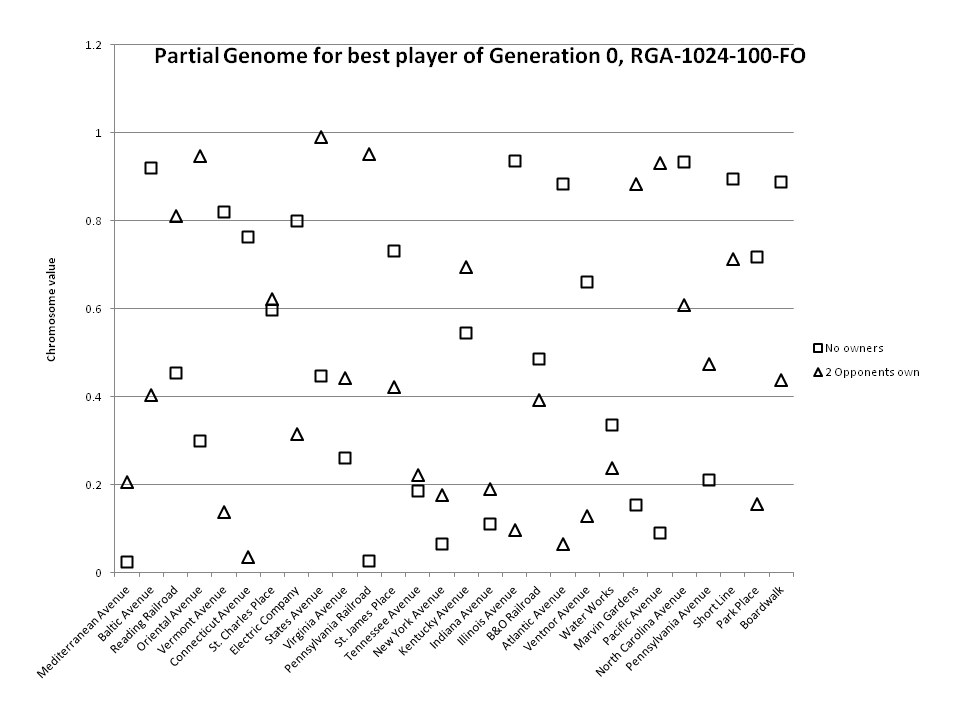
\includegraphics[width=0.75\columnwidth]{Figures/genome000.png}}
\caption[Illustration of Genome, Generation 0]{This chart shows part of the
genome of the fittest player in the first generation of the RGA-1024-100-FO
population. This chart compares the chromosome used when no player owns
any property in the group (represented by the square symbol) against the
chromosome used when two other players own a property in the group (the triangle
symbol).}
\label{figure-genome0}
\end{figure}

\begin{figure}[htp]
\centerline{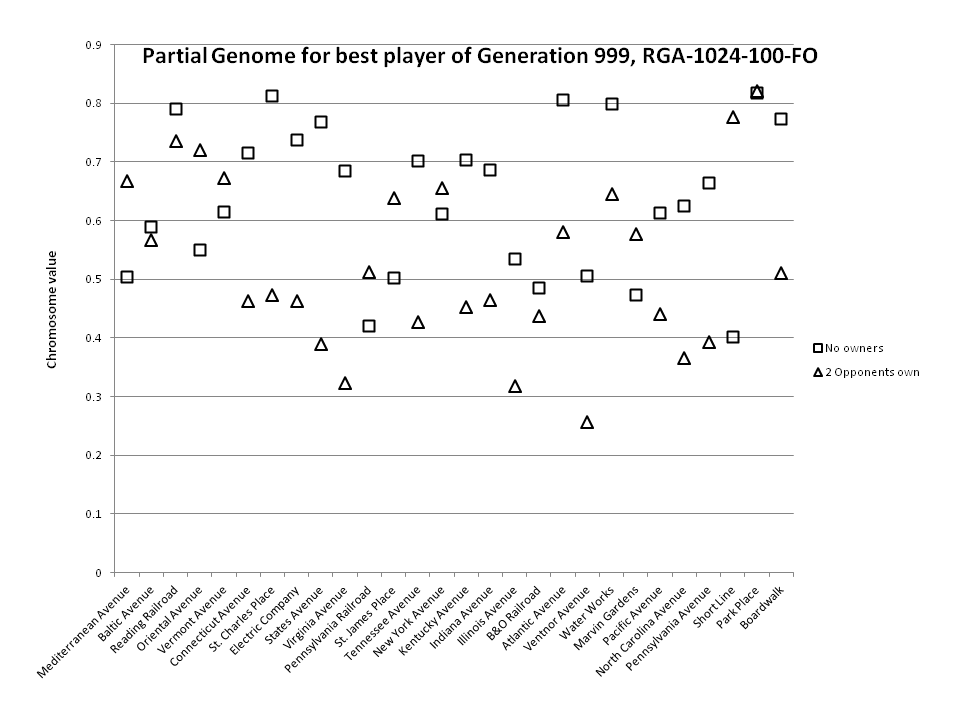
\includegraphics[width=0.75\columnwidth]{Figures/genome999.png}}
\caption[Illustration of Genome, Generation 999]{This chart shows part of the
genome of the fittest player in the last generation of the RGA-1024-100-FO
population. This chart compares the chromosome used when no player owns any
property in the group (the square symbol) against the chromosome used when two
other players own a property in the group (the triangle symbol). These two genes
show agreement with the heuristic strategy: the player is more likely to buy a
property when no one owns a property in the group, and relatively less likely to
buy a property when other players are blocking the group from being
monopolized.}
\label{figure-genome999}
\end{figure}

% Table generated by Excel2LaTeX from sheet 'genome0099 (2)'
\begin{table}[htbp]
  \centering
  \caption[Genome Comparison, Gen 0 vs Gen 999]{Comparison of Best Genomes from Generation 0 and Generation 999}
  \scalebox{0.75}{
    \begin{tabular}{lrrr|rrr}
    \toprule
           & \multicolumn{3}{c|}{Generation 0} & \multicolumn{3}{c}{Generation 999} \\
    \midrule
           & No Owner & 2 Opponents own & Diff   & No Owner & 2 Opponents own & Diff \\
    Mediterranean Avenue & 0.023  & 0.205  & -0.182 & 0.504  & 0.668  & -0.164 \\
    Baltic Avenue & 0.920  & 0.404  & 0.517  & 0.589  & 0.567  & 0.023 \\
    Reading Railroad & 0.454  & 0.810  & -0.356 & 0.790  & 0.736  & 0.054 \\
    Oriental Avenue & 0.300  & 0.947  & -0.648 & 0.550  & 0.721  & -0.171 \\
    Vermont Avenue & 0.821  & 0.138  & 0.683  & 0.614  & 0.673  & -0.059 \\
    Connecticut Avenue & 0.762  & 0.036  & 0.726  & 0.715  & 0.463  & 0.252 \\
    St. Charles Place & 0.598  & 0.622  & -0.024 & 0.812  & 0.473  & 0.339 \\
    Electric Company & 0.799  & 0.314  & 0.484  & 0.737  & 0.463  & 0.274 \\
    States Avenue & 0.448  & 0.991  & -0.543 & 0.768  & 0.389  & 0.379 \\
    Virginia Avenue & 0.260  & 0.442  & -0.182 & 0.685  & 0.323  & 0.362 \\
    Pennsylvania Railroad & 0.027  & 0.952  & -0.925 & 0.421  & 0.512  & -0.091 \\
    St. James Place & 0.730  & 0.423  & 0.308  & 0.502  & 0.639  & -0.137 \\
    Tennessee Avenue & 0.186  & 0.223  & -0.036 & 0.702  & 0.427  & 0.275 \\
    New York Avenue & 0.064  & 0.175  & -0.111 & 0.612  & 0.656  & -0.043 \\
    Kentucky Avenue & 0.544  & 0.694  & -0.150 & 0.704  & 0.452  & 0.252 \\
    Indiana Avenue & 0.110  & 0.189  & -0.080 & 0.686  & 0.465  & 0.221 \\
    Illinois Avenue & 0.936  & 0.096  & 0.840  & 0.536  & 0.319  & 0.217 \\
    B\&O Railroad & 0.487  & 0.391  & 0.095  & 0.485  & 0.437  & 0.048 \\
    Atlantic Avenue & 0.884  & 0.064  & 0.820  & 0.806  & 0.581  & 0.225 \\
    Ventnor Avenue & 0.661  & 0.128  & 0.532  & 0.506  & 0.257  & 0.250 \\
    Water Works & 0.335  & 0.237  & 0.098  & 0.800  & 0.645  & 0.154 \\
    Marvin Gardens & 0.154  & 0.883  & -0.730 & 0.472  & 0.577  & -0.104 \\
    Pacific Avenue & 0.091  & 0.931  & -0.840 & 0.614  & 0.440  & 0.173 \\
    North Carolina Avenue & 0.934  & 0.609  & 0.325  & 0.625  & 0.365  & 0.260 \\
    Pennsylvania Avenue & 0.210  & 0.474  & -0.265 & 0.663  & 0.392  & 0.271 \\
    Short Line & 0.895  & 0.713  & 0.182  & 0.402  & 0.778  & -0.376 \\
    Park Place & 0.718  & 0.155  & 0.563  & 0.818  & 0.822  & -0.004 \\
    Boardwalk & 0.887  & 0.439  & 0.448  & 0.774  & 0.511  & 0.263 \\
    \bottomrule
    \end{tabular}}
  \label{tab:chromo_compare}%
\end{table}%


\clearpage
\chapter{Sample SGA Fitness Distributions}
\label{appendix:SGAFitness}

This appendix contains some sample SGA fitness distributions. As was discussed
in Section~\ref{6_SGA}, the distributions appear to be normal, but quickly show
as skewed character which can be seen in these figures.

\clearpage
\begin{figure}[htp]
\centerline{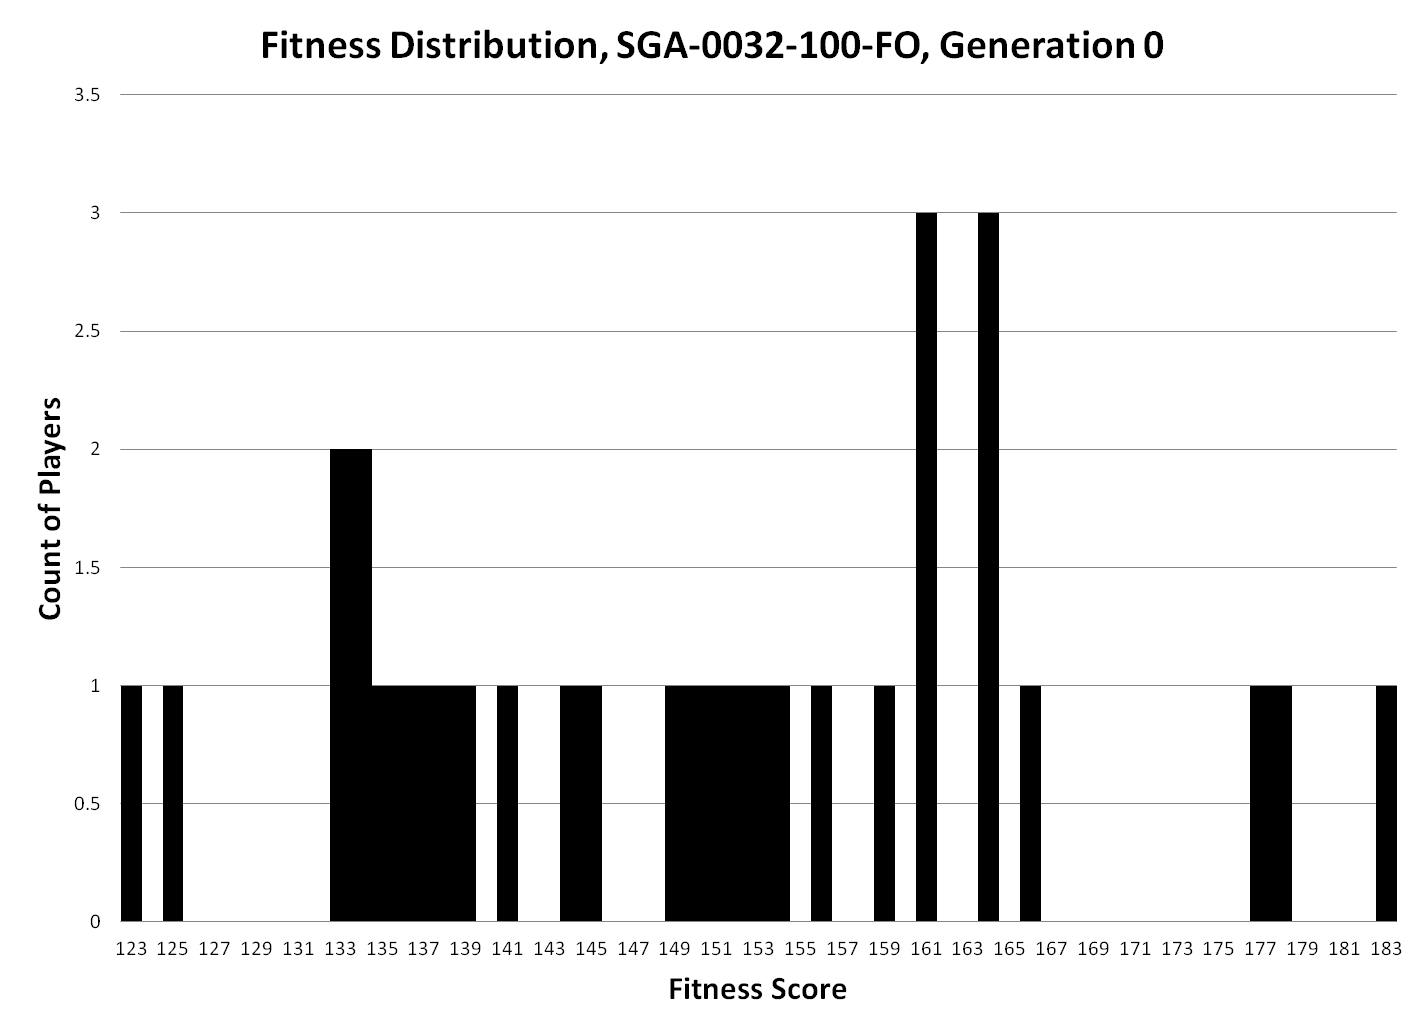
\includegraphics[width=0.75\columnwidth]{Figures/SGA_0032_100_FO_gen000.png}}
\caption{Fitness Distribution, SGA-0032-100-FO, Generation 0}
\end{figure}

\begin{figure}[htp]
\centerline{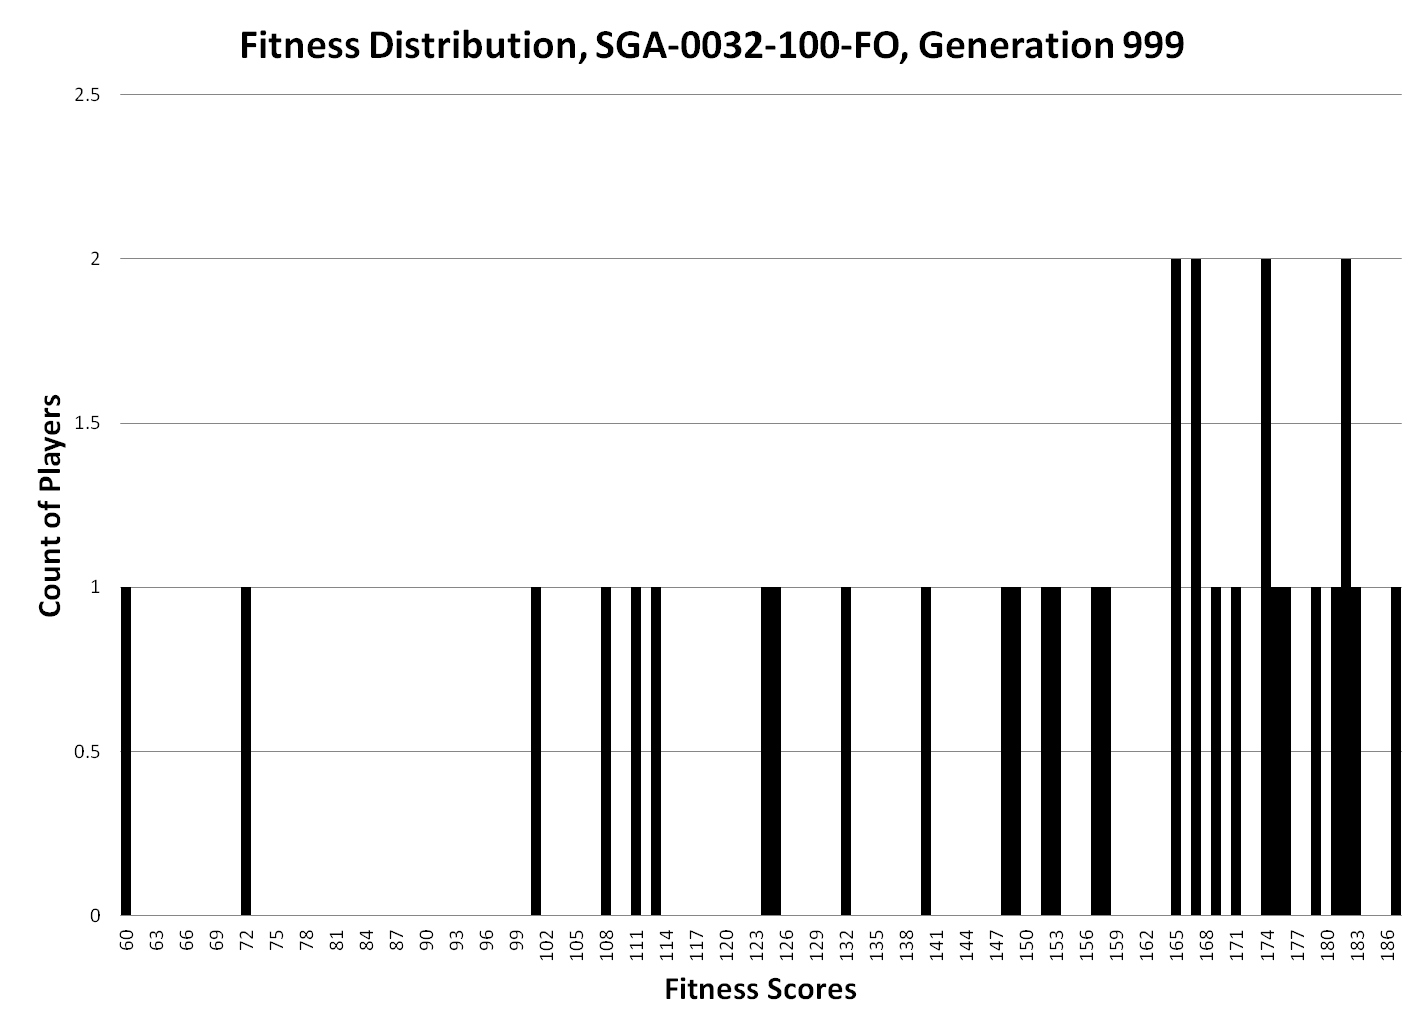
\includegraphics[width=0.75\columnwidth]{Figures/SGA_0032_100_FO_gen999.png}}
\caption{Fitness Distribution, SGA-0032-100-FO, Generation 999}
\end{figure}

\begin{figure}[htp]
\centerline{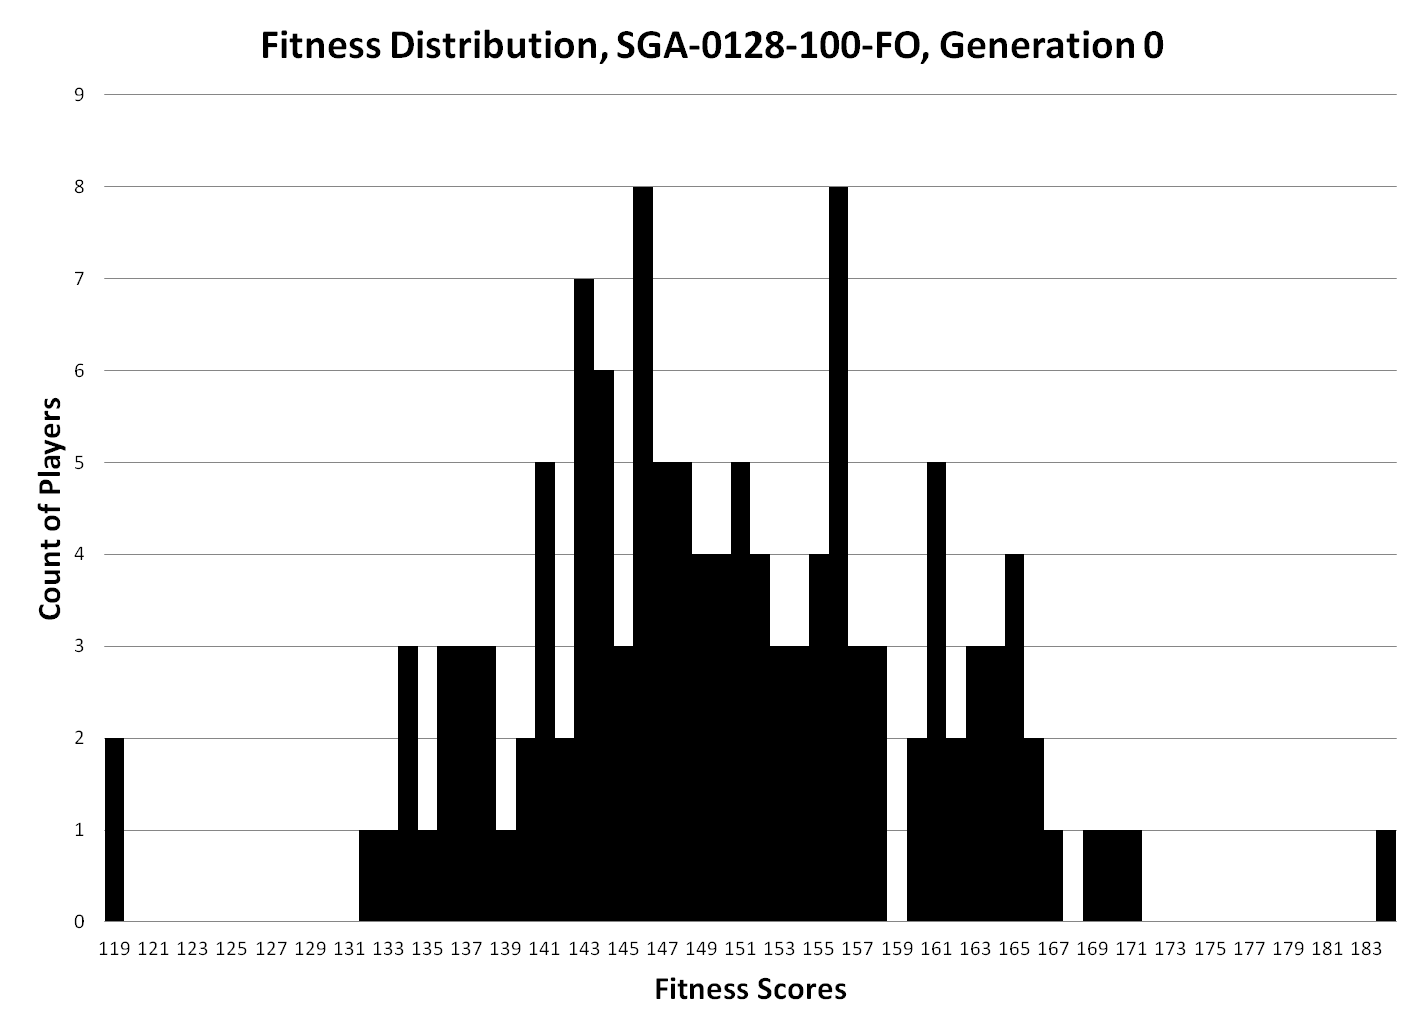
\includegraphics[width=0.75\columnwidth]{Figures/SGA_0128_100_FO_gen000.png}}
\caption{Fitness Distribution, SGA-0128-100-FO, Generation 0}
\end{figure}

\begin{figure}[htp]
\centerline{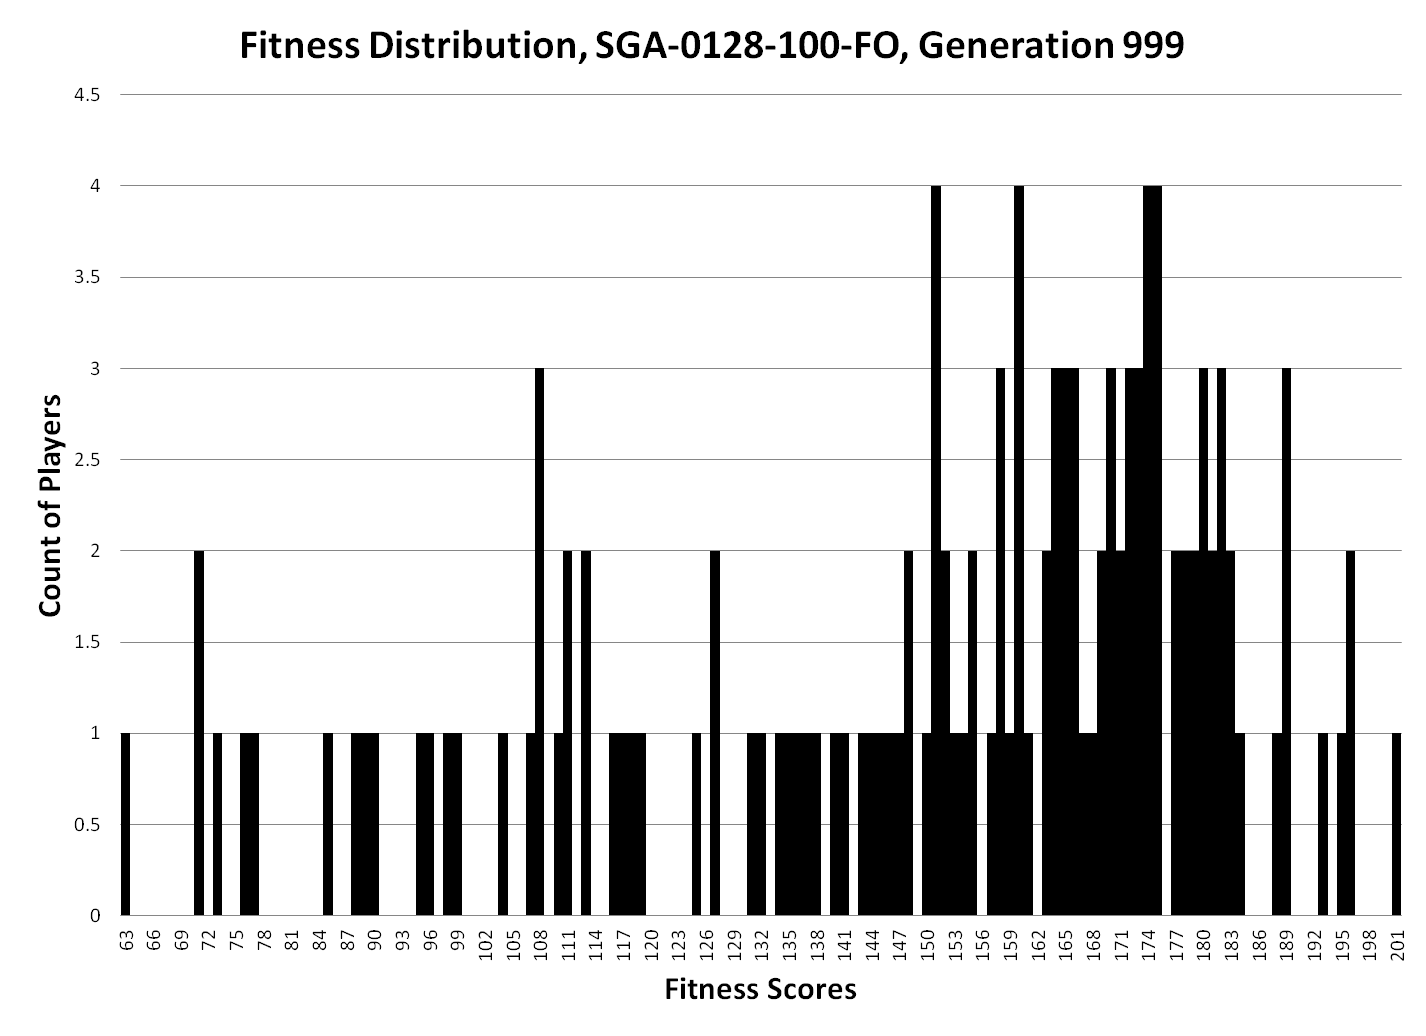
\includegraphics[width=0.75\columnwidth]{Figures/SGA_0128_100_FO_gen999.png}}
\caption{Fitness Distribution, SGA-0128-100-FO, Generation 999}
\end{figure}

\begin{figure}[htp]
\centerline{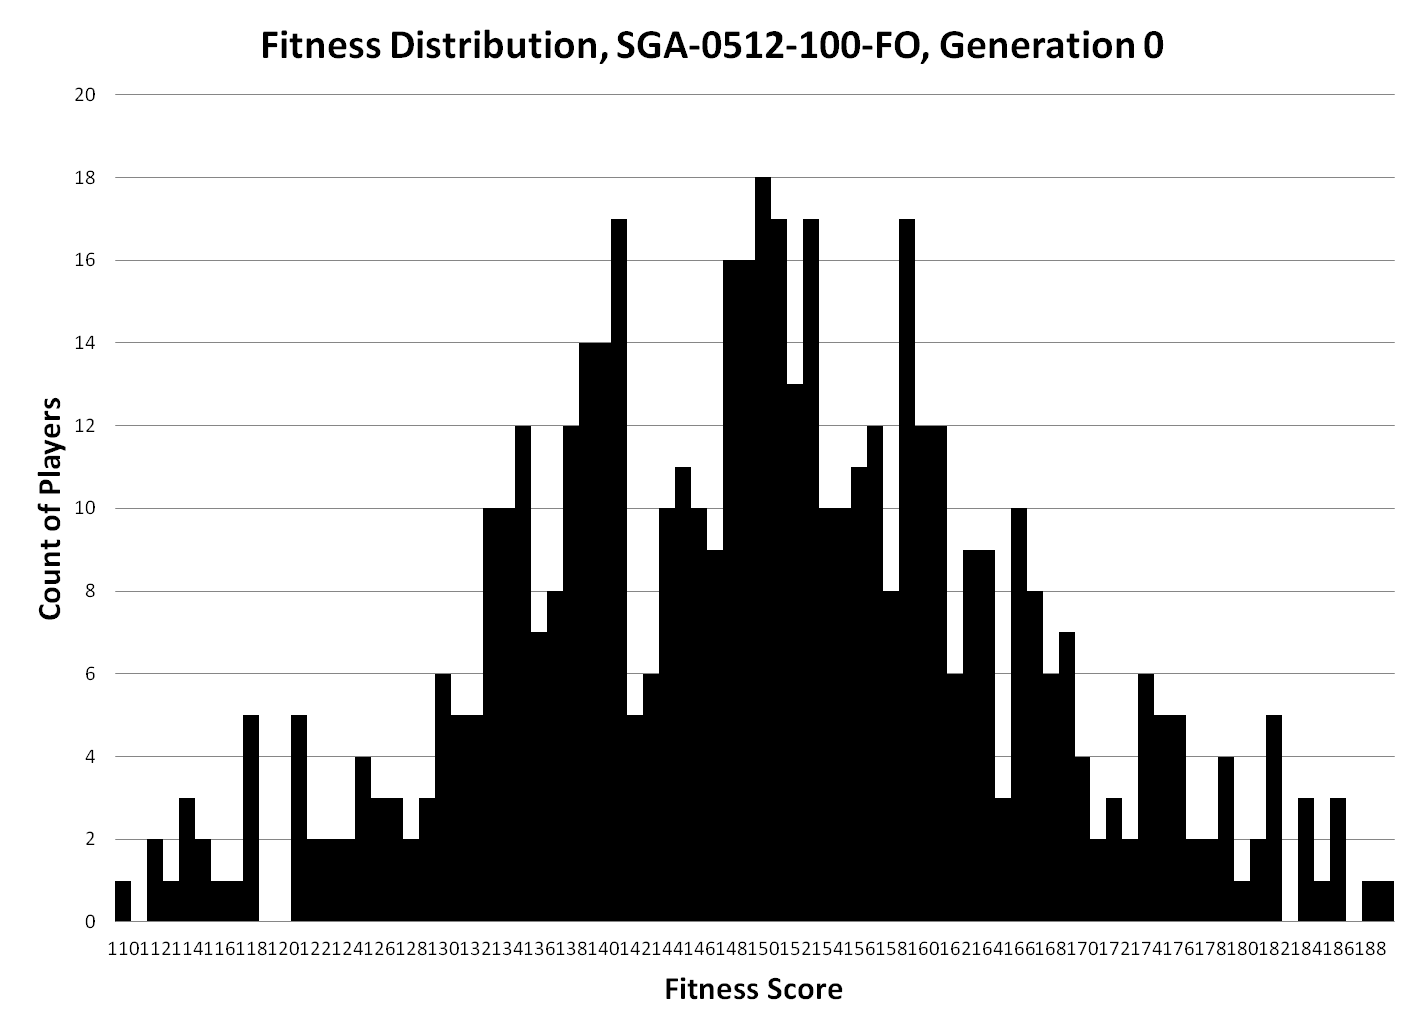
\includegraphics[width=0.75\columnwidth]{Figures/SGA_0512_100_FO_gen000.png}}
\caption{Fitness Distribution, SGA-0512-100-FO, Generation 0}
\end{figure}

\begin{figure}[htp]
\centerline{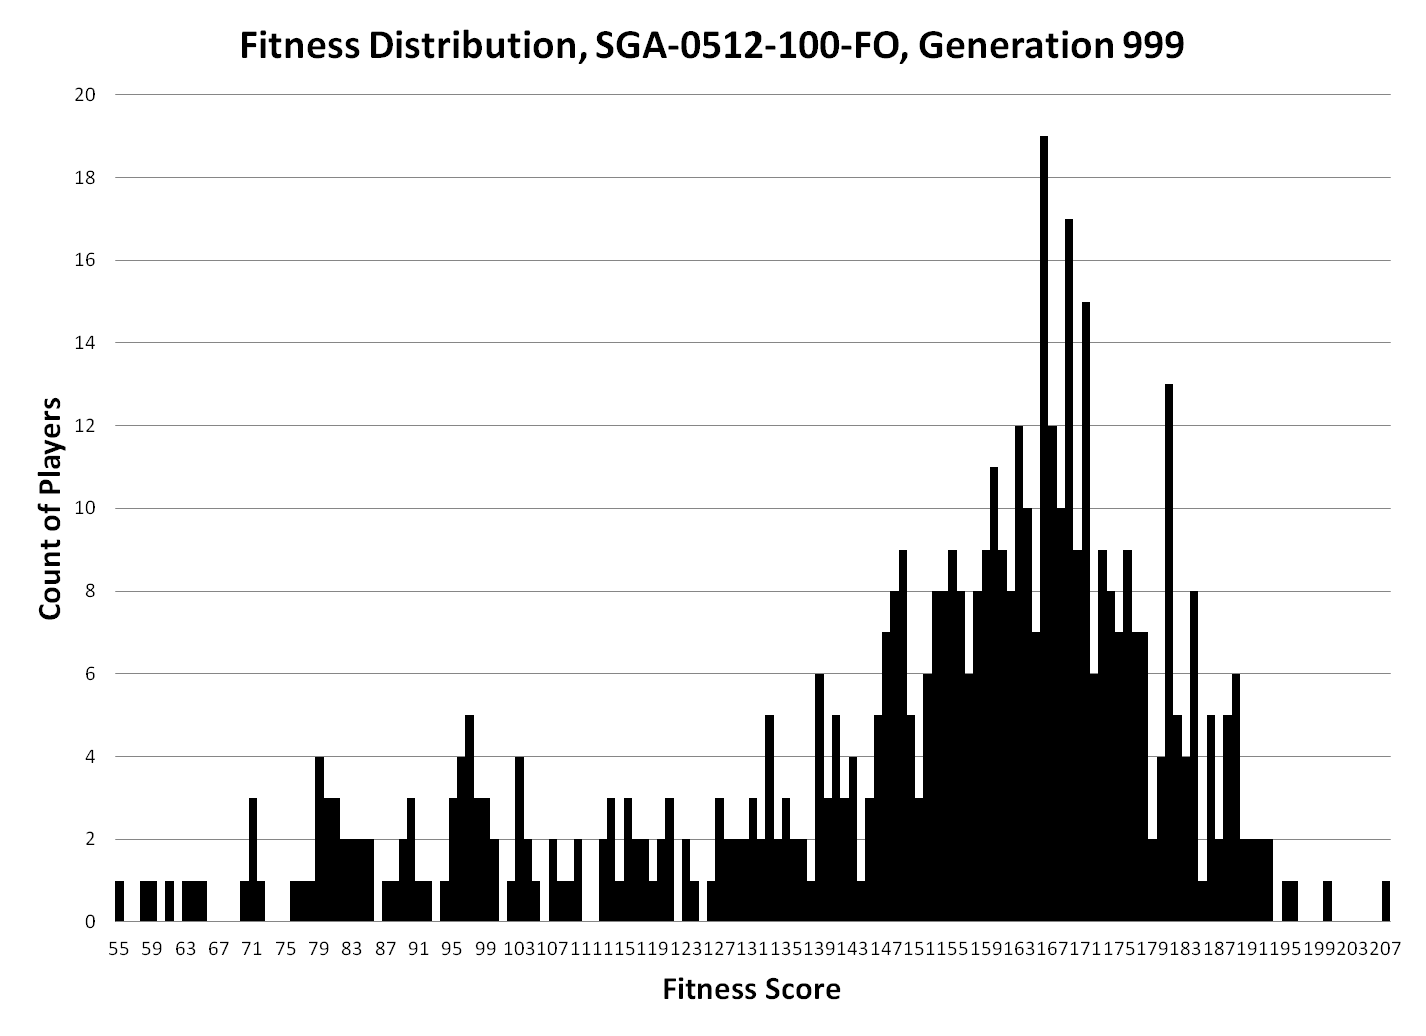
\includegraphics[width=0.75\columnwidth]{Figures/SGA_0512_100_FO_gen999.png}}
\caption{Fitness Distribution, SGA-0512-100-FO, Generation 999}
\end{figure}

\begin{figure}[htp]
\centerline{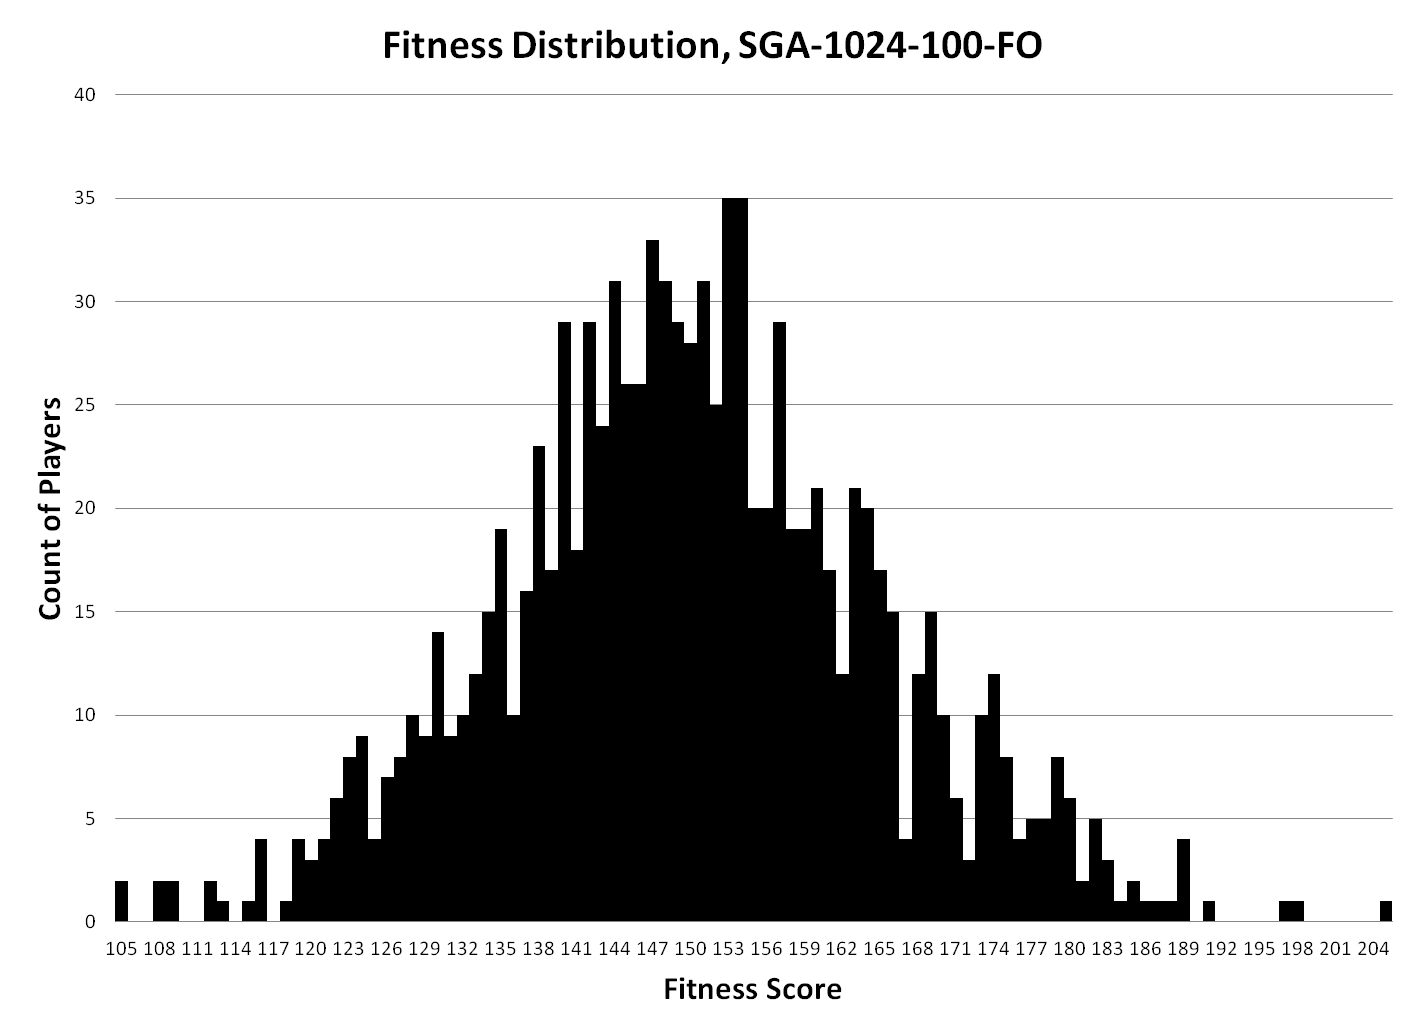
\includegraphics[width=0.75\columnwidth]{Figures/SGA_1024_100_FO_gen0.png}}
\caption{Fitness Distribution, SGA-1024-100-FO, Generation 0}
\end{figure}

\begin{figure}[htp]
\centerline{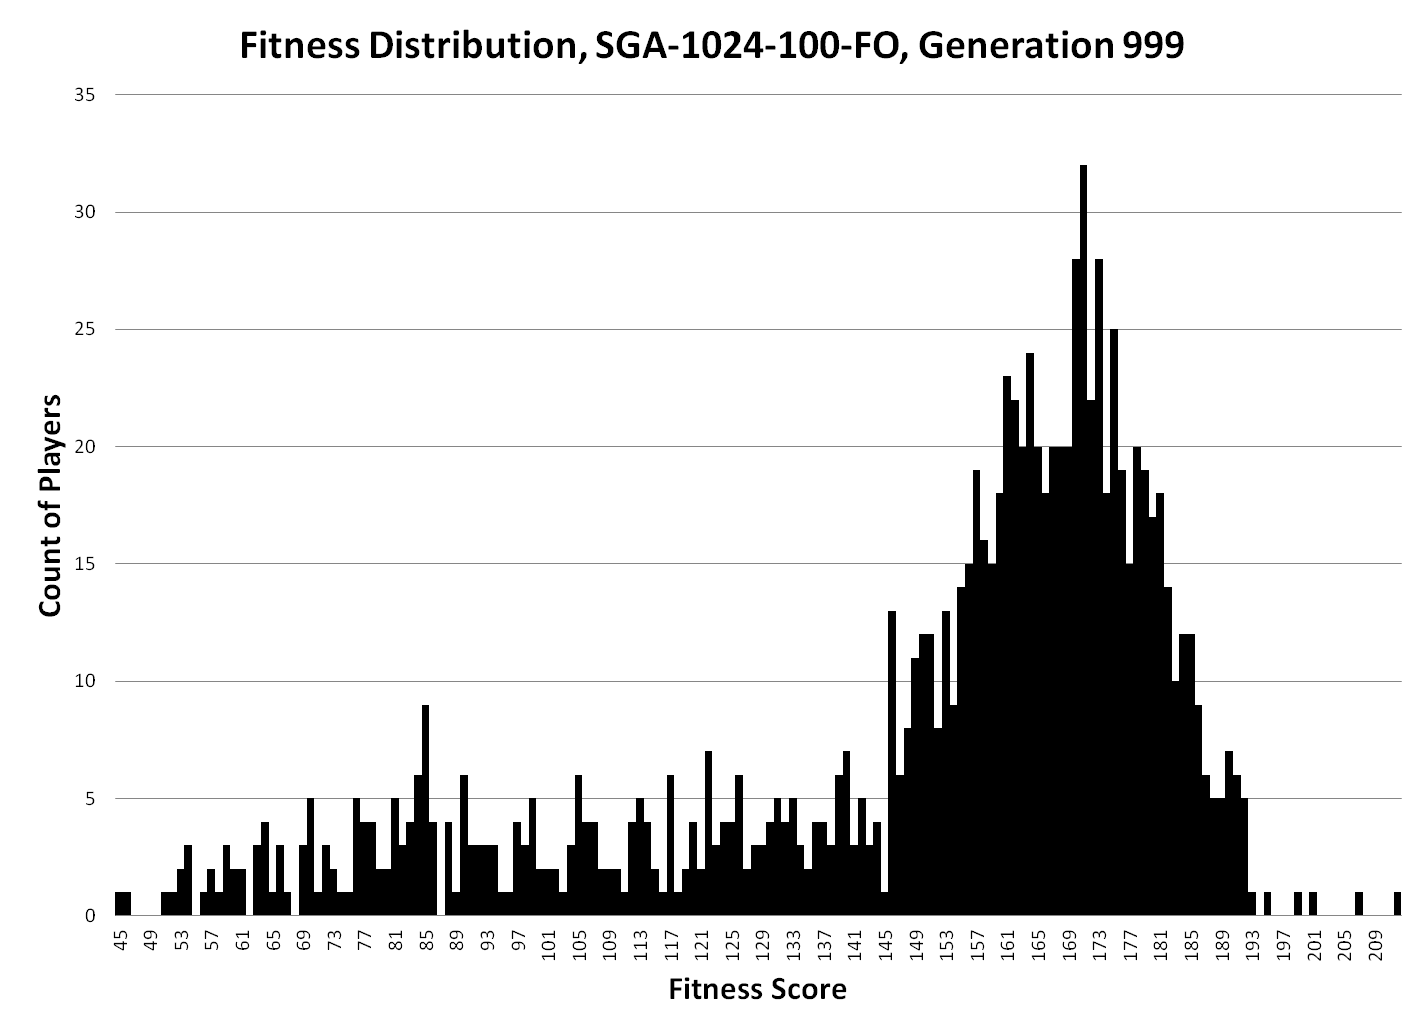
\includegraphics[width=0.75\columnwidth]{Figures/SGA_1024_100_FO_gen999.png}}
\caption{Fitness Distribution, SGA-1024-100-FO, Generation 999}
\end{figure}

\clearpage
%\thispagestyle{empty}
%\addcontentsline{toc}{chapter}{Appendix C: Creative Commons License}
%\setcounter{secnumdepth}{0}
%\setcounter{tocdepth}{1}
%\appendix{{\Large \bf Appendix L: Creative Commons License}}
\newpage
\chapter{Creative Commons License}
\label{sec:appendixLbrief}

This work is licensed under the Creative Commons
Attribution-NonCommercial-NoDerivs 3.0 Unported License. To view a copy of this
license, visit \url{http://creativecommons.org/licenses/by-nc-nd/3.0/} or send a
letter to Creative Commons, 444 Castro Street, Suite 900, Mountain View,
California, 94041, USA.
\section*{Disclaimer} This is a human-readable summary of the Legal Code (the
full license).
\section*{You are free:}
    \textbf{to Share} - to copy, distribute and transmit the work
\section*{Under the following conditions:}
    \textbf{Attribution} - You must attribute the work in the manner specified
    by the author or licensor (but not in any way that suggests that they
    endorse you or your use of the work).

    \textbf{Noncommercial} - You may not use this work for commercial purposes.

    \textbf{No Derivative Works} - You may not alter, transform, or build upon
    this work.
\section*{With the understanding that:}
    \textbf{Waiver} - Any of the above conditions can be waived if you get
    permission from the copyright holder.

    \textbf{Public Domain} - Where the work or any of its elements is in the
    public domain under applicable law, that status is in no way affected by the
    license.

    \textbf{Other Rights} - In no way are any of the following rights affected
    by the license:
      \begin{itemize} 
        \item {Your fair dealing or fair use rights, or other applicable
      copyright exceptions and limitations;} 
        \item {The author's moral rights;} 
        \item {Rights other persons may have either in the work itself or in how
      the work is used, such as publicity or privacy rights.}
      \end{itemize}
\section*{Notice}
For any reuse or distribution, you must make clear to others the license terms
of this work. 

\end{document}
